\documentclass[a4paper,12pt]{report}



\usepackage[spanish]{babel} \usepackage[T1]{fontenc}
\usepackage{times} \usepackage[utf8]{inputenc}
%\usepackage{parskip}
\usepackage{amsmath}
\usepackage{verbatim} 
\usepackage{spverbatim}
\usepackage[usenames,dvipsnames]{color}
\usepackage{colortbl}
\usepackage{color}
\usepackage{listings}

\lstset{ %
  backgroundcolor=\color[gray]{.95},   % choose the background color; you must add \usepackage{color} or \usepackage{xcolor}
  basicstyle=\footnotesize,
  literate=
  {á}{{\'a}}1 {é}{{\'e}}1 {í}{{\'i}}1 {ó}{{\'o}}1 {ú}{{\'u}}1
  {Á}{{\'A}}1 {É}{{\'E}}1 {Í}{{\'I}}1 {Ó}{{\'O}}1 {Ú}{{\'U}}1
  {à}{{\`a}}1 {è}{{\'e}}1 {ì}{{\`i}}1 {ò}{{\`o}}1 {ò}{{\`u}}1
  {À}{{\`A}}1 {È}{{\'E}}1 {Ì}{{\`I}}1 {Ò}{{\`O}}1 {Ò}{{\`U}}1
  {ä}{{\"a}}1 {ë}{{\"e}}1 {ï}{{\"i}}1 {ö}{{\"o}}1 {ü}{{\"u}}1
  {Ä}{{\"A}}1 {Ë}{{\"E}}1 {Ï}{{\"I}}1 {Ö}{{\"O}}1 {Ü}{{\"U}}1
  {â}{{\^a}}1 {ê}{{\^e}}1 {î}{{\^i}}1 {ô}{{\^o}}1 {û}{{\^u}}1
  {Â}{{\^A}}1 {Ê}{{\^E}}1 {Î}{{\^I}}1 {Ô}{{\^O}}1 {Û}{{\^U}}1
  {œ}{{\oe}}1 {Œ}{{\OE}}1 {æ}{{\ae}}1 {Æ}{{\AE}}1 {ß}{{\ss}}1
  {ç}{{\c c}}1 {Ç}{{\c C}}1 {ø}{{\o}}1 {å}{{\r a}}1 {Å}{{\r A}}1
  {€}{{\EUR}}1 {£}{{\pounds}}1
}
  
\setcounter{secnumdepth}{6}
\setcounter{tocdepth}{6}
\definecolor{orange}{RGB}{0,0,255}
\usepackage{graphicx} 
\usepackage{subfigure}
\usepackage[utf8]{inputenc}
%\usepackage[Conny]{fncychap}
%\usepackage[Rejne]{fncychap}
%\usepackage[Bjarne]{fncychap}
%\ChTitleVar{\vspace{1.5cm}\centering\Huge\rm\bfseries}
%\ChNameVar{\vspace{1.5cm}\centering\Huge\rm\bfseries}

\hyphenation{sis-te-má-ti-co pa-leo-lí-ti-co con-ti-nua-men-te pe-ri-fé-ri-co de-sa-rro-lla-do-res pro-ble-mas fa-bri-can-te}

\usepackage{titlesec}

\titleclass{\part}{top} % make part like a chapter
\titleformat{\part}
[display]
{\centering\normalfont\Huge\bfseries}
{\titlerule[5pt]\vspace{3pt}\titlerule[2pt]\vspace{3pt}\MakeUppercase{\partname} \thepart}
{0pt}
{\titlerule[2pt]\vspace{1pc}\huge\MakeUppercase}
\titlespacing*{\part}{0pt}{0pt}{20pt}

\titleclass{\chapter}{straight} % make chapter like a section (no newpage)
\titleformat{\chapter}
[display]
{\centering\normalfont\Huge\bfseries}
{\titlerule[5pt]\vspace{3pt}\titlerule[2pt]\vspace{3pt}\MakeUppercase{\chaptertitlename} \thechapter}
{0pt}
{\titlerule[2pt]\vspace{6pt}\huge\MakeUppercase}
\titlespacing*{\chapter}{0pt}{0pt}{40pt}

%\usepackage{makeidx}
\definecolor{DarkBlue}{rgb}{0.1,0.1,.1}
\usepackage[linkcolor=DarkBlue,urlcolor=DarkBlue,colorlinks,breaklinks]{hyperref}
\usepackage[left=2.5cm,top=3.0cm,right=2.5cm,bottom=3.0cm]{geometry} 
\usepackage{fancyhdr}
\pagestyle{fancy}
\fancyhf{}
\fancyhead[L]{\leftmark} %\fancyhead[R]{\rightmark}
\fancyfoot[L]{Gomez, Roberto Pablo - Lovaisa Michelini, Valeria}
\fancyfoot[R]{P\'agina: \thepage} %\fancyfoot[LE,RO]{P\'agina: \thepage}                               
\renewcommand{\headrulewidth}{1.0pt}
\renewcommand{\footrulewidth}{0.4pt}

\begin{document}
\setlength{\parindent}{12pt}
\setlength{\parskip}{3mm}

\title{\vspace{-4cm} \textbf{Proyecto Integrador \\ \line(1,0){350}}\\
  \vspace{0.5cm}\centering{
\includegraphics[scale=0.53]{images/logoUNC.png}}\\}
\author{\vspace{-0.25cm} Autor \vspace{0.25cm}\\ Gomez, Roberto Pablo - Lovaisa
Michelini Valeria \bigskip \bigskip \bigskip \\
  Tema \vspace{0.25cm} \\ \textbf{Implementación de un Sistema en Chip con Microprocesador  }\\ \textbf{ Soft-Core y soporte Linux} \\ \textbf{}
  \bigskip \bigskip \bigskip \bigskip\\
  \begin{normalsize}Director PI\end{normalsize}\\
  \begin{normalsize}Ing. Mgter. Micolini, Orlando \end{normalsize} \\
  \begin{normalsize}Director del Laboratorio de Arquitectura de Computadoras FCEFyN-UNC\bigskip \bigskip \end{normalsize} \\
  \begin{normalsize}CoDirector PI\end{normalsize} \\
  \begin{normalsize}Ing. Paredes, Federico  \end{normalsize}\\ 
  \begin{normalsize}Integrante del Centro Universitario De Automatización y Robótica-UTN-FRC\bigskip \bigskip \end{normalsize}\\
  }
\date{}

\maketitle{}

\newpage
\tableofcontents{}

\newpage
\listoffigures{}

\newpage
\listoftables{}

%%%%%%%%%%%%%%%%%%%%%%%%%%%%%%%%%%%%%%%%%%%%%%%%%%%%%%%%%%%%%%%%%%%%%%%%%%%%%%%%%%%%%%%%%%%%%%%%%%%%%%%%%%%%%%%%%%%%%

\newpage
%\chapter{Introducción}

\section{Descripción General}
Se implementará un sistema en chip (SoC) con microprocesador Soft-Core sobre FPGA. El proyecto estará bajo el paradigma de software libre incluyendo
el código RTL del SoC, las herramientas de desarrollo y los Sistema Operativos. Inicialmente se analizarán las diferentes alternativas de
Microprocesadores Soft-Core que permitan su implentación en proyectos SoC Open-Source tales como MinSoC y ORPSoC. El elemento central de
ambos proyectos es el microprocesador soft OpenRisc1200, de capacidades comparables a los microprocesadores soft MicroBlaze de Xilinx y NiOS II de
Altera. Este procesador está soportado por el compilador GCC y permite correr el sistema operativo Linux. El funcionamiento del sistema se comproborá
implementándose sobre un Kit XtremeDSP Starter Platform disponible en el Centro Universitario de Automatización y Robótica UTN-FRC.

\section{Objetivos}
\subsection{Objetivo General}

Implementar un System on Chip OpenSource con Microprocesador Softcore embebido que soporte un Sistema Operativo libre, con la finalidad de entregar
un sistema integral FPGA-SoC-Sistema Operativo completamente funcional y bajo licencia GPL v2. %o LGPL

\subsection{Objetivo Específico}
\begin{itemize}
\item Seleccionar, analizar y determinar la factibilidad de implementación de un microprocesador Softcore en FPGA.
% No es seleccionar el SoC tamb 
\item Establecer un System on Chip Open Source donde poder implementar un Softcore.
%o LGPL ???
\item Determinar los Sistemas Operativos con licencia GPL v2 que poseean las prestaciones funcionales adecuadas para su utilización en Sistemas
Embebidos de propósito específico(Por ej.: Sistemas de tiempo real).
\end{itemize}

\section{Motivación} 

Existe un grupo de cores Softcore de código abierto que no están limitados por la tecnología. Los cores destacados de microprocesadores de 32 bits,
son los procesadores SPARC LEON OpenRISC 1200 , y el core de LatticeMico32. Usar cores de código abierto va unido a una serie de conceptos como:
\begin {itemize}
\item
\textit{Flexibilidad}  Si el código fuente está disponible, los desarrolladores pueden modificar el código de acuerdo a sus necesidades. Además, se
produce un flujo constante de ideas que mejoran la calidad del código.
\item 
\textit{Fiabilidad y seguridad}  Con muchos programadores a la vez escrutando el mismo trabajo, los errores se detectan y corrigen antes, por lo que
el producto resultante es mas fiable y eficaz que el comercial.
\item 
\textit{Rapidez de desarrollo}  Las actualizaciones y ajustes se realizan a través de una comunicación constante vía Internet.
\item 
\textit{Relación con el usuario} El programador se acerca mucho mas a las necesidades reales de su cliente, y puede crear un producto específico para
él.
 \end {itemize}
 
Obtener un Sistema Integral de código abierto en donde se tiene código HDL, assembler y C disponible para adaptarse de acuerdo a los requerimientos
del proyecto, además de la capacidad de migrar de una plataforma a otra logrando menor dependencia entre el código fuente y la plataforma
objetivo. La portabilidad del código abierto nos permite implementarlo sobre un ASICs (Application-specific integrated circuit) o con modificaciones
menores en cualquier FPGA (Field Programmable Gate Array) de Xilinx, Altera, Lattice, etc. Estos tres de los más grandes proveedores de FPGA  %,% Xilinx , Altera y Lattice ,
ofrecen sus propios microcore RISC de 32bits como lo son Nios de  Altera y Microblaze de Xilinx  Son micro cores en donde el código fuente RTL no se
encuera disponible y solo pueden ser implementados en las FPGA del propio fabricante.

Una de principales ventajas de usar plataformas con FPGA, es que son flexibles y pueden adaptarse a diferentes funciones. Los componentes de
hardware ofrecen mucho mayor rendimiento que el software equivalente. Los cuellos de botella de procesamiento del sistema pueden identificarse y
sustituirse por hardware, de manera que se evita la costosa optimización del software.

\section{Importancia del Problema}

En el diseño del sistema embebido se usan diferentes procesos dependiendo del tipo de sistema, el hardware disponible y la organización que
desarrolle el sistema. Una de las actividades principales en un proceso de diseño de software es la elección del hardware y del sistema operativo que
se efectúa antes del desarrollo del software. Ante tal situación, se debe diseñar el software considerando las restricciones impuestas por las
capacidades del hardware.
Los efectos que influyen dichas elecciones comprenden restricciones de temporización sobre el sistema, limitación en la energía disponible,
experiencia del equipo de desarrollo y límites en el costos del sistema entregable.
 
Se está explorando una línea donde se busca dar al diseñador del sistema embebido una solución flexible en la primera etapa de la elección de
plataforma. Donde a través del análisis de diferentes plataformas de desarrollo OpenSource y privativas se pueda elegir la mejor opción para el tipo
de sistema a desarrollar y los requerimientos de procesamiento.
 
Una vez que se ha elegido la plataforma de ejecución para el sistema, se ha diseñado una arquitectura de proceso y se ha determinado una política de
planeación, es necesario comprobar que el sistema cumplirá sus con sus requerimientos.

\section{Modelo de Desarrollo}

El modelo de desarrollo a utilizar es el Modelo en Espiral tipificado por Ian Sommerville\cite{Etiqueta00}% . El modelo en espiral de ingeniería de software,mostrado en la figura 1.1
, fue originalmente propuesto por Boehm en año 1988, en su artículo "A Spiral Model of Software Development and Enhancement". Propuso un
marco del proceso de software dirigido por el riesgo. Aquí, el proceso de software se representa como una es espiral, cada ciclo en la espiral
representa una fase del proceso de software. Por ende, el ciclo más interno puede relacionarse con la factibilidad del sistema, el siguiente ciclo
con la definición de requerimientos, el siguiente ciclo al diseño del sistema, y así sucesivamente. %Aclarar que lo implementamos para implementar
% HW...

\begin{figure}[h!]
 \begin{center}
  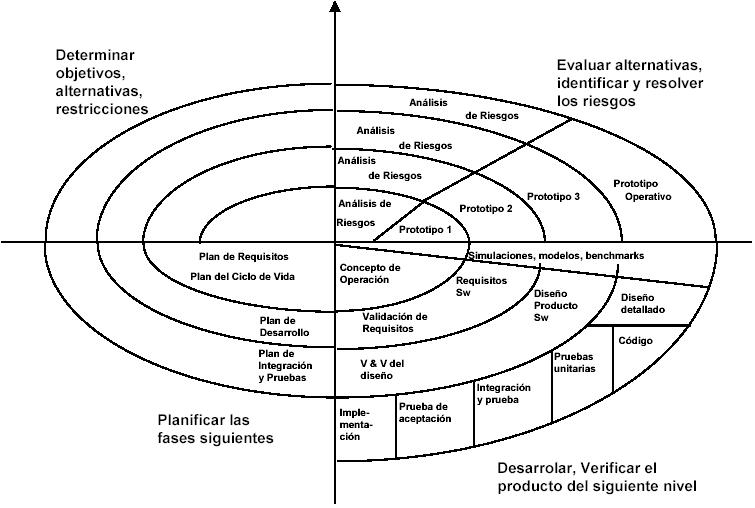
\includegraphics[width=0.5\textwidth,keepaspectratio=true]{./images/ESPIRAL}
  \caption{Etapas del modelo de desarrollo en espiral}
  \label{fig:esquema}
 \end{center}
\end{figure}

Cada ciclo del espiral se divide en 4 sectores:
 
\begin {itemize}
\item 
\textit{Establecimiento de objetivo}  Se definen objetivos específicos para dicha fase del proyecto. Se identifican restricciones en el proceso y el
producto y se traza un plan detallado de gestión. Se identifican los riesgos del proyecto. Dependiendo de estos riegos, se planean estrategias
alternativas que permitan utilizar otros caminos hacia la solución ante sobre la aparición de problemas asociados a estos riesgos.
\item 
\textit{Validación y reducción del riesgo}  En cada uno de los riesgos identificados del proyecto, se realiza un análisis minucioso proponiendo
acciones para reducir dichos riesgos.
\item 
\textit{Desarrollo y validación}  Después de una evaluacion de riesgos, se elige un modelo de desarrollo para el sistema.
\item 
\textit{Planeamiento}  El proyecto se revisa y se toma una decisión sobre si hay que continuar con otro ciclo de la espiral. Si se opta por continuar,
se trazan los planes para la siguente fase del proyecto.
\end {itemize}

Como característica principal de esta metodología es que posee una consideración explícita del riesgo. Informalmente, el riesgo significa
sencillamente que algo puede ir mal. Los riegos originan problemas en el proyecto, como los de confección de agendas y excesos en los costos, por lo
tanto, la disminución de riegos es una actividad sumamente importante en la gestión del proyecto. Un ciclo en la espiral comienza con la elaboración
de objetivos, como el rendimiento y la funcionalidad. Entonces se enumeran formas alternativas de alcanzar estos objetivos y las restricciones
impuestas en cada una de ellas. Cada alternativa se evalúa contra cada objetivo y se identifican las fuentes de riegos del proyecto. El siguiente
paso es resolver estos riesgos mediante actividades de recopilación de información como la de detallar más el análisis, la construcción de prototipos
y la simulación. Una vez que se han evaluado los riesgos se llevará a cabo cierto desarrollo, seguido de una actividad de planificación para la
siguiente fase del proceso.

%El softcore OpenRisc  que se encuentra en el SoC OrpSoc y MinSoc se tiene que implementado en una FPGA  Spartan 3A de Xilinx. Tenemos como fin montar un Linux para validar y verificar el sistema global entregando un sistema funcional bajo licencia libre.
%Actualmente las FPGAs nos birndan la posibilidad de implementar estos proyectos, donde el Hardware y el Software son una misma entidad. Este nuevo enfoque nos permite aprovechar la facilidad de implementar soluciones por Hardware.

\section{Alcance de Estudio}
%En cada etapa ????
Debido al plazo estipulado para el desarrollo del proyecto, el mismo involucra tres etapas: 

\begin {itemize}
\item Especificación y Análisis de requerimientos.
\item Implementación.
\item Testing.
\end {itemize}


\section{Metodología}
%% Primera vez en la facultad???
Considerando que el objetivo planteado es un desarrollo que se realiza por primera vez, se aplicará un desarrollo experimental y de simulación. La
falta de documentación al respecto y al ser un desarrollo de vanguardia son factores que acentúan en esta decisión. Sumado a lo dicho anteriormente,
en el laboratorio donde se desarrolla este proyecto no existen antecedentes de trabajos similares que involucren Microprocesadores Softcore.


%% Esto esta incompleto. 
Se utilizó como metodología en esta implementación el modelo de componentes que define estándares para tal fin, documentación y el
despliegue de componentes.





%%%%% poner en negrita asi \textit{Python} 


 % Intro
\begin{part}{Marco Teórico}
\newpage
%\chapter{FPGA, Microprocesadores Soft-Core y IP-Core}
\section{FPGAs}
	\subsection{Introducción}
	La fabricación de dispositivos semiconductores es un proceso complicado de plazos largos y costosos. Esto lleva a que los diseños destinados para la 
	implementación en chip de silicio tengan poca oportunidad de ser prototipados antes de que comience la producción en grandes volúmenes. Esto supone
	una gran importancia en las fases de prueba y verificación de un diseño antes de ser fabricado.
	
	Basándose en la predicción de la ley de Moore donde expresa que aproximadamente cada dos años se duplica el número de transistores en un circuito
	integrado\cite{Etiqueta02}, Ross Freeman postuló que los transistores serian menos costoso cada año, haciendo asequible la fabricación de chips
	programables personalizables \cite{Etiqueta03}. La compañía Xilinx, ofreció su primer chip en 1984, que contiene arreglo  celdas lógicas (LCAs),
	programables por el usuario en casi cualquier configuración que requieran. Estos se conocen como (\textit{FPGAs}) .
	
	Las \textit{FPGAs} desempeñan un papel dual, uno como objetivo final de ejecución en un diseño y otro papel como prototipo para la implementación
	definitiva de un diseño. Su capacidad de reconfigurar el diseño parcial o totalmente para su actualización o corrección de errores tiene un costo
	relativamente bajo a diferencia del prototipado sobre ASICs. Actualmente las \textit{FPGA} cuentan con una gran cantidad de recursos disponibles
	(Compuertas lógicas , Bloques de RAM) para implementar diseños digitales complejos. Una desventaja de las \textit{FPGA} es debido a la naturaleza
	inherente de su arquitecturas, los diseños implementados en \textit{FPGA}, comparados con los implementados en ASIC, en general tienen mas area,
	menos porformance y consumen mas energía.
	
	A medida que fue pasando el tiempo las FPGAs fueron disminuyendo su costo y mejoraron la eficiencia en el consumo de energía llevándolas a ser
	consideradas como solución a la implementación de ciertas aplicaciones en lugar de un ASIC. Si los criterios tales como el tiempo de
	comercialización y capacidad de actualización son críticos, con el máximo rendimiento y un consumo reducido de energía, una implementación en FPGA
	puede ser adecuada.
	
	Las FPGAs del presente siglo poco tienen que ver con las primeras aparecidas en los 80, y ofrecen densidades de millones de puertas lógicas además
	de microprocesadores empotrados, interfaces de entrada/salida de alta velocidad, bancos de memoria, multiplicadores hardware, DSPs, etc. El
	resultado final es que las FPGAs de hoy en día permiten implementar una gran variedad de sistemas electrónicos: dispositivos de comunicaciones,
	complejos algoritmos de procesamiento de señal, microprocesadores, etc.

	\subsection{Arquitectura}
    Las \textit{FPGAs} son circuitos integrados digitales que contienen bloques de lógica configurable (CLBs) e interconexiones también configurables entre dichos
	bloques, que permiten al desarrollador programarlas para realizar diversas tareas. Xilinx tiene una estructura básica de matriz simétrica (Figura
	~\ref{fig:compfpga}) que ha sido mantenida en sus modernas familias de FPGA, aumentando con cada nueva familia la capacidad de las CLBs e
	interconexiones.
	
	Los componentes de una \textit{FPGA} de Xilinx (Figura ~\ref{fig:compfpga}) son:

	\begin {itemize}
	\item  Bloques lógicos configurables y Lookup Tables.
	\item  Bloques de entrada y salida.
	\item  Bloques multiplicadores.
	\item  Bloques Manejadores de Clock Digitales.
	\end {itemize}

	\begin{figure}[h!]
 	\begin{center}
   	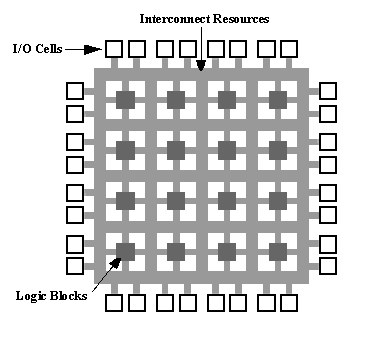
\includegraphics[width=0.5\textwidth,keepaspectratio=true]{./images/fpga1a}
  	\caption{Componentes de una FPGA}
  	\label{fig:compfpga}
 	\end{center}
	\end{figure}

	Otros fabricantes han optado por otro tipo de estructuras internas para sus \textit{FPGAs}, cada una con sus propias ventajas e inconvenientes. No es objeto
	de este trabajo evaluar las estructuras internas de las \textit{FPGAs}.
	
		\subsubsection{Bloques lógicos configurables y lookup tables}
		Todas las\textit{FPGAs} se basan en arrays de pequeños elementos de lógica digital. Los problemas de lógica digital se descomponen en circuitos
		lógicos que puedan ser mapeados a una o más de estas “celdas lógicas” a través de un proceso llamado \textit{“technology mapping"}.
	
		Cada bloque de lógica configurable varía de acuerdo a su fabricante, en el caso de Xilinx tienen el nombre \textit{Logic cell} (LC) (Figura
		~\ref{fig:complc}) contiene una LUT de cuatro entradas, un multiplexor y un registro. Se puede configurar la polaridad del clock, el clock enable y
		la señal de reset.

		\begin{figure}[h!]
		\begin{center}
 		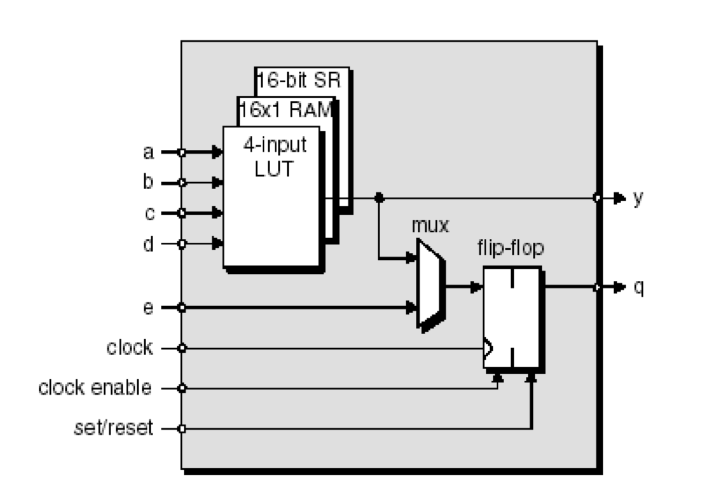
\includegraphics[width=0.5\textwidth,keepaspectratio=true]{./images/celda}
  		\caption{Componentes de una celda lógica}
  		\label{fig:complc}
 		\end{center}
		\end{figure}

		También se encuentran las \textit{Lookup Tables}, que son elementos lógicos que están compuestos de al menos un registro programable (flip\-flop) y
		alguna lógica de entrada, que usualmente está implementada como una \textit{lookup table} de n entradas, donde n es 5 o menos. Estas \textit{LUTs}
		son capaces de implementar cualquier función combinacional de sus entradas.

		\subsubsection{Bloques de entrada y salida de propósito general}
		Las \textit{FPGAs} poseen pines TTL, CMOS, PCI, LVDS y muchos otros que les permiten hacer de interface y convertir tecnologías diferentes.
		Las \textit{FPGAs} tienen bloques de I/O dedicados para clocks y resets globales.
	
		También incluyen PLL y esquemas para el manejo de clocks permitiendo múltiples dominios de los mismos. Las \textit{FPGAs} actuales tienen
		impedancias de I/O configurables, permiten el uso de resistencias internas terminales cuyos valores pueden ser configurados por el usuario.

		\subsubsection{Multiplicadores}
		Algunas funciones como los multiplicadores son muy lentos si se implementan mediante la conexión de un gran numero de bloques lógicos. Por eso
		muchas \textit{FPGAs} incorporan bloques \textit{multiplicadores} hardware (Figura ~\ref{fig:mult}). Estos bloques se encuentran muy cerca de los
		bloques de RAM embebidos.
		
		\begin{figure}[h!]
 		\begin{center}
 		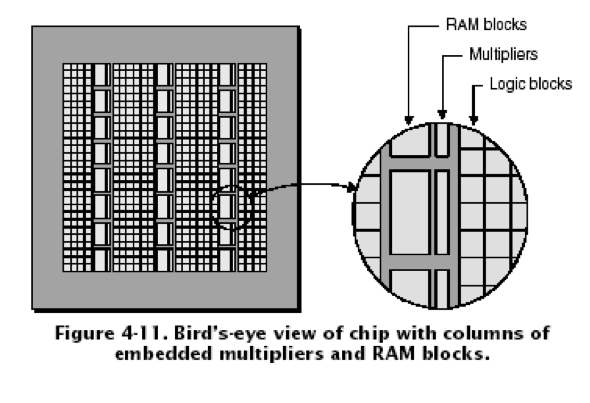
\includegraphics[width=0.5\textwidth,keepaspectratio=true]{./images/multram}
  		\caption{Multiplicadores}
  		\label{fig:mult}
 		\end{center}
		\end{figure}

		\subsubsection{Manejadores de clock digitales}
		El \textit{clock manager} se utiliza para generar un número determinado de “daughter clocks" (Figura ~\ref{fig:dclocks}) . Es utilizado para
		remover el \textit{jitter} como \textit{sintetizador de frecuencia}, donde a partir de una frecuencia de referencia permite obtener un conjunto
		discreto de frecuencias, tratando de mantener en todos los casos las características de estabilidad de la frecuencia de referencia
		\cite{Etiqueta03}, también \textit{phase shifting} algunos diseños requieren clocks que estén corridos en fase unos con respecto a otros.

		\begin{figure}[h!]
 		\begin{center}
 		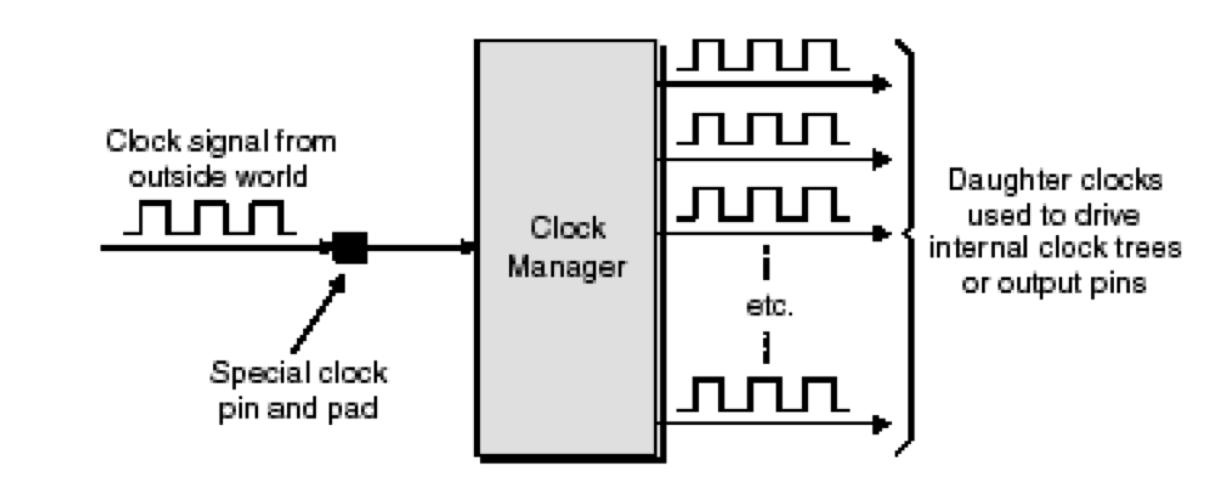
\includegraphics[width=0.5\textwidth,keepaspectratio=true]{./images/dougther}
  		\caption{Clock manager}
  		\label{fig:dclocks}
 		\end{center}
		\end{figure}

		Se tiene  una estructura \textit{clock tree} por la que se distribuye la señal de clock principal, que es ramificada para
		que alcance a todos los flip-flops. Esta estructura es así para asegurar que todos los flip-flop estén lo más cerca posible del clock y evitar el
		problema del \textit{skew}. El \textit{clock tree} es implementado usando canales separados de los de propósito general para interconectar los
		bloques (Figura ~\ref{fig:ctree}).

		\begin{figure}[h!]
 		\begin{center}
 		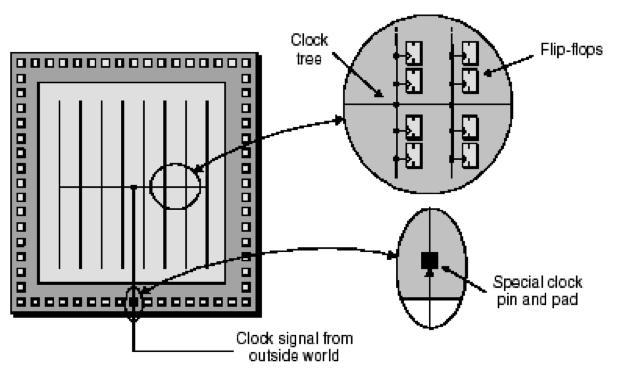
\includegraphics[width=0.5\textwidth,keepaspectratio=true]{./images/clocktree}
  		\caption{Clock tree}
  		\label{fig:ctree}
 		\end{center}
		\end{figure}

	\subsection{Tipo de tecnología} 
	Teniendo en cuenta al tipo de tecnología que utilizan las \textit{FPGAs} para almacenar sus datos de configuración, estas se pueden clasificar en
	tres tipos:

	\begin {itemize}
	\item  
	\textit {Basadas en memoria RAM estática (SRAM)}: Las \textit{FPGAs} guardan su configuración en una memoria interna de tipo SRAM. Cada vez que se
	enciende el sistema es necesario reprogramar la \textit{FPGA} con su configuración, por lo tanto es necesario almacenar esta configuración en un
	dispositivo ROM externo o descargarla desde un PC conectado a la \textit{FPGA}. Este tipo de \textit{FPGA} es la más flexible y permite utilizar
	técnicas de reconfiguración dinámica.
	\item  
	\textit{Basadas en memoria ROM}: Las \textit{FPGAs} almacenan su configuración en una memoria interna de tipo ROM, normalmente FLASH o EEPROM, siendo
	la tecnología FLASH la dominante en estos momentos. La ventaja es que al apagar la \textit{FPGA} la configuración no se pierde, por lo que no son
	necesarios componentes externos para almacenarla. Es menos flexible ya que la configuración es más lenta y no permite utilizar técnicas de
	reconfiguración dinámica.
	\item  
	\textit{Basadas en fusibles}: La configuración se almacena “quemando” fusibles durante el proceso de programación. Actualmente la tecnología más
	utilizada en estas \textit{FPGAs} es la basada en anti-fusibles(anti-fuse). La configuración queda grabada en la \textit{FPGA} de forma que no es
	posible reprogramarla, lo que elimina cualquier tipo de flexibilidad.
 	\end {itemize}

\section{Microprocesadores Softcore Reconfigurables}
	\subsection{Introducción}
	El avance en la tecnología de fabricación de VLSI (Very Large Scale Integration) a medida que se agregaron más y más transistores, y en
	consecuencia más y más funciones fueron integradas en un mismo chip, por lo tanto también las capacidades en FPGAs. Grandes diseños de sistemas
	digitales que fueron sólo para ser implementado como ASICs, luego tuvieron la opción de ser ejecutados en FPGA.
	
	El microprocesador, ya sea como un componente discreto o como parte de otra lógica en el mismo chip, es un buen candidato para ser implementado en
	FPGA. Esto introdujo un mayor potencial para la exploración del espacio de diseño haciendo que la lógica de cómputo específica sea implemetada junto
	con un microprocesador estándar. \cite{Etiqueta05}
	
	Dentro de los microprocesadores \textit{Softcore} se encuentra un grupo que apunta principalmente a la reconfiguración de hardware.
	Tres de los más grandes proveedores de FPGA: Xilinx , Altera y Lattice; ofrecen sus propios núcleos de microprocesadores RISC de 32 bits.
	Existe un grupo de núcleos \textit{Softcore} \textit{Open Source} no limitados por la tecnología. Este grupo es desarrollado por
	lo general por aficionados en comunidades \textit{Open Source}, o en algunos casos, desarrollados por entidades comerciales antes de ser \textit{Open
	Source}.
	
	Para los desarrollos dirigidos a una reconfiguración de hardware la opción de microprocesadores \textit{Softcore} de 32 bits se
 	encuentra entre los que ofrecen los proveedores de FPGA y tambien disponible sin costo dentro de las comunidades \textit{Open Source}. Sin embargo,
 	cuando se trata de ser capaz de desarrollar y vender un producto basado en estos \textit{Cores} \textit{Open Source}, hay consideraciones
 	adicionales sobre la concesión de licencias.
	
	Las verdaderas ventajas de\textit{Softcore Open Source}, tienen que ver con la apertura del diseño, y la ausencia de restricciones sobre lo que se
	puede hacer con el \textit{Core}. Con un diseño de código abierto existe la opción de personalizar la descripción RTL para implementar la
	optimización o la funcionalidad deseada.
	
	La portabilidad y la reutilización del producto final, así como su vigencia por causa del acceso al diseño escrito en lenguaje de descripción de
	hardware también es una de las grandes ventajas de \textit{Softcore Open Source}.

	\subsection{IP-Core}
	El diseño de circuitos digitales se divide normalmente en bloques funcionales, que se refieren como \textit{módulos}, o \textit{cores}. Un
	\textit{core} está formado por sub-bloques que ayudan a poner en práctica su funcionalidad. Los \textit{cores} pueden variar en tamaño hasta el
	tamaño total de un microprocesador. Un \textit{core} puede ocupar una FPGA entera al ser implementado, mientras que sólo se crea una instancia entre
	otros en una FPGA más grande o en un ASIC. Los \textit{núcleos} se describen generalmente utilizando un lenguaje de descripción de hardware (HDL) en
	un nivel de abstracción conocida como Register Transfer Level (RTL).
	
	El proceso de tomar la descripción RTL de un diseño y convertirlo en un lista de primitivas o puertas lógicas y las conexiones entre ellos, dejando
	luego que la  implementación se realice en una tecnología de destino, se conoce como \textit{síntesis}. Análogamente a la compilación de software	que
	se tiene un programa en un lenguaje de alto nivel, como C, y  es convertido a codigo maquina. El resultado de la síntesis, conocida como una
	\textit{netlist}, está en un nivel de abstracción denominado nivel de la puerta.En pocas palabras, es esta lista de conexiones que se utiliza para
	su posterior procesamiento en una configuración para FPGA o en un diseño para ASIC.
	
	Los cores pueden ser diseñados por una persona o entidad, los desarrolladores de \textit{cores} y licenciatarios varían desde particulares
	a empresas. El producto, en este caso se conoce como un \textit{IP core (Intellectual Property Core)} el diseño es la propiedad intelectual de los
	desarrolladores. 
	
		\subsubsection{Tipos de IP-Cores}

		Los \textit{IP cores} se clasifican de acuerdo a su licencia las cuales se presentan a continuación:
		
			\paragraph{Softcores}
			Son los más flexibles y se presentan para \textit{IP} en forma netlist (lista de compuertas e interconexiones) o en forma de sintetizable RTL, lo
			que los hace tecnológicamente independientes.Los \textit{cores} sintetizable se entregan en un lenguaje de descripción de hardware como Verilog o
			VHDL. Óptimos para diferentes aplicaciones, a costas de menor predictibilidad en la implementación y suelen tener un mayor costo y menor desempeño
			de procesamiento.

			\paragraph{Firmcores}
			Los cores firmes están optimizados para ser implementados en una FPGA, arquitectura o dispositivo en particular. Esta optimización puede ser
			realizada por el fabricante o por un tercero. Utilizar este tipo de IP-Cores requiere disponer de cierto nivel de conocimiento de la arquitectura,
			ya que es posible rutear señales físicas y especificar la colocación de los elementos de diseño. Un ejemplo de cores firmes es el procesador
			MicroBlaze de Xilinx.\cite{Etiqueta04}

			\paragraph{Hardcores}
			Están optimizados para una tecnología específica y no pueden ser modificados por el diseñador que los utiliza. Son manifestaciones físicas del
			diseño del core ya que tienen un layout predefinido incluido en la arquitectura. Son los mejores para aplicaciones plug\&play. Si bien son poco
			flexibles, portables y configurables, son muy predictibles (el timing es fijo) y fiables una vez implementados.

		\subsubsection{Clasificación de acuerdo con la integración}
		El aumento de recursos de las FPGAs junto con la amplia disponibilidad de bloques IP ha hecho posible la integración de sistemas completos en la
		propia FPGA y la aparición de una nueva terminología para clasificarlos. Algunos de los términos que se usan para designar este tipo de sistemas
		son:
		\begin {itemize}
		\item 
		\textit{System on Chip (SoC)}:
 		Circuito integrado formado por diversos módulos VLSI con distinta funcionalidad que interconectados entre sí ofrecen una funcionalidad específica
 		para una aplicación.
		\item 
		\textit{System-on-Programable-Chip (SoPC)}: Se aplica este término específicamente cuando el dispositivo utilizado para realizar el SoC es
		reconfigurable.
		\item 
		\textit{Configurable-System-on-Chip (CSoC)}:Mediante este término se definen los sistemas SoC en los que se hace uso de la capacidad de
		reconfiguración de los mismos para aplicaciones de computación reconfigurable. Pueden incluirse bajo la denominación CSoC tanto los sistemas que
		admiten diferentes configuraciones estáticas según ciertos condicionantes, como los que utilizan la reconfiguración parcial dinámica para modificar
		en tiempo de ejecución una sección hardware.
		\item 
		\textit{Multiprocessor-Configurable-System-on-Chip (MCSoC)}: Se aplica esta definición a los sistemas CSoC que incluyen varias unidades procesador
		funcionando de forma simultánea.
 		\end {itemize}

 % FPGA y Micro Soft Cores
\newpage
%\chapter{Software OpenSource y Libre}
\section{Introdución} 
	\par
	El software \textit{Open Source} (Fuente Abierta) podría traducirse como " Código fuente abierto ", es un tipo particular de software que ofrece al
	usuario la posibilidad de conocer el código fuente para su estudio o modificación. No sólo hace referencia al libre acceso al código fuente, las
	condiciones de distribución de un programa \textit{Open Source} deben cumplir una serie de criterios, que a continuación se exponen. El propósito de
	establecer una definición oficial de \textit{Open Source} es establecer que esos criterios contengan la esencia de lo que los programadores quieren que
	signifique: que aseguren que los programas distribuidos con " Licencia Open Source " estarán disponibles para su continua revisión y mejora para que
	alcancen niveles de fiabilidad que no pueda conseguir ningún programa comercial cerrado sin discriminar a personas ni a grupos de personas que
	quiera utilizarlo. Es un término ambiguo, el acuerdo sobre la definición está en el documento llamado Open Source Definition (OSD), publicado por la
	Open Source Initiative (OSI). La OSD da grandes libertades a la hora de relicenciar software, lo que no sucede con otras licencias de código
	abierto. En particular la OSD permite " mezclar " software privativo con software \textit{Open Source}.
	\vspace{0.5cm}
	\par
	La Fundación para el Software Libre (FSF) determina claramente, qué se tiene que cumplir sobre el software para que pueda ser considerado
	\textit{libre} \cite{Etiqueta07}. El software \textit{libre} se refiere a la libertad de los usuarios para ejecutar, copiar, distribuir, estudiar,
	cambiar y mejorar el software. El vocablo \textit{free} en inglés significa: gratis y/o libre. Por ello el término ha ocasionado confusiones dándose
	a entender, equivocadamente, que el software libre es gratuito o regalado. No es una cuestión de presencia o ausencia de costo, puesto que el
	software libre no significa que no pueda ser comercial.
	\vspace{0.5cm}
	\par
	Richard Stallman fundó la FSF en 1985 para promover la libertad del usuario y defender los derechos de todo el software libre \cite{Etiqueta14}. La
	FSF patrocina el proyecto GNU. El software libre permite al usuario el ejercicio de cuatro libertades básicas:
	\begin {itemize}
	\item
 	\textit{Libertad 0} El software \textit{libre} permite estudiar cómo funciona y adaptarlo a las necesidades de quién lo use. Tener acceso a
 	su código fuente posibilita, entre otras cosas, descubrir funciones ocúltas, averiguar como se realiza determinada tarea, descubrir qué
 	posibilidades tiene, etc. Al adaptar el programa a las necesidades del usuario pueden suprimirse partes que no le interesen, agregar otras partes
 	que considere importantes copiar una parte que realiza una tarea y/o adicinarla a otro programa, etc.
	\item
	\textit{Libertad 1} El software, sus copias y las modificaciones se pueden distribuir libremente, lo que significa poseer la libertad de redistribuir
	el programa, gratis o con algún costo, ya sea por mail, FTP, o en CD, redistibuyéndolo a una persona o a varias, a una persona que vive en otro país,
	etc.
	\item 
	\textit{Libertad 2} Es posible mejorarlo y hacer pública esas mejoras. La libretad de hacer un programa mejor, implica que se puede hacer menores los
	requerimientos de hardware para funcionar, que tenga mayores prestaciones, que sus requerimientos no sean tan altos, que tenga menos errores, etc. El
	poder liberar las mejoras al público quiere decir que si se realiza una mejora que permita un requerimiento menor de hardware, o que haga que ocupe
	menos espacio, se puede redistribuir ese programa mejorado o simplemente proponer la mejora en lugar público (un foro de noticias, una lista de
	correo, un sitio web, un FTP, un canal de chat).
	\item 
	\textit{Libertad 3} El usuario al poseer el código fuente tiene poder de decisión, ya que podrá elegir quién puede modificar los programas que ha
	adquirido para mejorarlos (o bien mejorarlos el mismo). Es decir, esto permite que no exista un monopolio, porque en el caso de que un software sea
	discontinuado el usuario podrá nuevamente (al poseer el código) elegir a un desarrollador para continuar utilizando el software que fue
	discontinuado. Además el usuario no estará completamente a merced de tener que renovar su hardware y software constantemente según ocurre a menudo
	con las políticas de las empresas que producen software privativo y también será libre de vender o redistribuir software libre.
 	\end {itemize}
 	\vspace{0.5cm}
	\par
	El termino Free and Open Source Software (FOSS) se utiliza para referirse al software que se adhiere al OSD y FSF. El software libre y de código
	abierto es una sociedad inclusiva, el término abarca tanto el software libre y software de código abierto a pesar de describir modelos de desarrollo
	similares, tienen diferentes culturas y filosofías.
	\vspace{0.5cm}
	\par
	Mediante la \textit{licencia} un autor permite el uso de su creación a otras personas, de la manera que él cree aceptable. En ese sentido
	la \textit{licencia} es el instrumento que regula las maneras en que el usuario puede utilizar el software. Una \textit{licencia} de software es un
	contrato que determina en qué condiciones el usuario puede utilizar el programa informático y qué obligaciones adquiere para su uso. Cuando se
	instala un programa informático, o a veces, incluso, por el simple hecho de abrir el sobre que lo contiene, se esta aceptando las condiciones de su
	\textit{licencia} de software.
	\vspace{0.5cm}
	\par	
	Cuando IBM comenzó la venta de computadoras a gran escala en la década de 1960, el software venía incluido con su código fuente. Una década más
	tarde, sin embargo, comenzaron a " desagregar "  el código fuente, convirtiéndose en algo habitual para los fabricantes, este hecho limitó el uso del
	código fuente a sus competidores, sin embargo, también eliminó la capacidad de modificar libremente el código y compartirlo. \cite{Etiqueta08}.
	\vspace{0.5cm}
	\par	
	La \textit{licencia} División de Software de Berkeley (BSD) y la GNU General Public License (GNU GPL) son dos de las primeras licencias de código
	\textit{libre}. Ambas proporcionan la libertad de usar software de código abierto para cualquier propósito y permitir la modificación y la
	distribución de su código fuente sin tener que pagar regalías. Un punto significativo de diferencia entre las \textit{licencia} BSD y GPL es que la
	primera permite el uso del código fuente en software no libre.
	\vspace{0.5cm}
	\par	
	La GNU GPL se conoce como una \textit{licencia viral}, donde cualquier desarrollo que se haga bajo el uso de código licenciado bajo la GNU GPL debe
	ser entonces licenciado bajo la GNU GPL o cualquier \textit{licencia} autorizada por la FSF. En pocas palabras, una condición de uso del código
	licenciado bajo GPL es que su diseño se debe tener bajo la licencia  GPL o una licencia compatible. Las licencias que se consideran compatibles con
	la GPL por la FSF son generalmente similares en las libertades que garantiza el software \textit{libre}.
	\vspace{0.5cm}
	\par	
	La licencia BSD modificada es básicamente la misma que la original sin la clausula de publicidad. De acuerdo con dicha cláusula, todo el material de
	publicidad en el cual se menciona características o la utilización de este software tenia que mostrar el siguiente asentimiento: " Este producto
	incluye software desarrollado por la Universidad de California, Berkeley y sus contribuyentes ". Esta cláusula de publicidad no permitía que fuera
	compatible con la licencia GPL pero a partir de su versión 2.0 fue eliminada y la licencia pasó a ser compatible con la GPL.
	\vspace{0.5cm}
	\par	
	En la GNU se estipula que el código modificado debe estar disponible, y que cualquier desarrollo que utilice código bajo esta licencia tiene también
	que estar bajo la GNU GPL. Aunque, esto no es diferente a cualquier licencia comercial, donde el código fuente creado o modificado por los empleados
	de una empresa queda bajo la licencia exclusiva de la empresa. En el caso de la licencia de GNU, sin embargo, los usuarios están obligados a mantener
	sus diseños abiertos y libres, de la misma manera que los empleados estan obligados a mantener su código propietario en secreto para cualquiera que
	no sea de la empresa.
	\vspace{0.5cm}
	\par	
	Otro punto de controversia es el uso combinado del código fuente donde cada uno esta bajo una licencia diferente, dando lugar al concepto de
	\textit{compatibilidad de la licencia}. En el caso de que un desarrollo utilizara una librería bajo licencia GPL, la GNU GPL especifica que se puede
	utilizar tal librería si el diseño que la requiere este también bajo la licencia GPL. El uso de librerías precompiladas es muy común en aplicaciones.
	En el caso de que la librería se encuentra bajo licencia GPL, cualquier programa que haga uso de ella (también conocido como la creación de un
	\textit{link} a la librería) debe también estar bajo la GPL. Sin embargo, la inclusión en una aplicación compilada de un binario GPL (conocido como
	\textit{vinculación estática}) no es realmente un problema, esto es equivalente a incluir el código fuente completo y generar mediante la
	compilación de todo el código un binario ejecutable. El debate es sobre la \textit{vinculación dinámica}. Esto implica el uso de una librería de
	software precompilada que reside en memoria (no dentro de una aplicación compilada) cuando se ejecuta una aplicación. El hecho que un programa que 
	vincula dinámicamente a una librería es considerado un trabajo derivado es un tema de debate. El proyecto GNU considera esas aplicaciones como
	derivadas y les obliga a cumplir con los requisitos de la licencia GNU GPL.
	\vspace{0.5cm}
	\par	
 	Una solución para aquellos que deseen escribir bibliotecas sin ajustarse a la interpretación estricta de trabajo derivado, fue
 	propuesta por GNU en su Licencia de Uso General Menor (LGPL). Se trata de un trade-off, lo que permite desmostrar que la tecnología licenciada bajo
 	el Proyecto GNU es de alta calidad, fomentando así la participación de las personas en el proyecto, al tiempo que conserva algo de sus requisitos
 	de la libertad. El proyecto GNU, sin embargo, prefiere que los desarrolladores liberen bibliotecas bajo la GPL, lo que obliga a quienes las
 	utilizan a contribuir con su trabajo a una parte del proyecto de GNU.
	
	
%%%%%% HASTA ACÁ    %%%%%	
	
	\vspace{0.5cm}
	\par	
	Una solución para aquellos que deseen escribir librería y no tienen la interpretación más estricta de los trabajos derivados se aplica la propuesta
 	del Proyecto GNU la Licencia Pública General Reducida de GNU, o más conocida por su nombre en inglés GNU Lesser General Public License (GNU LGPL). Está
 	licencia permisiva se aplica a cualquier programa o trabajo que contenga una nota puesta por el propietario de los derechos del trabajo,
 	estableciendo que su trabajo puede ser distribuido bajo los términos de la licencia LGPL. El "software" utilizado en lo subsecuente, se refiere a cualquier programa o trabajo original y el "trabajo basado en el software" significa también el programa o cualquier trabajo derivado del mismo bajo la ley de derechos de autor. Es decir, un trabajo que contenga el Programa o alguna porción de él, ya sea íntegra o con modificaciones o traducciones a otros idiomas.Otras actividades que no sean copia, distribución o modificación no están cubiertas en esta licencia y están fuera de su alcance. El acto de ejecutar el programa no está restringido, y la salida de información del programa está cubierta sólo si su contenido constituye un trabajo basado en el Programa (es independiente de si fue resultado de ejecutar el programa). Si esto es cierto o no, depende de la función del programa.\cite{Etiqueta03} 


	Estas diferencias de opinión con respecto a lo que constituye un trabajo derivado, y la ambigüedad en torno a otros
	aspectos de la concesión de licencias de código abierto podría tener consecuencias para campos como el diseño de hardware, lo que se discutirá en una
	sección posterior.


	 La principal diferencia de opinión, sin embargo, se deriva del hecho de que la FSF desea hacer imposible que el software
	propietario  pueda utilizar software liberado bajo la GNU GPL. La FSF argumenta que los que no están dispuesto a permitir que otras personas vean o
	modifiquen libremente su código aprovechen de los que sí lo permiten. Otras licencias de código abierto, sin embargo ,son más permisivas en la
	utilización de sus diseños como por ejemplo en el código fuente de las librerías, en aplicaciones propietarias.El objetivo del Proyecto GNU de implementar 
	un sistema operativo completamente libre y gratuito, avanzo a buen ritmo en la década del 90, pero le faltaba la llave de componentes del nivel más bajo.


	El núcleo o kernel de Linux iniciado por Linus Torvalds, fue liberado para poder ser modificado libremente en 1991. La licencia inicial, no fue exactamente una
	licencia de software \textit{libre}, sin embargo la version 0.12 lanzada en febrero de 1992, fue licenciada nuevamente por Torvalds bajo los términos de la
	licencia GPL GNU. Así como Unix en su tiempo, el núcleo de Torvalds atrajo la atención de programadores voluntarios.Hasta este punto, la falta de núcleo del proyecto GNU				significaba la no existencia de un sistema operativo libre completo. El desarrollo del núcleo de					
	Linux Torvalds lleno este último hueco. La combinación del casi terminado sistema operativo GNU y el núcleo Linux resultó en el primer sistema
	operativo completo de software\textit{libre}.El GNU/Linux (o simplemente Linux) continúa siendo software libre desarrollado por programadores voluntarios, pero también 				muchas compañías ofrecen productos personalizados basados en el núcleo Linux, así como distribuciones con soporte comercial.


	Otros ejemplos de proyecto de código abierto exitosos y ampliamente adoptados son, el servidor web Apache, el paquete \url{OpenOffice.org} y el proyecto Mozilla. A pesar de 			que estos dos últimos no eran originariamente de código abierto, el lanzamiento de su código fuente bajo licencias de código abierto fue significativa y continúan en la 					actualidad.
	
	

	Tras la adopción creciente de software de código abierto en la década del 90, la organización OSI fue iniciada por desarrolladores de software que propusieron que el 					software\textit{libre} (como lo fue comúnmente conocido en ese entonces) tenía un lugar en la industria comercial. El éxito del modelo sorprendió a mucha personas y demostró 		que era un modelo de desarrollo viable. A medida que la popularidad y la utilidad de Internet fue creciendo, también lo hicieron las comunidades de código abierto por 					diferentes causas; la atracción y la comunicación que produce internet en personas interesadas en el desarrollo de código abierto, proporciono el inicio para las grandes
	comunidades de código abierto, lo que ha dado como resultado un sinnúmero de comunidades y grupos que contribuyen al desarrollo de código abierto.


	EL sitio web\textit{OpenCores}con sus comienzos en el año 2000, proporciona un sitio para la comunidad de hardware de código abierto.
 	Fue una de las primeras comunidades de desarrollo de hardware y actualmente la mas grande, con más de cien mil usuarios y cerca de mil proyectos. Donde su
	principal objetivo es diseñar y publicar diseños de núcleos bajo una licencia de hardware de código abierto siguiendo el modelo de Licencia LGPL usada para el software.
	Se comprometen con el ideal de libre disposición, uso y reutilización de hardware de código abierto.\cite{Etiqueta10}

	\subsection{Código Abierto adoptado para la Industria}

	Dentro del software de código abierto se tienen alternativas como: software multimedia, productividad de oficina, herramientas de
	gráficos, sistemas operativos y de comunicaciones, por lo general libres para descargar y utilizarlos. Los gobiernos y las grandes empresas están aprovechando cada 			vez más el software de código abierto que existe y se están convirtiendo en importantes contribuyentes a los proyectos del software que adoptan. Las tendencias recientes han hecho mucho para disipar la imagen de solitarios desarrolladores de código abierto como los únicos contribuyentes de trabajos. Al estar las entidades comerciales aumentando la adopción y utilización de los proyectos de software libre,  se están convirtiendo en los contribuyentes más frecuentes. Actualmente el kernel de Linux tiene la mayor parte de sus contribuciones de código de entidades comerciales, ya sea porque están trabajando con el núcleo Linux en sus productos o porque desean asegurar el apoyo a su hardware en el kernel tales como Intel,  IBM y AMD. Lo mismo pasa para proyectos como Apache y MySQL.

La gran cantidad de software de código abierto disponible ofrece la adopción de licencias FOSS con la posibilidad de elegir entre: la publicación del trabajo derivado, el desarrollo de una solución interna o la compra de una solución propietaria manteniendo el código en privado.

 Las entidades comerciales interesadas en mantener sus plataformas en buenas condiciones son en gran parte las que ofrecen mayor soporte y desarrollo a herramientas de programación como el compilador GCC y binutils del proyecto GNU. El desarrollo de las herramientas de software de código abierto es impulsado por GNU brindando soporte a diferentes plataformas con el fin de fomentar el uso de un compilador-optimizador de clase global, que atraiga a desarrolladores entregando herramientas que funcionen en diferentes arquitecturas. 

El inminente aumento comercial del software de código abierto trae como consecuencia que las empresas aporten recursos a estos proyectos en lugar del desarrollo y 			mantenimiento de su propio conjunto de compiladores y herramientas, por ejemplo en el caso del GCC. Uno de los objetivos del código abierto es proporcionar una base de software donde los desarrolladores se encuentren cómodos para adoptarlo y como consecuencia el crecimiento del software existente producto de la publicación de sus trabajos derivados, evitando la tarea de empezar a desarrollar desde cero o comprar una solución propietaria. Estas son algunas de las motivaciones para la adopción y contribución de código abierto, podrían ser muchas más y variadas eso dependerá de la funcionalidad del proyecto. A pesar de su éxito con el software en el hardware no tuvo el mismo éxito los motivos se desarrollan más adelante.

%%%%%% HASTA ACÁ    %%%%%	
		\subsubsection{Mas motivación para la adopción para el desarrollo OpenSource}
Una de las motivaciones para el desarrollo de código abierto desde el punto de vista comercial,  proviene de la capacidad de proporcionar y cobrar por algún tipo de servicio extra del proyecto de código abierto.A pesar que el IP este disponible públicamente, implementar o personalizar el proyecto normalmente requiere experiencia en el correspondiente disciplina y con el proyecto en particular. Las empresas que adoptan y mantien una solución de código abierto por lo general tienen sólo el costo de los conocimientos necesarios para hacerlo, sin tener que pagar regalías o licencias adicionales.  

En la actualidad hay alternativas de código abierto a los sistemas de software propietarios de IT (Tecnología de la información),  los desarrolladores de código abierto renuncian a ciertos derechos sobre la IP, la que gran parte no era su propia idea o considera innovadora, para comenzar a ganar de otra forma como por ejemplo realizando servicios de mantenimiento o adaptación de acuerdo a las requerimientos necesarios en el proyecto derivado.

A pesar de que el software de código fuente abierto no es tradicionalmente un generador continuo de productos innovación no se opone a que sea la estrategia de desarrollo elegida para una tecnología innovadora. Cualquier diseño innovador opensource suele tener retornos valiosos para la inversión necesaria para llevarla a cabo. Sin embargo, con alternativas de código abierto que brotan de forma relativamente rápida, su ventaja no puede durar por mucho tiempo producto de que otros toman nota de lo que han hecho desarrollos innovadores y si vale la pena el producto, utilizan la soluciones de código abierto. Esto  Puede llegar a ser una opción interesante para los desarrolladores que emplean el desarrollo de código abierto para empezar con una base lo que trea como consecuencia el ahorro de tiempo para el desarrolladar del producto derivado, con la ventaja  de poder competir frente a  implementaciones propietarias, con la capacitad de proporcionar soporte técnico a largo plazo para una aplicación. Esto es un buen método, donde inicialmente el producto está autorizado por una parte y al liberar  el código fuente permite a otros desarrolladores mejorar el proyecto.

Como el ciclo de vida de un producto llega a su fin , puede ser ventajoso para software privativos liberar el código fuente para permitir a cualquier usuario con el conocimiento que requiere poder darle soluciones los problemas derivados de las actualizaciones inevitable de las plataformas que se producen . 

Todavía hay un problema aquí, sin embargo, como la implementación propietaria
mantiene su dominio, mientras que no se aparezcan una fuente de código abierto equivalente, el diseñador por lo general no elige liberar el código tomando entonces el riesgo de que aparezca un aplicación diferente con funciones equivalentes y gane más popularidad,  y por lo tanto la idea del diseñador original sigue, pero no su capacidad para proporcionar apoyo a la misma.

Esta breve mirada a la situación actual de código abierto ha indicado que el código abierto
se ha convertido en una fuerza a tener en cuenta en el mundo del software, pero este no es el caso en la actualidad para el desarrollo de hardware de código abierto.
 A medida que la cantidad de código abierto disponible aumenta, y la comprensión de los márgenes de aproximación , lo hará
seguramente continuará para demostrar que es un enfoque valioso para el desarrollo de
la tecnología .

As the wealth of available open source designs increases, and the understanding of the approach spreads, it will surely continue to prove itself as a worthwhile approach to the development of technology.
\subsubsection{Desventajas de la adopción del OpenSource}

Son muchos los que no están de acuerdo con el desarrollo de código abierto en la actualidad a pesar del gran aumento en su popularidad y uso. El software o hardware privativo puede ser desplazado del mercado por una alternativa no privativa, sin costo. Los que obviamente van a estar en desacuerdo son las entidades que se encuentren amenazadas por una alternativa lo suficientemente innovadora que provoque una disminución en sus ganancias. Una alternativa para los menos favorecidos es usar el código abierto existente que generalmente no es suficientemente innovador y mejorarlo. Permitiendoles competir con cualquier producto del mercado. De este modo los desarrolladores adquieren conocimientos ademas de ahorrar tiempo y desarrollaron un negocio, proporcionando un servicio de apoyo para la suma de un proyecto mejorado.


El inconveniente de mostrar el código del proyecto mejorado es que los desarrolladores exponen sus técnicas innovadoras y obtiene una ganancia como se acostumbra en los productos de software propietario. Sin embargo, esto es compensado por la reducción de la inversión en el desarrollo de su producto (una gran proporción de
la infraestructura de apoyo adoptada de implementación de código abierto) y su mejora sobre el proyecto de código abierto recientemente mejorada atrae a otros contribuyentes que deciden trabajar con el proyecto.

En los proyectos de código abierto uno de los principales problemas es la dificultad de ser implementados. Para los principiantes, contribuir a un proyecto de código abierto puede
ser significativo y esta es otra crítica común de desarrollo de código abierto.



%%%%%%%%%%%%%%%%%%%%%%%%%
Es cierto que las implementaciones de código abierto varían enormemente
en calidad y funcionalidad y esto se debe normalmente a una base colaborador limitada que está implementando sólo lo suficiente para que funcione para su aplicación. 

Para el no iniciados, las barreras de entrada para contribuir a un proyecto de código abierto puede
ser significativo y esta es otra crítica común de desarrollo de código abierto.
Los proyectos más grandes y mejor gestionadas, por lo general no tienen estos problemas a medida que adoptan una
enfoque más profesional para el desarrollo, y por lo general tienen los tecnicos en la mantención de tiempo completo
que se encargará de todas las nuevas características no causan errores en otros lugares, o el retroceso
la funcionalidad del proyecto.

Hay argumentos que OS impide la competicion porque reduce las chances de los desarrolladores propietarios dado que los OS suelen ser mas usados dado que es gratis. Entonces es argumentado que la innovacion esta estancada ya que las compañias pequeñas no pueden meterse en las aplicaciones OS ni en los productos pagos, que antes hubiesen tenido oportunidad de mejorar.

Other standard complaints about open source projects are in regard to the quality
of implementation. It is true that open source implementations do vary greatly
in quality and functionality and this is typically due to a limited contributor base
that is implementing only enough so that it works for their application. For the
uninitiated, the barriers to entry for contributing to an open source project can
be significant and this is another common criticism of open source development.
Larger, better managed projects, typically do not have these issues as they adopt a
more professional approach to the development, and typically have full time maintainers
who will ensure any new features do not cause errors elsewhere, or regress
the project’s functionality. However, on smaller projects, with only a handful of
contributors, unfinished features can be common. On the other hand as the design
is completely open, and although there’s a relatively steep learning curve, missing
features can be added and problems can be fixed by anyone, as they’re required.
There’s no doubting some very useful software has been written and contributed
to open source software projects, however open source should not be seen as an innovative
force, rather a step on the way to further commoditising a technology.

Entrepreneurship and the profit motive typically drive the high risk and high innovation
firms which are involved in cutting edge technology implementation. The
whole premise of the GNU Project (GNU is a recursive acronym for “GNU is Not
UNIX”) was to develop, in essence, a free, open source copy of UNIX applications
and operating system. This was not innovation, rather imitation but with a different
goal for the resulting work. The Linux kernel was begun for similar reasons.
It demonstrated engineering capability but not ingenuity, at least not at that time.
It is not true to say that what has been developed in and around those projects
doesn’t have its innovative elements. It is one thing to wish to re-implement an
existing application for largely academic purposes, and another to wish to invest
large amounts of time and money to develop a new concept wishing to see a return
based on the innovation, rather than the accessibility, of the design.





\section {OpenSource}

La apertura del código de la propiedad intelectual desarrollada para el proyecto OpenRISC, y otros en OpenCores, ha sido a la vez un obstáculo y una ayuda, ya que pone al desnudo el estado del desarrollo, pero es útil, ya que permite que cualquiera pueda participar en el continuo desarrollo de núcleos. Esta subsección discutirá los pros y los contras de la fuente abierta enfoque.

		\subsection{No verificado y No populares}

A pesar del uso y la aceptación del software desarrollado bajo licencia de código abierto, los proyectos RTL de código abierto no han recibido el mismo tipo de interés o la participación de las empresas más grandes de IP. 

Un problema es para las personas que desarrollan IP destinados para su implementación en ASIC, es la falta de un conjunto de herramientas de verificación para los IP de codigo abierto, y por lo tanto la incapacidad para verificar rápidamente la funcionalidad de un core, esto es inaceptable dado el elevado costo de la corrección de errores. Se podria sugerir la inclusión obligatoria de una herramienta de verificacióne con el core, sin embargo, las herramientas estándares de verificación que se encuentran disponibles en la industria son de entidades propietarias y tienen un elevado costo y pueden variar de un proveedor a otro. 

Es sorprendente que no existen herramientas de verificación de código abierto en la industria todavía, esto pone un serio obstáculo para la entrada al mercado de desarrolladores IP por el importante costo del conjunto de herramientas de Entorno de desarrllo integrado (EDA) capaces de realizar la verificación.A falta de las opciones de EDA de código abierto continuarán limitando las aplicaciones de estos núcleos opensource, y para minimizar el riesgo las implementaciones se realizaran en dispositivos como las FPGAs donde generalmente se pueden hacer cambios  del RTL con un bajo costo 
 

	\subsection{¿Cual es su objetivo? }


Una barrera para el desarrollo de hardware de código abierto que no la tiene el desarrollo de software, es el requerimiento de la plataforma donde implementar el diseño del prototipo,así como herramientas  de progrmacion y depuración gratuitas . Estas plataformas, típicamente placas que contienen múltiples periféricos ICs basadas en una FPGA, así como la depuración de hardware y programación no son independientes de un proveedor. A esto se suman la complejidad de las herramientas de programación de los proveedores para la FPGA, así como el desarrollo de hardware con una curva de aprendizaje relativamente empinada que perjudica a los principiantes.
También  la utilidad de cualquier diseño de hardware que se podría implementar en una FPGA está limitada por el hecho de que se realiza a un nivel muy bajo de abstracción, y para lograr un resultado positivo "útil" para los experimentador o aficionado, por lo general requiere un gran trabajo a través de muchos niveles de abstracción para lograr algo que sea fácilmente utilizable a partir de una interfaz de una PC. 

Un ejemplo podría ser el desarrollo de un core para que realice transacciones de I/O de un sensor, para proporcionar información a una aplicación por ejemplo que controle la temperatura en un espacio determinado. Esto requeriría el desarrollo y prueba del modelo de hardware y la implementación en FPGA . Asumiendo que es un microprocesador el que se encuentra corriendo sobre la FPGA, dando servicios de red a través de un sistema operativo de tiempo real (RTOS), este módulo personalizado debería requerir el desarrollo de una capa de software, lo que significa la necesidad de un driver para que permita al sistema operativo en tiempo real interaccionar con el periférico, haciendo una abstracción del hardware y proporcionando una interfaz para usarlo. El sistema operativo en tiempo real se conecta con la aplicación que se ejecuta en el microprocesador de la FPGA para proporcionan lo datos a través del enlace de red, solo entonces los datos de este sensor se encontraran disponibles para la aplicación de nivel superior. This is just one example where, quite probably the designer might have chosen a solution that uses a standard bus, however there’s often cases for custom controller or interface cores in FPGAs to provide
access to legacy, or very-new or esoteric bus standards, and highlights the extra work required beyond writing RTL to provide the physical interface.
Viendo la cantidad de desarrollo y pruebas requeridas para poner en práctica estas soluciones, es fácil sentirse abrumado por la cantidad de trabajo necesario para completar una tarea tan aparentemente trivial.

Comparando esto con adoptar una programa opensource, que consiste en la descargar de una código fuente, compilarlo y ejecutalo en su computadora. Donde La aplicación puede ser ejecutada en el  host para comprobar la funcionalidad y la mayor parde del ciclo de desarrollo termina allí. Las diferencias son el acceso inherentes a la plataforma de desarrollo (el host), las herramientas de desarrollo mucho mas simples (gcc, make en el sistema host) el ciclo de desarrollo, pruebas más cortas y más fácil (que se ejecuta en el equipo host a través de un shell.)

A medida que mas proyectos opnesource son desarrollados y los sistemas de desarrollo sean mas ágiles, se puede esperar que estas barreras para los desarrolladores de diseño de hardware opensource puedan ser superadas. En los principios del del desarrollo de software opensource parecían igual de complicados. Se espera que con el tiempo y el aumento de participantes el hardware de código abierto alcance el mismo exito.En ese momento, los diseños serán tan grandes que no cabrán en los dispositivos programables actuales. La reconfigurabilidad será un elemento imprescindible. Las fronteras entre el hardware y el software se harán cada vez más difusas. El deseo, casi utópico, es lograr correr un kernel Linux hardware basándose en las posibilidades que nos ofrece la reconfigurabilidad. 
	

\section{Licencias}

Una cuestión que queda por resolver es el de la concesión de licencias para el diseño de hardware de código abierto. El proyecto OpenRISC utiliza licencias públicas del proyecto GNU. Estos refieren específicamente a software, y no se sabe lo bien que se aplican a hardware.
El sitio web del proyecto GNU contiene una sección con preguntas frecuentes (FAQ) que se ocupa de esta consulta. Afirma lo siguiente.

\textit{Cualquier material que puede ser licenciado con derechos de autor puede ser licenciado bajo la GPL.
GPLv3 también se puede utilizar para materiales de licencia cubiertos por otras leyes copyrightlike, como máscaras de semiconductores. Así, por ejemplo, puede liberar un dibujo de un diseño de hardware bajo la GPL. Sin embargo, si
alguien utilizó esa información para crear hardware físico, que lo harían
no tienen obligaciones de la licencia al distribuir o vender el dispositivo: se
queda fuera del ámbito del derecho de autor y por lo tanto la propia GPL.}

Esto no es claro para los diseños específicos para FPGA o código, incluso RTL, ya que puede terminar como un conjunto de máscaras, o puede terminar como un flujo de bits binario para configuración de una FPGA.
Una indicación de la naciente idea de desarrollo de hardware de código abierto proviene de la publicación reciente (febrero de 2011) de un conjunto de principios para los participantes de la comunidad de hardware de código abierto. El siguiente es el código abierto Hardware (OSHW) Declaración de Principios 1.0 de FreedomDefined.org.

\textit{El Hardware de código abierto cuyo diseño está a disposición del público
por lo que cualquier persona puede estudiar, modificar, distribuir, poner, y vender el
diseño o hardware basado en ese diseño. La fuente de hardware, el diseño
del que está hecho, está disponible en el formato preferido para realizar
modificaciones a el mismo. Idealmente, el hardware de código abierto utiliza fácilmente los componetes y materiales disponible, procesos estándares, una infraestructura abierta, sin restricciones
contenida, herramientas de diseño y de código abierto para maximizar la capacidad
de las personas para hacer y usar el hardware} \cite{Etiqueta11}

Estas publicaciones proporcionan un punto de referencia para saber si el diseño puede estar bajo licencia "open source hardware".
El FreedomDefined.org es una lista con principios que específicade  fuente y  documentación, trabajos derivados y las limitaciones de la licencias. Se espera de acuerdo con estos principios, que todo el material este disponible como código fuente y la documentación para el diseño. Cualquier trabajos derivados o modificado deba estar disponible. 
Cualquier licencia de hardware de código abierto se puede utilizar para restringir (o en este caso, de forma deliberada sin restringir)los planes de un diseño, pero no el uso del dispositivo fabricado. Estos son conceptos que se encuentran a menudo en las licencias de software de código abierto, pero de nuevo, no es tan claro como se aplica en el casos del diseño del hardware de código abierto como es para el software. 

Por ahora, la primera licencia de hardware de código abierto es la  Amateur Packet Radio Licencia Open Hardware Tucson ( TAPR OHL). Los autores OHL TAPR identifican el problema con las licencias de software existentes, si bien los derechos de autor protegen la documentación de copias, modificaciones y distribuciones, que tiene poco que ver con el derecho de hacer , distribuir o usar un producto basado en la documentación \cite{Etiqueta12}.
Su licencia identifica patentes como un problema, pero afirma que quienes se beneficien de la OHL no podran
presentar una demanda alegando que el diseño infringen sus patentes u otra propiedad intelectual.
How open source hardware licenses and patent law will be compatible with regards to handling infringement is yet to be seen
En consecuencia, la TAPR OHL ha sido adoptada por un puñado de aficionados y para los intereses de empresas comerciales. Ha recibido críticas
del Instituto de Código Abierto (OSI) en la adopción de un significado diferente de la  palabra " distribución " que se suele utilizar en sus licencias, y por lo tanto no tiene un amplio apoyo entre los promovedores de código abierto\cite{Etiqueta13}. 
Sin embargo, es posibles que licencias alternativas de hardware de código abierto surjan para adaptarse a necesidades.
Para el proyecto OpenRISC hay un equilibrio para afrontar la adopción entre una licencia que es demasiado liberal, y por lo tanto menos probable que resulte en la contribución a la comunidad de desarrollo, y una licencia que fomenta mas el desarrollo de código abierto, pero se considera entonces demasiado restrictiva con respecto a la utilización de codigo abierto IP con una IP patentada.

Por un lado, hay un deseo de aumentar la participación en el desarrollo de hardware de código abierto en general, y específicamente en el proyecto OpenRISC MinSoc y OrpSoc,para aumentar el conjunto de trabajos disponibles, esto se puede lograr utilizando un licencia viral como lo es la GNU GPL (considerando la síntesis del codigo RTL como un proceso de compilación estatica). 



For the OpenRISC project there is a balance to strike between adopting a license
that is either too liberal, and thus less likely to result in contribution back to
the development community, and a license that encourages more open source development
but is then deemed too restrictive with regard to the use of open source
IP with proprietary IP. On the one hand, there is a desire to increase the participation
in open source hardware development in general, and in the OpenRISC
project specifically, and to increase the body of available work, which a viral license
along the lines of the GNU GPL (where synthesis is considered equivalent to static
linking) can achieve. On the other hand the use of the work in largely-proprietary
designs by ASIC houses is desirable as it helps prove the IP’s worth, and so a license
permitting the use of open source IP along side proprietary IP is desirable.
For the OpenRISC’s RTL implementation, the OR1200, the non-viral GNU Lesser
(L)GPL license has been used and, although the instantiation of an RTL IP block
in a “hardware” design is not dealt with specifically in the (L)GPL, it is the latter
(more liberal) licensing approach that has been taken for the OpenRISC project
thus far.
However, perhaps this factor has, too, contributed to the relatively low level
of community participation thus far in the OpenRISC project. Comparatively,
the early stages of the open source software movement saw a lot of code released
under the GPL, which ensured all other code used with it came under a similarly
“restrictive”, viral license, and ensured a large body of code was released into the
public domain. However, not all open source software was released under these viral
licenses, with the BSD and MIT licenses being less restrictive with enforcing the
freedom of the user.

\section{OpenRisc}

Como se dijo anteriormente en el debate sobre la tecnología de código abierto por lo general los modelos de desarrollo de código abierto no son imnovadores.
 La mayor parte de los proyectos de software libre tienen como objetivo utilizar recursos ya existentes y bien conocidos de manera que permitan la apertura y eliminación de restricciones que se encuentran en otra implementaciones propietarias. Esta es la duda en el caso de la OpenRISC proyecto. Es en gran medida tomando ideas que ya son bien conocidos y comoditizados
y la creación de una versión con más libertad para el usuario final. Había muy poco, si
nada, innovador en la especificación arquitectónica OR1K. Esto no quiere decir
los resultados no tienen ningún valor. Tampoco necesariamente excluye cualquier OpenRISC futuro
o implementaciones de arquitecturas con el objetivo de innovar.

\section{Conclusión}

A día de hoy los diseños hardware de código abierto son una realidad palpable. Cualquiera puede descargarlos de la red y utilizarlos en sus diseños. Los componentes típicos de un sistema tales como un controlador USB, un microprocesador, un controlador de red, etc., tienen su alternativa en código abierto y son ya utilizados por empresas en productos comerciales, lo cual da una idea de su calidad



%\cite{Etiqueta02},
%\textit{FPGAs}) .
%\begin {itemize}
%\item  Bloques lógicos configurables y \textit{Lookup Tables}.
% \end {itemize}

\begin{figure}[h!]
 \begin{center}
  % 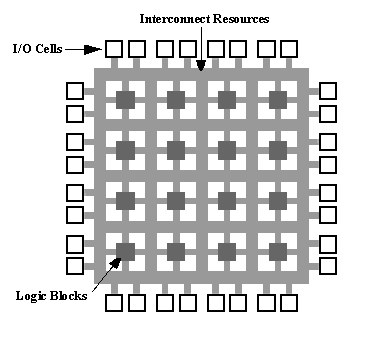
\includegraphics[width=0.5\textwidth,keepaspectratio=true]{./images/fpga1a}
 % \caption{Componentes de una FPGA}
  \label{fig:esquema}
 \end{center}
\end{figure}


%Conclusión!!Trabajar con un sistema final bajo licencias de hardware siguiendo el modelo de la Licencia LGPL para el software. Estamos comprometidos con el ideal de libre disposición, de libre uso y hardware de código abierto reutilizable.


 % OpenSource y Libre
\end{part}
\begin{part}{Estudio del Problema}
\newpage
%%%%%%%%%%%ESTUDIO DEL PROBLEMA%%%%%%%%%%%%%%%%
\chapter{Estudio del Problema}
	
	\section{Introducción}
	\par
	Como primera acción se analizó la factibilidad de implementación de un SoC con licencia OpenSource en FPGA, razón que condujo a la investigación del
	tópico en búsqueda de información necesaria que determine si existe tal posibilidad. Las características relevadas durante la investigación
	aportaron información respecto al hardware, las herramientas de desarrollo y el sistema operativo necesario para llevar a cabo la implementación. 
	\vspace{0.5cm}
	\par
	Para la selección del SoC se debió definir el microprocesador y los periféricos a utilizar, como así también las herramientas necesarias para la
	compilación y depuración de aplicaciones que corran sobre él. Esta situación derivó en una valoración de los diferentes entornos de desarrollo y
	sistemas operativos asociados que cumplan con el paradigma del software libre. Fue necesario además discernir entre las diversas alternativas de
	hardware que se tenían disponibles al momento del desarrollo de este trabajo compatibles con el SoC seleccionado. 
	\vspace{0.5cm}
	\par
	Fue necesario evaluar la posibilidad de implementar un Sistema Operativo que provea acceso mediante drivers a todos los periféricos conectados a
	la plataforma hardware elegida. La síntesis e implementación sobre FPGA requiere de aplicaciones específicas que debieron ponderarse para alcanzar el
	cumplimiento de los requerimientos.
	
	\newpage 
	
	\section{Requerimientos del Usuario}
	\par
	Se presenta en este apartado un listado de los requerimientos elecitados que tienen como objetivo comprender el dominio del problema y permiten
	trabajar en la realización de una solución eficiente.
	
		\subsection{En cuanto al Hardware}
		\begin{table}[h]
		\centering
		\begin{tabular}{ p{2.5cm} p{8cm} p{3cm} }
		\hline 
		\rowcolor[gray]{0.8} N\textordmasculine Req & Descripción & Tipo\\
		\hline
		RQX-HW 1 &  Se debe implementar un Microprocesador Softcore de núcleo simple & Cantidad y tipo de núcleos. \\
		\hline
		RQX-HW 2 &  El SoC seleccionado debe poseer la menor cantidad de restricciones respecto de su implementación en placas de desarrollo de diversos
		fabricantes. & Portabilidad a nivel Hardware\\
		\hline
		RQX-HW 3 & La placa de desarrollo elegida debe poseer al menos 32 MB de memoria RAM disponible que permita al ejecución del kernel de linux. &
		Memoria Disponible\\
		\hline
		RQX-HW 4 & La placa de desarrollo elegida debe poseer al menos 8 MB de memoria flash disponible que permita guardar la configuración de la FPGA y un
		bootloader & Memoria Disponible\\
		\hline
		\end{tabular}
		\caption{Listado de requerimientos de usuario - Hardware}
		\label{tab:requsr1}
		\end{table}
					
		\subsection{En cuanto a las Licencias}
		\begin{table}[h]
		\centering
		\begin{tabular}{ p{2.5cm} p{8cm} p{3cm} }
		\hline 
		\rowcolor[gray]{0.8} N\textordmasculine Req & Descripción  & Tipo\\
		\hline 
		RQX-LC 1 &  Todo el hardware implementado debe tener licencia LGPL o GPLv2 en su defecto & Licencias de hardware\\
		\hline 
		RQX-LC 2 &  Las herramientas de desarrollo utilizadas deben poseer licencias LGPL o GPLv2 en su defecto & Licencias de Software\\
		\hline
		RQX-LC 3 & El sistema operativo elegido debe poseer licencia LGPL o GPLv2 & Licencias de Software\\
		\hline
		\end{tabular}
		\caption{Listado de requerimientos de usuario - Licencias}
		\label{tab:requsr2}
		\end{table}
			
		\subsection{En cuanto a las Herramientas de Desarrollo}
		\begin{table}[h]
		\centering
		\begin{tabular}{ p{2.5cm} p{8cm} p{3cm} }
		\hline 
		\rowcolor[gray]{0.8} N\textordmasculine Req & Descripción  & Tipo\\
		\hline 
		RQX-HD 1 &  Las herramientas de desarrollo elegidas en base a la arquitectura a implementar deben tener la menor cantidad de restricciones respecto
		del sistema operativo donde serán ejecutadas & Portabilidad\\
		\hline 
		RQX-HD 2 &  Las herramientas de desarrollo deben brindar la capacidad de desarrollar y depurar programas para la arquitectura seleccionada &
		XXXXXXXXXXXX\\ % Revisar tipo de requerimiento
		\hline
		RQX-HD 3 &  Las herramientas de desarrollo de la placa seleccionada deben proveer soporte para el acceso a sus periféricos on board &
		XXXXXXXXXXXX\\ % Revisar tipo de requerimiento
		\hline 
		\end{tabular}
		\caption{Listado de requerimientos de usuario - Herramientas de Desarrollo}
		\label{tab:requsr3}
		\end{table}
		
		\subsection{En cuanto Sistema Operativo} 	 
		\begin{table}[h]
		\centering
		\begin{tabular}{ p{2.5cm} p{8cm} p{3cm} }
		\hline 
		\rowcolor[gray]{0.8} N\textordmasculine Req & Descripción  & Tipo\\
		\hline 
		RQX-SO 1 &  El sistema operativo elegido debe disponer de drivers y librerías que permitan el acceso a todos los dispositivos incluídos en el SoC &
		XXXXXXXXXXXXX\\ % Revisar tipo de requerimiento
		\hline 
		RQX-SO 2 &  El sistema operativo elegido debe tener la capacidad de ejecución multitarea e hilos & XXXXXXXXXXXX\\ % Revisar tipo de
		% requerimiento
		\hline
		RQX-SO 3 &  El sistema operativo elegido debe posibilitar la ejecución de aplicaciones de tiempo real & XXXXXXXXXXXX\\ % Revisar tipo de
		% requerimiento
		\hline 
		\end{tabular}
		\caption{Listado de requerimientos de usuario - Sistema Operativo}
		\label{tab:requsr4}
		\end{table}
	
	\section{Análisis de Riesgo}
		\subsection{Introducción}
        Para lograr producir aquello que se requiere, en el plazo solicitado y ajustados al presupuesto asignado, se necesita desarrollar
        un proceso que incluya desde la etapa más temprana la gestión de los riesgos asociados a los requerimientos, de forma que se contribuya al
        mejoramiento gradual del proceso de desarrollo y la gestión de un proyecto.
		\vspace{0.5cm}
		\par
        La gestión de riesgos procura formalizar conocimiento orientado a la minimización de riesgos en proyectos, mediante la
        generación de principios y buenas prácticas de aplicación realista \cite{etiqueta_riegos1}. Hasta el momento se ha propuesto
        y utilizado diferentes enfoques de gestión del riesgo desde que Boehm \cite{etiqueta_riegos2} atrajo a la comunidad de ingeniería del
        software hacia la gestión del riesgo. Sin embargo, es evidente que pocas organizaciones utilizan todavía de una forma explícita y sistemática
        métodos específicos para gestionar los riesgos en sus proyectos.
		\vspace{0.5cm}
		\par
        En \cite{etiqueta_riegos3} se presenta la definición de riesgo que plantea que el riesgo afecta a los futuros acontecimientos, implica
        cambios, e implica elección conjunto a la incertidumbre asociada a la misma. Es indiscutible que están presentes permanentemente las características de
        incertidumbre (acontecimiento que caracteriza al riesgo y que puede o no ocurrir) y de pérdida (si el riesgo se convierte en una realidad
        ocurrirán consecuencias no deseables o pérdidas).
		\vspace{0.5cm}
		\par
		Están definidas las categorías de riesgos: los riesgos del proyecto, que amenazan el plan; los riesgos técnicos, que amenazan la calidad y la
		planificación temporal; y los riesgos del negocio, que amenazan la viabilidad del proyecto o del producto. Otra categorización a considerar a
		partir del conocimiento que se tenga de ellos: los riesgos conocidos (los que se descubren en las evaluaciones); los riesgos predecibles (se
		extrapolan de la experiencia) y los riesgos impredecibles (pueden ocurrir, pero es muy difícil identificarlos de antemano).
		\vspace{0.5cm}
		\par
     	También son claras las estrategias frente al riesgo. Por un lado están las reactivas, cuyo método es evaluar las consecuencias del riesgo cuando
 		este ya se ha producido (ya no es un riesgo) y actuar en consecuencia. Este tipo de estrategias acarrea consecuencias negativas, al poner el
 		proyecto en peligro. Y por el otro las proactivas, que aplican el método de evaluación previa y sistemática de los riesgos y sus posibles
 		consecuencias, a la par que conforman planes de contingencias para de evitar y minimizar las consecuencias. Consecuentemente, este tipo de
 		estrategias permite lograr un menor tiempo de reacción ante la aparición de riesgos impredecibles.
		\vspace{0.5cm}
		\par
		De acuerdo con \cite{etiqueta_riegos3}, la administración o gestión de riesgos es un proceso iterativo que se aplica durante todo el proyecto y se
		desarrolla en cuatro etapas detalladas en la Figura ~\ref{fig:riesgos}. Se utilizó este modelo como guía para el análisis de los riegos del
		proyecto.
		
		\begin{figure}[!h]
 		\begin{center}
  		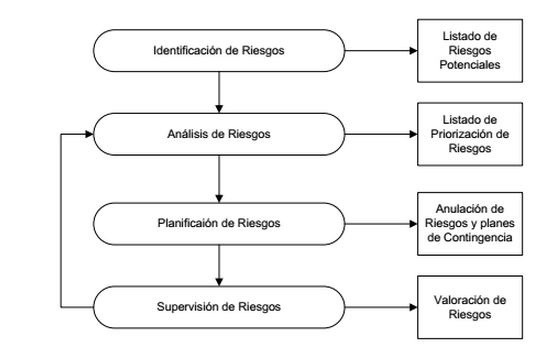
\includegraphics[width=0.8\textwidth,keepaspectratio=true]{./images/riesgos}
  		\caption{Procedimiento para la gestión de riesgos}
  		\label{fig:riesgos}
 		\end{center}
		\end{figure}
		
		\subsection{Identificación y análisis de riesgos}
		\par
		Se realizó un relevamiento inicial de riegos respecto de cada requerimiento de usuario planteado. Fue efectuado un análisis de severidad y
		probabilidad de ocurrencia para cada riesgo asociado. La severidad	del	impacto	de un riesgo concretado	se medió de la siguiente
		manera:
		
		\begin{itemize}
		  \item Catastrófico
		  \item Crítico	
		  \item Severo	
		  \item Menor	
		  \item Despreciable 
		\end{itemize}
	
		La probabilidad de ocurrencia se midió en base a la siguiente categorización:
	
		\begin{itemize}
		  \item Muy Probable
		  \item Probable	
		  \item Ocasional
		  \item Improbable 	
		  \item Remoto
		\end{itemize}
		
		En la Tabla ~\ref {tab:riegos} se listan los riesgos asociados, su severidad y probabilidad de ocurrencia para cada uno de los
		requerimientos de usuario.
		
		\begin{table}[!h]
		\centering
		\begin{tabular}{ p{2.5cm} p{9cm} p{2cm} p{2cm} }
		\hline 
		\rowcolor[gray]{0.8} N\textordmasculine Req & Riegos Asociados & Severidad  & Ocurrencia \\
		\hline
		RQX-HW 1& Código RTL con fallas reconocidas durante el proceso de síntesis & Crítica       & Probable \\
		\hline
				& Capacidad insuficiente para implementar la lógica del proyecto   & Catastrófico  & Ocasional\\	 
		\hline
		RQX-HW 2& Imposibilidad de acceso a alguno de los periféricos de la placa de desarrollo &  Crítica  & Probable\\
		\hline
		RQX-HW 3& Limitaciones de memoria RAM en las placas de desarrollo disponibles 	& Crítico  &  Improbable\\	 
		\hline
		RQX-HW 4& Limitaciones de memoria FLASH en las placas de desarrollo disponibles & Severo  &  Improbable\\ 
		\hline
		RQX-LC 1& Inexistencia de los Cores Open Source necesarios  	& Catastrófico  &  Ocasional\\
		\hline
				& Falta de documentación de apoyo para la implentación de los Cores  & Severo  &  Muy Probable\\ 
		\hline
		 		& Código RTL con fallas reconocidas durante el proceso de síntesis   & Critica & Probable\\ 
		\hline
		RQX-LC 2& Inexistencia de herramientas de desarrollo de hardware con licencias Open Source & Severo  &  Probable\\
		\hline
		RQX-LC 3& Inexistencia de herramientas de desarrollo de software con licencias Open Source & Severo  &  Improbable\\
		\hline
		RQX-LC 4& Inexistencia de un sistema operativo embebido con licencia Open Source  & Critico  &  Improbable\\
		\hline
		 		& Inexistencia de herramientas y librerias de sistema necesarias          & Critico  &  Probable\\
		\hline
		RQX-HD 1& Falta de herramientas de desarrollo portables a diversos sistemas operativos & Severo  &  Ocasional\\
		\hline		
		RQX-HD 2& Compilación cruzada incompatible con la arquitectura destino  & Critico &  Ocasional\\
		\hline
				& Falta de mecanismos de optimización de código del compilador  & Severo  &  Probable\\
		\hline
				& Imposibilidad de depuración de programas & Crítico  &  Probable\\
		\hline
		RQX-HD 3& Soporte de acceso a periféricos inexistente o con presencia de bugs & Critico &  Probable\\
		\hline
		RQX-SO 1& Drivers necesarios inexistentes o con fallos & Critico &  Probable\\
		\hline
				& Librerías necesarias inexistentes o con fallos & Severo &  Probable\\
		\hline
		RQX-SO 2& Incapacidad de ejección de hilos de los SO compatibles con el microprocesador elegido & Catastróficos & Improbable\\
		\hline
		RQX-SO 3& Limitaciones para la ejecución de SO de tiempo real & Critico & Probable\\
		\hline
		\end{tabular}
		\caption{Tabla de Riegos vs. Requerimientos}
		\label{tab:riegos}
		\end{table}
		
	\newpage	
			
	\section{Estudio de componentes}
		
			\subsection{Objetivo}
			Se estudiaron los componentes del proyecto y sus diversas alternativas de implementación por medio de un análisis comparativo que permitió evidenciar
			las características relevantes de cada uno de ellas. Inicialmente se realizó una comparativa de las prestaciones de los microprocesadores softcore
			más importantes para evaluar su capacidad de procesamiento. 
			
			\subsection{Selección del Microprocesador Soft-Core}
		
				\subsubsection{Comparación de Microprocesadores Soft-Core} 
	
				\subsubsection{Conclusiones de la elección del micro Soft-Core}
					 			
 			\subsection{Selección del SoC}
				\subsubsection{Comparación de proyectos SoC con procesador OpenRisc} 
				
				\paragraph{Proyecto MinSoC}
				La implementación llamada Minimal OpenRISC System on Chip utiliza IP cores estándar disponibles en OpenCores. Agrupa los cores necesarios para un
				SoC utilizando el procesador softcore OpenRISC OR1200. Este SoC puede ser sintetizado para cualquier FPGA y placa de desarrollo sin necesidad de
				realizar cambios en su descripción RTL. Para cumplir con esta premisa el proyecto se basa en una implementación básica de memoria y posee una
				unidad de debug llamada Advanced Debug System, que permite depurar el sistema y cargar los programas a ejecutar con la misma interfase utilizada
				para la configuración de la FPGA.
				
				El proyecto brinda soporte nativo a diversas placas y FPGAs mediante definiciones en el código RTL y archivos de constantes (constraint files)
				pero puede adaptarse a otras siguiendo una mínima serie de pasos. Se cuenta además con una serie testbenchs y firmwares que permiten realizar
				pruebas funcionales del sistema y son sirven de guía en los primeros desarrollos. Los testbenchs de MinSoC pueden ser ejecutados mediante la
				aplicación Icarus Verilog v.9.1. disponible en los repositorios estándar de la mayoría de las distribuciones Linux. 
				
				Existe una instancia de memoria on-chip de tamaño adaptable necesaria para soportar el firmware del CPU que conjuntamente con los cores que
				soportan los periféricos básicos son adaptados de acuerdo a las capacidades de la FPGA destino. 
				
				\paragraph{Proyecto ORPSoC}
				ORPSoC is the OpenRISC Reference Platform System-on-Chip. It is intended to be a development and verification environment for IP cores and SoC
				designs. It is a collaboratively developed project.
                As a development platform it should provide a modular, easy to use environment to perform RTL development with push-button simulation
                and synthesis flows. A basic software build environment is also present to support OpenRISC development in simulation and on target.
                The project should be easy enough for users, both new and experienced, to get started with OpenRISC designs and develop quickly and
                collaborate easily.
				
				
				
				\subsubsection{Conclusiones de la elección del micro Soft-Core}
 			
 			
 			\subsection{Selección de la Placa de Desarrollo}
 				\subsubsection{Análisis de las alternativas} 
				Los proyectos MinSoC y OrpSoc cuentan actualmente con soporte para diversas placas de desarrollo. 
				\paragraph{Xilinx}
				La empresa Xilinx provee kits de desarrollo de diversas características y prestaciones. A continuación se detallan algunas de las alternativas que
				son soportadas por los SoC elegidos.
				\subparagraph{S3ADSP1800A}
				El dispositivo XtremeDSP™ Starter Platform cuenta con una FPGA de la familia Spartan®-3A que permite la evaluación diseños para diferentes
				aplicaciones tales como Prototipado General, Sistemas Embebidos, Video Digital, DSP, Procesamiento de Imagenes, Comunicaciones digitales y
				Coprocesamiento. Esta plataforma provee acceso a las capacidades de la familia de FPGA Spartan®-3A y cuenta con periféricos,conectores e
				interfaces estándar de la industria. Fue diseñada para para ser utilizada con Xilinx System Generator para aplicaciones DSP y las herramientas de
				diseño ISE® o el entorno desarrollado en Linux llamado PetaLinux Software Development Kit (SDK) ambas herramientas provistas por el fabricante. 
				
				%Traducir esto ???
				Las características generales del kit son:
				
				\begin{tabular}{ p{4cm} p{10cm} }
				\rowcolor[gray]{0.8} Caracteristica & Descripción \\		
				\hline FPGA   & XC3SD1800A-4FGG676C Spartan-3A DSP FPGA\\
				\hline Clocks & 125 MHz LVTTL SMT oscillator\\
				\hline        & LVTTL oscillator socket\\
				\hline		  & 25.175 MHz LVTTL SMT oscillator (video clock)\\
				\hline		  & 25 MHz Ethernet clock (accessible to FPGA)\\
				\hline Memory & 128 MB (32M x 32) DDR2 SDRAM\\
				\hline		  & 16Mx8 parallel / BPI configuration flash\\
				\hline 		  & 64 Mb SPI configuration / storage flash (with 4 extra SPI selects)\\
				\hline Interfaces & 10/100/1000 PHY\\
				\hline			  & JTAG programming/configuration port\\
				\hline            & RS232 Port\\
				\hline			  & Low-cost VGA\\
				\hline			  & 4 SPI select lines\\
				\hline Buttons and Switches & 8 user LEDs\\
				\hline  		  & 8-position user DIP switch\\
				\hline            & 4 user push button switches\\
				\hline 			  & Reset push button switch\\
				\hline User I/O and Expansion & Digilent 6-pin header\\
				\hline			 			  & EXP expansion connector\\
				\hline 						  & 30-pin GPIO connector: can be used for System ACE™ Compact Flash daughter card (not included)\\
				\hline Configuration and Debug & JTAG\\
				\hline                         & System ACE module connector\\   
				\end{tabular}
				
				Las implementaciones MinSoC y ORPSoC proveen soporte nativo para los siguientes periféricos:
				
				\begin{itemize}
				  \item Ethernet
				  \item GPIO (Solo ORPSoC)
				  \item DDR2 SDRAM (128MB) (Solo ORPSoC)
				  \item SPI
				  \item UART				
				\end{itemize}
			
				\subparagraph{ML501}
				La ML501 es una plataforma de desarrollo de bajo costo y gran funcionalidad que provee un acceso práctico a los recursos disponibles en el
				dispositivo FPGA Virtex®-5 LX50. Posee interfases y conectores industriales estándar y presenta gran versatilidad para su utilización en
				múltiples aplicaciones como Video, Audio y puertos de comunicación.
				
				Las características generales del kit son:
			
			\begin{tabular}{ p{4cm} p{10cm} }
			\rowcolor[gray]{0.8} Caracteristica & Descripción \\		
			\hline FPGA & XC5VLX50FFG676\\
			\hline Memoria & DDR2 SODIMM (256 MB)\\
			\hline 		   & ZBT SRAM (1 MB)\\
			\hline 		   & Linear Flash (32 MB)\\
			\hline         & System ACE™ CF technology (Compact Flash)\\
			\hline         & Platform Flash\\
			\hline         & SPI Flash\\
			\hline Clocks  & External clocking (2 differential pairs)\\
			\hline Interfaces & USB (2) - host and peripheral\\
			\hline 			  & PS/2 (2) - keyboard, mouse\\
			\hline 			  & RJ-45 - 10/100 Networking\\
			\hline 			  & RS-232 (male) - serial port\\
			\hline 			  & Audio In (2) - line, microphone\\
			\hline 			  & Audio Out (2) - line, amp, SPDIF, piezo speaker\\
			\hline 			  & Video (DVI/VGA) Output\\
			\hline I/O y expansión & Single-ended and differential I/O expansion\\
			\hline GPIO		&  DIP switch (8)\\
			\hline 			&  LEDs (8)\\
			\hline 			&  push buttons (5)\\
			\hline Debug y programación & JTAG programming interface\\
			\hline Medioambiente & EU-RoHS compliant \\
			\end{tabular}
				
				Las implementación ORPSoC fue probada con éxito en esta plataforma y provee soporte para los siguientes periféricos:
				
				\begin{itemize}
				  \item Ethernet
				  \item GPIO
				  \item DDR2 SDRAM (256MB)
				  \item CFI flash (32MB)
				  \item SRAM
				  \item SPI
				  \item UART
				  \item AC97 
				  \item PS/2 				
				\end{itemize}
			
				
				\paragraph{Digilent}
				\subparagraph{Atlys}
				La placa de desarrollo Atlys es una plataforma que permite el desarrollo de circuitos digitales y esta soportada por una FPGA Xilinx Spartan 6
				LX45. Posee periféricos entre los que se destacan Gbit Ethernet, Video HDMI, Audio, puertos USB y Memoria Ram 128 MB DDR2 que permiten el
				desarrollo de Sistemas Digitales sobre procesadores embebidos como  MicroBlaze de Xilinx. Atlys es compatible con todas las herramientas CAD de
				Xilinx como ChipScope, EDK y WebPack (gratuito) lo que permite completar diseños sin mayor costo. Como alternativa puede utilizarse un entorno de
				desarrollo para Linux llamado PetaLinux Software Development Kit (SDK) provisto por el fabricante de la FPGA.
				
				Las características generales de la plataforma son:
				
				\begin{tabular}{ p{4cm} p{10cm} }
				\rowcolor[gray]{0.8} Caracteristica & Descripción \\		
				\hline FPGA   & Spartan-6 LX45, 324-pin BGA package \\
				\hline 		  &	6,822 slices each containing four 6-input LUTs and eight flip-flops\\
				\hline DSP	  & 58 DSP slices\\
				\hline Clocks & 2.1Mbits of fast block RAM\\
				\hline 		  & 4 clock tiles (8 DCMs \& 4 PLLs)\\
				\hline 		  & 6 phased-locked loops\\
				\hline 		  & 500MHz+ clock speeds\\
				\hline 		  & 100MHz CMOS oscillator\\
				\hline Memoria & 128Mbyte DDR2 16-bit wide data\\
				\hline         & 16Mbyte x4 SPI Flash for configuration \& data storage\\
				\hline GPIO & 8 LEDs \\
				\hline 		& 6 buttons\\
				\hline		& 8 slide switches\\
				\hline Interfaces & 10/100/1000 Ethernet PHY\\
				\hline 			  & On-board USB2 ports for programming \& data transfer\\
				\hline 			  & USB-UART and USB-HID port (for mouse/keyboard)\\
				\hline 			  & Two HDMI video input ports \& two HDMI output ports\\
				\hline			  & AC-97 Codec with line-in, line-out, mic, \& headphone\\
				\hline Energía & Real time power monitors on all power rails\\
				\hline 		   & 20W power supply and USB cable\\
				\hline I/O y Expansión & 48 I/O’s routed to expansion connectors\\
				\end{tabular}
				
				La implementación ORPSoC proveen soporte nativo para los siguientes periféricos:
				
				\begin{itemize}
				  \item AC97
				  \item Ethernet
				  \item GPIO
				  \item PS/2 
				  \item DDR2 SDRAM (128MB)
				  \item SPI
				  \item UART
				  \item VGA
				\end{itemize}				

				\paragraph{Terasic}
				\subparagraph{Terasic DE0 Nano}
				La plataforma DE0-Nano posee un tamaño compacto que se ajusta al diseño de circuitos para proyectos portables. Fue diseñada para ser
				utilizada con una implementación simple utilizando como destino una FPGA Cyclone IV de Altera con 22,320 LEs (Elementos Lógicos). Entre sus
				características princpiales se encuentran diversas interfases que incluyen dos puertos de expanxión GPIO, dispositivos de memoria on board SDRAM y
				EEPROM. Las mayores ventajas del DE0-Nano son su reducido tamaño y peso, así como la capacidad de ser reconfigurado sin la necesidad de
				utilización de hardware extra. Los requerimientos de energía para dispositivos portables son cruciales , la DE-0 Nano posee 3 esquemas posibles
				de conexión : un puerto USB mini-AB, conectores de 2 pines para alimentación externa de 5V, y 2 pines de 5V.

				Las características generales de la plataforma son:
				
				\begin{tabular}{ p{4cm} p{10cm} }
				\rowcolor[gray]{0.8} Caracteristica & Descripción \\		
				\hline FPGA   	& Cyclone® IV EP4CE22F17C6N FPGA\\
				\hline 			& 22,320 Logic elements (LEs)\\
				\hline 			& 594 Embedded memory (Kbits)\\
				\hline 			& 66 Embedded 18 x 18 multipliers\\
				\hline			& 4 General-purpose PLLs\\
				\hline 			& 153 Maximum FPGA I/O pins\\ 
				\hline Configuration Status and Set-Up Elements & 	On-board USB-Blaster circuit for programming\\
				\hline											&	FPGA Serial Configuration Device (EPCS)\\
				\hline Expansion Header & 	Two 40-pin Headers (GPIOs) provides 72 I/O pins\\
				\hline 					&	Two 5V power pins, two 3.3V power pins and four ground pins\\
				\hline 					&	One 26-pin header provides 16 digital I/O pins and 8 analog input pins to connect to analog sensors, etc\\ 
				\hline Memory Devices	&	32MB SDRAM\\
				\hline 					&	2Kb I2C EEPROM\\ 
				\hline General User Input/Output 	& 8 green LEDs\\
				\hline 								& 2 debounced push-buttons\\
				\hline 								& 4 dip switches\\ 
				\hline G-Sensor & ADI ADXL345, 3-axis accelerometer with high resolution (13-bit)\\ 
				\hline A/D Converter & NS ADC128S022, 8-Channel, 12-bit A/D Converter\\ 
				\hline					 & 50 ksps to 200 ksps \\
				\hline Clock System & On-board 50MHz clock oscillator\\
				\hline Power Supply & USB Type mini-AB port (5V)\\
				\hline 				& Two DC 5V pins of the GPIO headers (5V)\\
				\hline 				& 2-pin external power header (3.6-5.7V)\\
				\end{tabular}
				
				La implementación ORPSoC proveen soporte nativo para los siguientes periféricos:
				
				\begin{itemize}
				  	\item GPIO
					\item SDRAM (32MB)
					\item UART
					\item SPI FLASH (8MB)
					\item I2C
				\end{itemize}				
				
 				\subsubsection{Conclusiones de la elección de la Placa de Desarrollo}
 				Se seleccionó entre los items analizados y teniendo en cuenta la disponibilidad de recursos al momento de realizar este trabajo utilizar las
 				placas S3ADSP1800A de Xilinx para soportar los SoC a implementar.
 			
 			\subsection{Selección de las herramientas de desarrollo} 	 
 		
 		
 			\subsection{Selección del Sistema Operativo}
 			 % Estudio del Problema
\newpage

\chapter{Descripción microprocesadores disponibles en el mercado}
	\section{Soft-Core Processors}
	Un soft-core processor o abreviado SCP, también llamado soft microprocessor o soft  processor, es un microprocesador que puede ser implementado
	utilizando síntesis lógica en  diferentes dispositivos lógicos programables como CPLDs o FPGAs, o incluso puede ser incluido en un diseño para ASIC.
 	Suelen ser distribuidos en forma de código fuente en algún lenguaje de descripción de hardware, principalmente VHDL o Verilog, aunque  algunos SCPs
 	comerciales se distribuyen en formatos propietarios.
	Los principales fabricantes de dispositivos lógicos programables como se dijo en capitulos anteriores tienen su propio  SCP comercial especialmente
	diseñado y optimizado para funcionar en sus propias FPGAs. Así Xilinx tiene el PicoBlaze \cite{Etiqueta15} y el MicroBlaze \cite{Etiqueta16}, Altera
	proporciona el Nios II \cite{Etiqueta17}, y Lattice distribuye su LatticeMico32 \cite{Etiqueta18}. También existen una gran variedad de SCPs
	distribuidos en forma de código abierto, como el OpenRISC 1200 \cite{Etiqueta19} mantenido por la comunidad Opencores \cite{Etiqueta20}, o los  SCPs
	LEON2 y LEON3 \cite{Etiqueta21} \cite{Etiqueta22} que proporciona la compañía Gaisler Research \cite{Etiqueta23}.
		
	A continuación se presentan más detalladamente las características de estos SCPs, y un resumen comparativo de sus características
	\subsection{PicoBlaze}
	
	PicoBlaze es un microcontrolador RISC de 8 bits desarrollado por Xilinx y optimizado para sus FPGAs. Esta optimizado para ocupar muy poco área, tan sólo 96 slices, y en cuanto a velocidad puede llegar a ejecutar entre 44 y 100 millones de instrucciones por segundo, dependiendo del speedgrade y la familia de FPGA sobre la que se implemente. Las principales características del PicoBlaze son:
	
  
	\begin{itemize}
	  \item  16 Registros de propósito general de 1 byte.
	  \item 1024 bytes de instrucciones en memoria on-chip que se cargan al programarse la FPGA.
	  \item 256 puertos de entrada y 256 de salida para conectar lógica o periféricos externos.
	\end{itemize}
	
	La arquitectura general consiste en una serie de bloques presentados en la figura ~\ref{fig:PicoBlazer}.
		
	\begin{figure}[h!]
 	\begin{center}
  	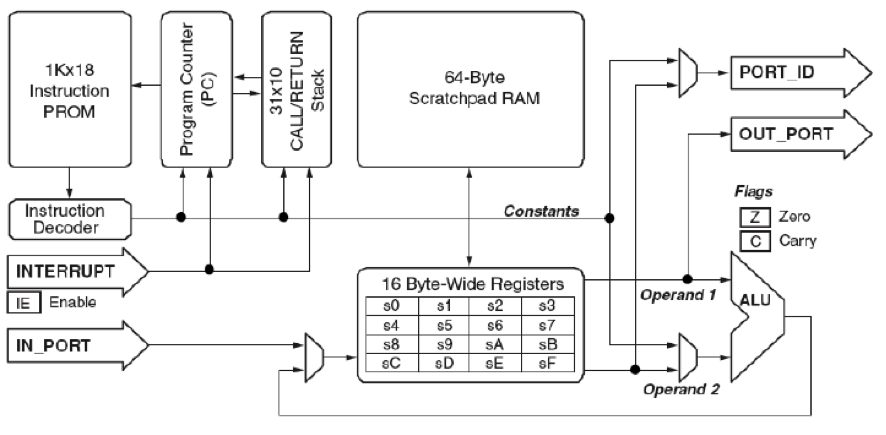
\includegraphics[width=0.8\textwidth,keepaspectratio=true]{./images/estructurapico}
  	\caption{estructura interna del microcontrolador PicoBlaze}
  	\label{fig:PicoBlazer}
 	\end{center}
	\end{figure}

Aunque está más orientado para ser usado en pequeñas tareas de control más que en ejecutar grandes aplicaciones, se ha usado ya en varios sistemas multiprocesador.

	\subsection{MicroBlaze}

MicroBlaze es un microprocesador RISC de 32 bits desarrollado por Xilinx para sus FPGAs de las familias Spartan y Virtex. Sigue una arquitectura Harvard con buses de memoria de datos e instrucciones separados. Una de sus principales características es que es muy configurable, pudiendo incluir o excluir una serie de elementos del microprocesador según las necesidades de la aplicación objetivo permitiendo una gran variedad de configuraciones más o menos rápidas y que ocupan más o menos área en la FPGA.

Las características más destacables de este SCP son:    

	\begin{itemize}
	  \item  32 registros de propósito general de 32 bits.
	  \item  Instrucciones de 32 bits, con 3 operandos y 2 modos de direccionamiento.
	  \item  Bus de direcciones de 32 bits.
	  \item  Pipeline configurable de 3 o 5 etapas.
	  \item  FPU,\textit{ barrel-shifter} y multiplicador y/o divisor de enteros opcionales.
	  \item  Caché de instrucciones y caché de datos opcionales.
	  \item  32 registros de propósito general de 32 bits.
	  \item   3 interfaces de bus disponibles para conectar distintos tipos de periféricos:
		\begin{itemize}
		  \item  LMB \cite{Etiqueta23}(\textit{Local Memory Bus}): Bus síncrono de alta velocidad utilizado principalmente para conectar los bloques de memoria interna de la FPGA.
	 	 \item  OPB \cite{Etiqueta24}(\textit{On-Chip Memory Bus}) : Bus síncrono utilizado para conectar periféricos con tiempos de acceso variables. Tiene soporte para hasta 8 maestros.
	 	 \item FSL\cite{Etiqueta25} (\textit{Fast Simplex Link}): Canales punto a punto dedicados, para streaming de datos. Dispone de 8 canales, cada uno con un puerto de entrada y otro de salida.
		\end{itemize}
	\end{itemize}

La arquitectura general consiste en una serie de bloques presentados en la figura ~\ref{fig:MicoBlazer}.
		
	\begin{figure}[h!]
 	\begin{center}
  	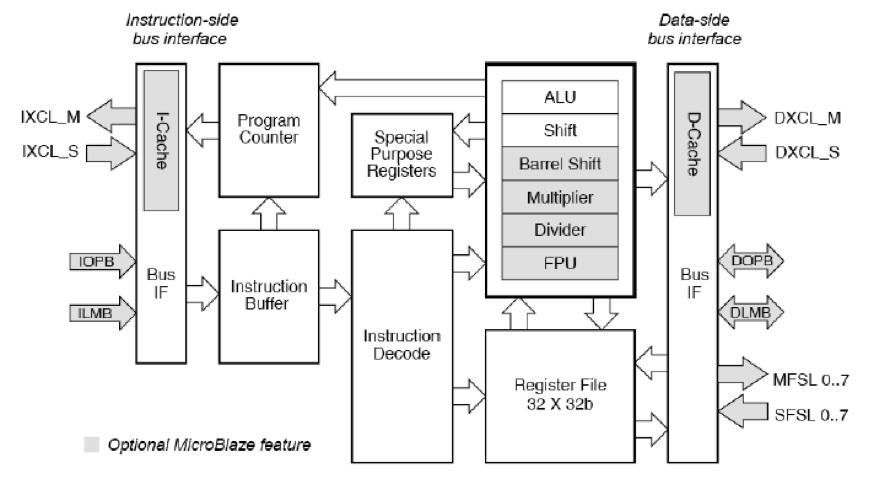
\includegraphics[width=0.8\textwidth,keepaspectratio=true]{./images/estructuramicroblazer}
  	\caption{estructura interna del microcontrolador MicoBlaze}
  	\label{fig:MicoBlazer}
 	\end{center}
	\end{figure}

Actualmente MicroBlaze es uno de los SCP más utilizado, y parte del éxito se debe
a las herramientas que proporciona Xilinx para crear sistemas basados en este
microprocesador. La herramienta Xilinx Platform Studio\cite{Etiqueta26}permite de forma gráfica e
intuitiva interconectar tanto el procesador como los distintos periféricos y buses que forman
el sistema
~\ref{fig:Xilinx Platform Studio}

\begin{figure}[h!]
 	\begin{center}
  	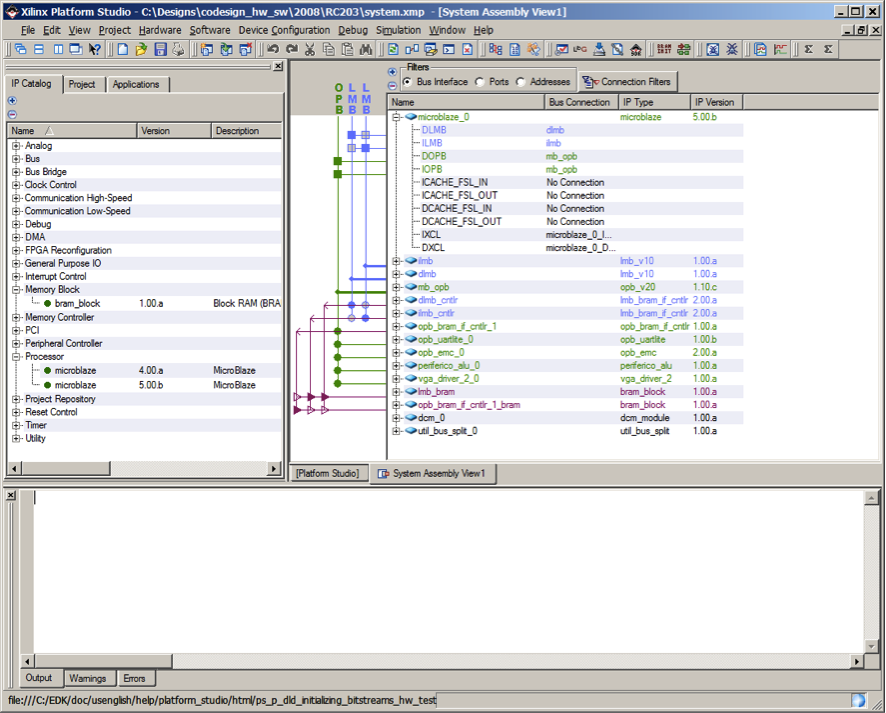
\includegraphics[width=0.8\textwidth,keepaspectratio=true]{./images/herramientaxps}
  	\caption{interfaz de la herramienta Xilinx Platform Studio}
  	\label{fig:Xilinx Platform Studio}
 	\end{center}
	\end{figure}

También ofrece una librería de IPs ya diseñadas y listas para integrarse en cualquier diseño como:

		\begin{itemize}
		  \item  Controladores de memoria: SRAM, SDRAM, DDR y DDR2.
	 	 \item  Dispositivos de comunicación serie: bus I2C, UART16550.
	 	 \item Controladores Ethernet y Ethernet Lite.
		\end{itemize}

La herramienta además de ayudar y simplificar la parte de diseño hardware de un sistema basado en el procesador MicroBlaze también ofrece facilidades para el desarrollo de software para el sistema, proporcionando tanto drivers para los distintos periféricos como todo un conjunto de herramientas de desarrollo software (compilador, depurador, bootloader, …), un micro kernel con interfaz de hilos POSIX y diversas librerías, todo ello integrado en un entorno basado en Eclipse\cite{Etiqueta27} que facilita mucho la tarea del programador de aplicaciones.

	\subsection{Nios II}

Nios II es el procesador que ofrece la compañía Altera para ser usado en sus FPGAs de las familias Stratix y Ciclone. Es un procesador RISC de 32 bits con arquitectura Harvard.

 Las principales características de este SCP son:

		\begin{itemize}
		  \item  32 registros de propósito general de 32 bits.
	 	 \item  Operaciones de punto flotante de precisión simple.
	 	 \item  Bus de direcciones de 32 bits.
		 \item  Posibilidad de añadir lógica a la ALU para crear nuevas instrucciones de propósito específico.
 		\item Caché de instrucciones y caché de datos opcionales.
		\end{itemize}
  
Altera ofrece tres versiones diferentes del Nios II, con diferentes características en cuanto a rendimiento y consumo de área.

 Las principales características de cada versión del procesador son:
   
		\begin{itemize}
		  \item Nios II \textit{fast}: diseñado para ser lo más rápido posible, cuenta con un pipeline de 6 etapas. Incluye operación de multiplicación por hardware en un solo ciclo, previsión dinámica de saltos y cachés separadas de instrucciones y datos.
	 	 \item Nios II \textit{economy}: diseñado para ocupar la menor área posible, ocupa tan solo 700 Logic Elements. Sin caches.
 		\item Nios II \textit{standard}: orientado a aplicaciones de bajo coste, con un rendimiento medio en las aplicaciones. Incluye caché de instrucciones, pipeline de 5 etapas y predicción estática de saltos. También ofrece multiplicador, divisor y desplazador hardware opcionales.
		\end{itemize}

\begin{figure}[h!]
 	\begin{center}
  	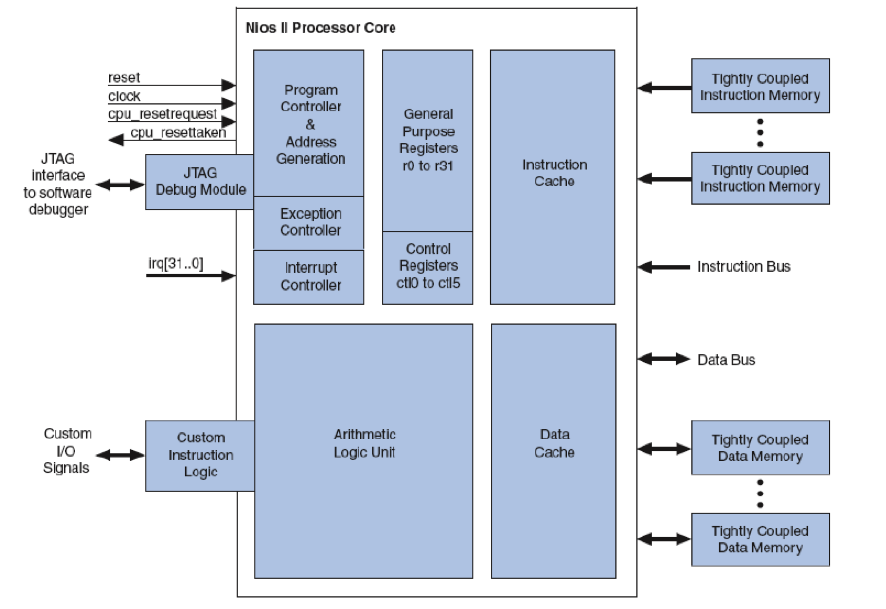
\includegraphics[width=0.8\textwidth,keepaspectratio=true]{./images/nios2}
  	\caption{arquitectura del procesador Nios II}
  	%\label{fig:Xilinx Platform Studio}
 	\end{center}
	\end{figure}

Al igual que Xilinx, Altera también ofrece una herramienta gráfica que permite crear de forma rápida y sencilla sistemas basados en su microprocesador: System on Programmable Chip Builder \cite{Etiqueta28}~\ref{fig:System on Programmable Chip Builder}. También ofrece una librería de componentes como UARTs, dispositivos Ethernet, controladores de memoria, etc, que se pueden integrar a cualquier diseño basado en Nios II.
Además de facilitar la tarea de diseñar la parte hardware del sistema, también ofrece un entorno de desarrollo de software basado en Eclipse que facilita la tarea del desarrollador de software proporcionándole en un único IDE todas las herramientas necesarias como editor, compilador, depurador, bootloader, etc, además de dar soporte para desarrollar aplicaciones que hagan uso del sistema operativo MicroC/OS-II.

	\begin{figure}[h!]
 	\begin{center}
  	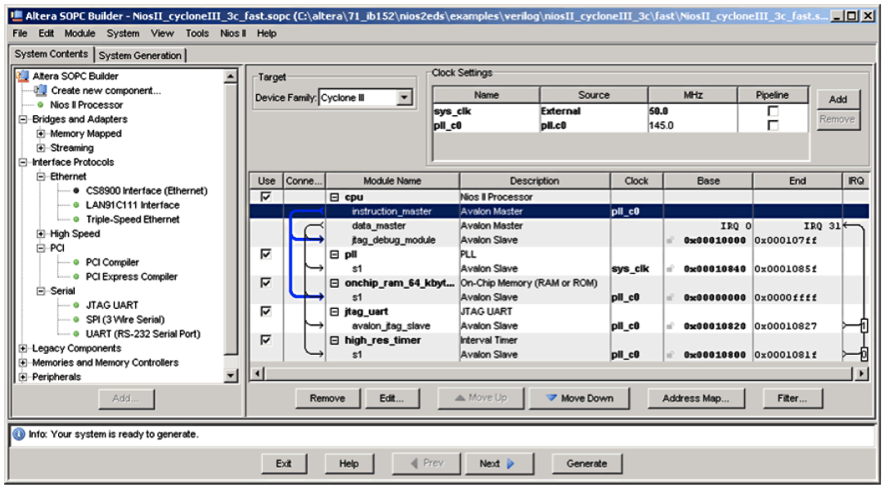
\includegraphics[width=0.8\textwidth,keepaspectratio=true]{./images/herramientasnios2}
  	\caption{interfaz de la herramienta System on Programmable Chip Builder}
  	\label{fig:System on Programmable Chip Builder}
 	\end{center}
	\end{figure}

	\subsection{LatticeMico32}
 
La compañía Lattice ofrece el procesador LatticeMico32 para usarlo en sus FPGAs. Una de las principales características de este procesador es que aunque proviene de una compañía privada se ofrece bajo una licencia libre. Sigue una arquitectura RISC, y utiliza dos interfaces de bus WISHBONE \cite{Etiqueta34}separados para instrucciones y datos.

 El procesador se ofrece en 3 posibles configuraciones con distintas relaciones de área y rendimiento:

\begin{itemize}
		  \item Configuración básica: Sin multiplicador hardware ni cachés. Desplazador multiciclo. Ocupa 1571 LUTs de una FPGA LatticeEC/ECP y puede alcanzar una frecuencia de reloj de 81 MHz.
		 \item Configuración estándar: Con multiplicador hardware, desplazador segmentado y 8 KB de caché de instrucciones. Caché de instrucciones y caché de datos opcionales.Ocupa 2040 LUTS y alcanza una frecuencia de reloj de 89 MHz.
 		\item Completa: Igual que la configuración estándar pero con 8 KB de caché de datos. Ocupa 2230 LUTs y alcanza los 92 MHz.
		\end{itemize}

\begin{figure}[h!]
 	\begin{center}
  	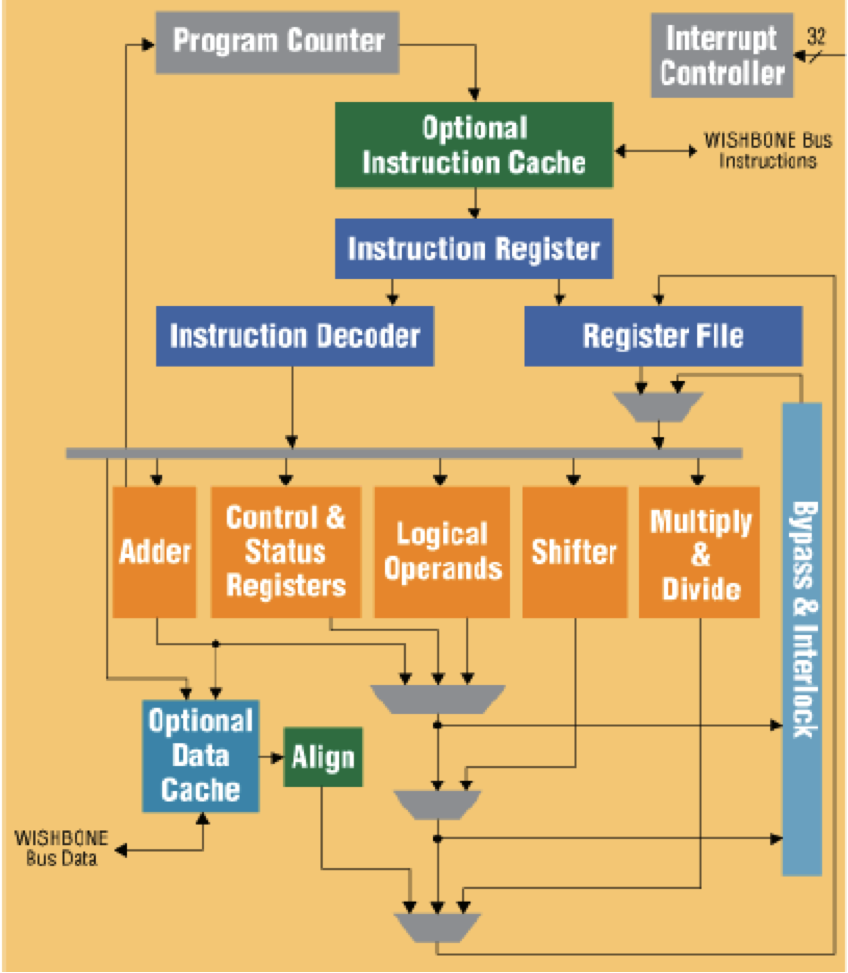
\includegraphics[width=0.5\textwidth,keepaspectratio=true]{./images/latice}
  	\caption{arquitectura del procesador LatticeMico32}
  	%\label{fig:System on Programmable Chip Builder}
 	\end{center}
	\end{figure}

Al igual que sus competidoras Xilinx y Altera, Lattice ofrece también un entorno de desarrollo para generar sistemas basados en su microprocesador
llamada Mico System Builder. Desde dicha herramienta permite de forma sencilla interconectar el procesador con los distintos periféricos y buses que
integra la librería de IPs proporcionada por Lattice.

\begin{figure}[h!]
 	\begin{center}
  	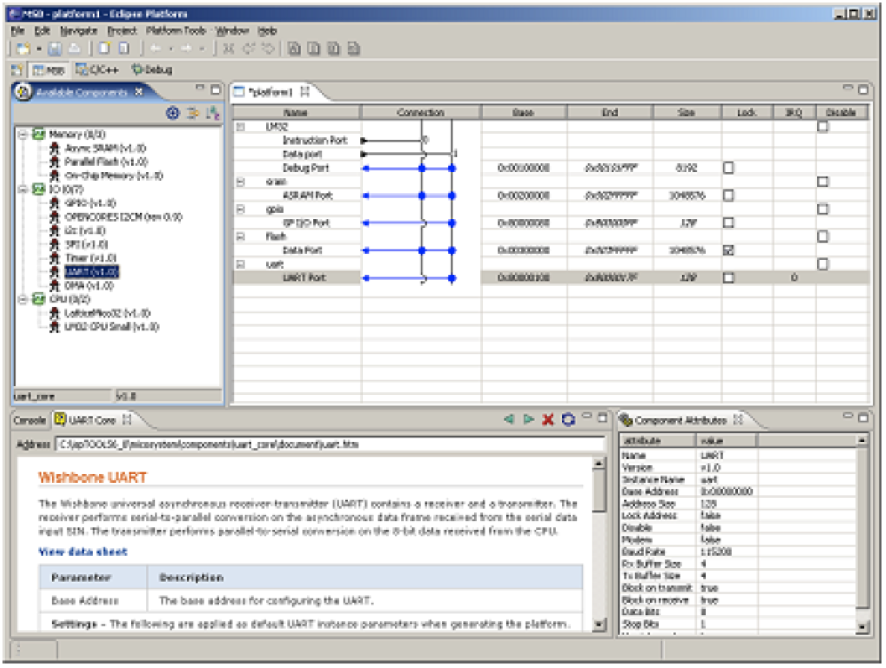
\includegraphics[width=0.8\textwidth,keepaspectratio=true]{./images/herramientaslatice}
  	\caption{interfaz de la herramienta Mico System Builder}
  	%\label{fig:System on Programmable Chip Builder}
 	\end{center}
	\end{figure}

	\subsection{OpenRISC 1200}

Opencores \cite{Etiqueta20} es una comunidad de hardware de código abierto que ofrece una gran variedad de IPs entre los que se encuentra su producto estrella: el OpenRISC 1200, un microprocesador RISC de 32 bits que se distribuye como código abierto.

Algunas características de este SCP son:

\begin{itemize}
		 \item  3Arquitectura Harvard.
	 	 \item \textit{Pipeline} de 5 etapas.
	 	 \item  Unidad de manejo de memoria (MMU)
		 \item  Cachés de instrucciones y de datos de 8 KB, de mapeo directo.
 		\item Unidades opcionales como: unidad de depuración,\textit{ tick-timer}, controlador de interrupciones y unidad de manejo de potencia (PMU).
		\item Interfaz WISHBONE para los buses de instrucciones y de datos.
\end{itemize}
  
\begin{figure}[h!]
 	\begin{center}
  	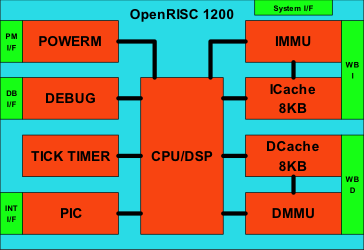
\includegraphics[width=0.6\textwidth,keepaspectratio=true]{./images/OR1200}
  	\caption{arquitectura OpenRISC}
  	%\label{fig:System on Programmable Chip Builder}
 	\end{center}
	\end{figure}


Las herramientas existentes para desarrollar sistemas basados en el OpenRISC 1200 son muy limitadas y no existe una herramienta similar a las existentes para los procesadores ya comentados que permita interconectar el procesador y los distintos buses y periféricos de una forma sencilla e intuitiva. Existe una herramienta gráfica basada en TCL/TK que permite configurar las diferentes características del procesador de forma sencilla\cite{Etiqueta29}, en lugar de tener que editar a mano el fichero de configuración del microprocesador.

En cuanto a herramientas para el desarrollo de software está también bastante limitado. Se proporcionan las herramientas de compilación y depuración de GNU, y existen también proyectos que mantienen ports de algunos sistemas operativos libres como eCos\cite{Etiqueta30} o uCLinux \cite{Etiqueta31}. Pero no está todo integrado en un entorno de desarrollo ni ofrece las características que ofrecen las herramientas de Xilinx o Altera como generación automática de drivers, generación de scripts de enlazado, generación de BSPs para distintos sistemas operativos, etc.

El rendimiento que ofrece el OpenRISC 1200 es superior al de sus competidores comerciales, a costa de un mayor consumo de área. En \cite{Etiqueta32} se ofrecen diversos datos de comparación de distintos procesadores en distintas configuraciones y se desprende que el área ocupada por un sistema basado en OpenRISC 1200 es entre dos y tres veces superior al de un sistema equivalente basado en MicroBlaze.

   	\subsection{LEON 2 y LEON 3}

LEON 2 es un procesador RISC de 32 bits basado en la arquitectura SPARC-V8\cite{Etiqueta33}. Está desarrollado por Gaisler Research y la Agencia Espacial Europea (ESA). Está completamente descrito en VHDL sintetizable y se distribuye bajo una licencia GPL (General Public License). Algunas de sus características más importantes son:

\begin{itemize}
		 \item  Arquitectura Harvard.
		 \item  Caches de instrucciones y datos configurables.
	       \item \textit{Pipeline} de 5 etapas.
		 \item  Interfaz de bus AMBA.
 		\item  Caché de datos con protocolo \textit{snoop}, que permite coherencia de cachés en sistemas multiprocesador.
		\item Unidad de manejo de memoria (MMU).
		\end{itemize}
	
\begin{figure}[h!]
 	\begin{center}
  	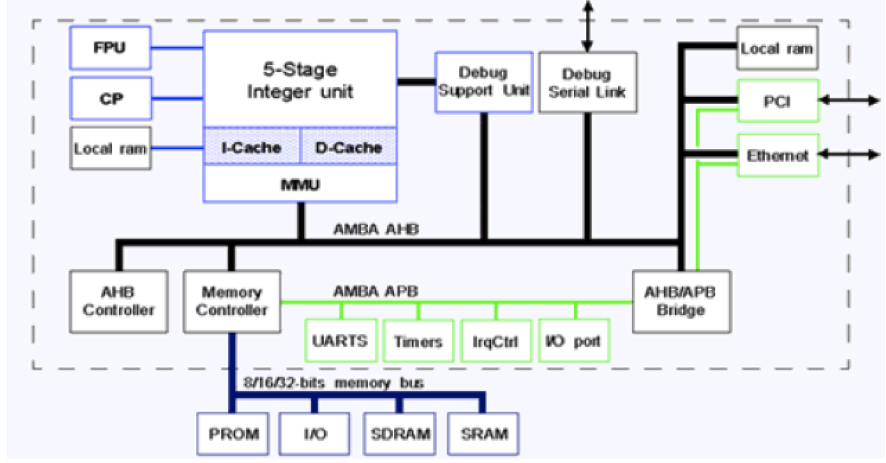
\includegraphics[width=0.8\textwidth,keepaspectratio=true]{./images/leon}
  	\caption{arquitectura del procesador LEON 2}
  	%\label{fig:System on Programmable Chip Builder}
 	\end{center}
	\end{figure}

Existe una herramienta gráfica que permite configurar las partes opcionales del procesador, pero no existe ninguna herramienta que permita realizar de forma sencilla las conexiones entre buses y periféricos, añadir nuevos periféricos, etc que ofrecen las herramientas comerciales de otros procesadores. En la parte de desarrollo software Gaisler Research proporciona el compilador basado en gcc LECCS, y RTEMS un kernel de tiempo real para ser usado con su procesador. También existen ports de otros kernels como eCos o Linux, mantenidos por terceras partes.

En cuanto a rendimiento el LEON 2 es muy superior a todos los procesadores presentados hasta ahora, aunque también es el que ocupa más área: de los resultados que se presentan en \cite{Etiqueta32} se puede ver que en media ocupa entre 3 y 4 veces más que un sistema equivalente basado en MicroBlaze y entre 1 y 1,5 veces más que un sistema equivalente basado en OpenRISC 1200. 

El LEON 2 dejó de estar soportado y dio paso al LEON 3: un procesador RISC de 32 bits, también compatible con la arquitectura SPARC V8 y que incluye muchas mejoras con respecto a su predecesor:

\begin{itemize}
		 
	       \item \textit{Pipeline} de 7 etapas.
		 \item Unidad de punto flotante completamente segmentada.
		 \item Cachés de instrucciones y de datos mejoradas, hasta 4 veces más grandes.
 		\item  Caché de datos con protocolo \textit{snoop}, que permite coherencia de cachés en sistemas multiprocesador.
		\item Hasta un 50 \% más de frecuencia de reloj.
		\item Soporte para multiprocesamiento simétrico.
		\end{itemize}
   
Todas estas mejoras suponen también un considerable aumento del área necesaria, en torno a un 30 \% más.

 % Micros disponibles
\newpage
\chapter{Selección de Componentes}

\section{Objetivo}
			Se estudiaron los componentes del proyecto y sus diversas alternativas de implementación por medio de un análisis comparativo que permitió evidenciar
			las características relevantes de cada uno de ellas. Inicialmente se realizó una comparativa de las prestaciones de los microprocesadores softcore
			más importantes para evaluar su capacidad de procesamiento.

\section{Selección del Microprocesador Soft-Core}


En la elección de los microprocesadores Soft-Core presentados en el capitulo anterior nos basamos principalmente en el requerimiento de usuario sobre el Hardware el cual nos requería implementar un Microprocesador Soft-core el que prestara un rendimiento igual o superior a sus competidores comerciales. Tras la evaluación de las ventajas y desventajas de la elección de un micro con estas características se determinó el uso del microprocesador OpenRISC 1200. 	


		    
			


\section{Presentación de los SoC basados en OpenRISC}
				
				\subsection{Proyecto MinSoC}
				La implementación llamada Minimal OpenRISC System on Chip utiliza IP cores estándar disponibles en OpenCores. Agrupa los cores necesarios para un SoC utilizando el procesador softcore OpenRISC OR1200. Este SoC puede ser sintetizado para cualquier FPGA y placa de desarrollo sin necesidad de realizar cambios en su descripción RTL. Para cumplir con esta premisa el proyecto se basa en una implementación básica de memoria y posee una unidad de debug llamada Advanced Debug System, que permite depurar el sistema y cargar los programas a ejecutar con la misma interfase utilizada para la configuración de la FPGA.				El proyecto brinda soporte nativo a diversas placas y FPGAs mediante definiciones en el código RTL y archivos de constantes (constraint files)
				pero puede adaptarse a otras siguiendo una mínima serie de pasos. Se cuenta además con una serie testbenchs y firmwares que permiten realizar
				pruebas funcionales del sistema y sirven de guía en los primeros desarrollos. Los testbenchs de MinSoC pueden ser ejecutados mediante la
				aplicación Icarus Verilog v.9.1. disponible en los repositorios estándar de la mayoría de las distribuciones Linux. 
				
				Existe una instancia de memoria on-chip de tamaño adaptable necesaria para soportar el firmware del CPU que conjuntamente con los cores que
				soportan los periféricos básicos son adaptados de acuerdo a las capacidades de la FPGA destino. 

Una visión general sobre el SoC completa y sus conexiones externas es en la  (Figura ~\ref{fig:esquemaminsoc})

\begin{figure}[h!]
 \begin{center}
  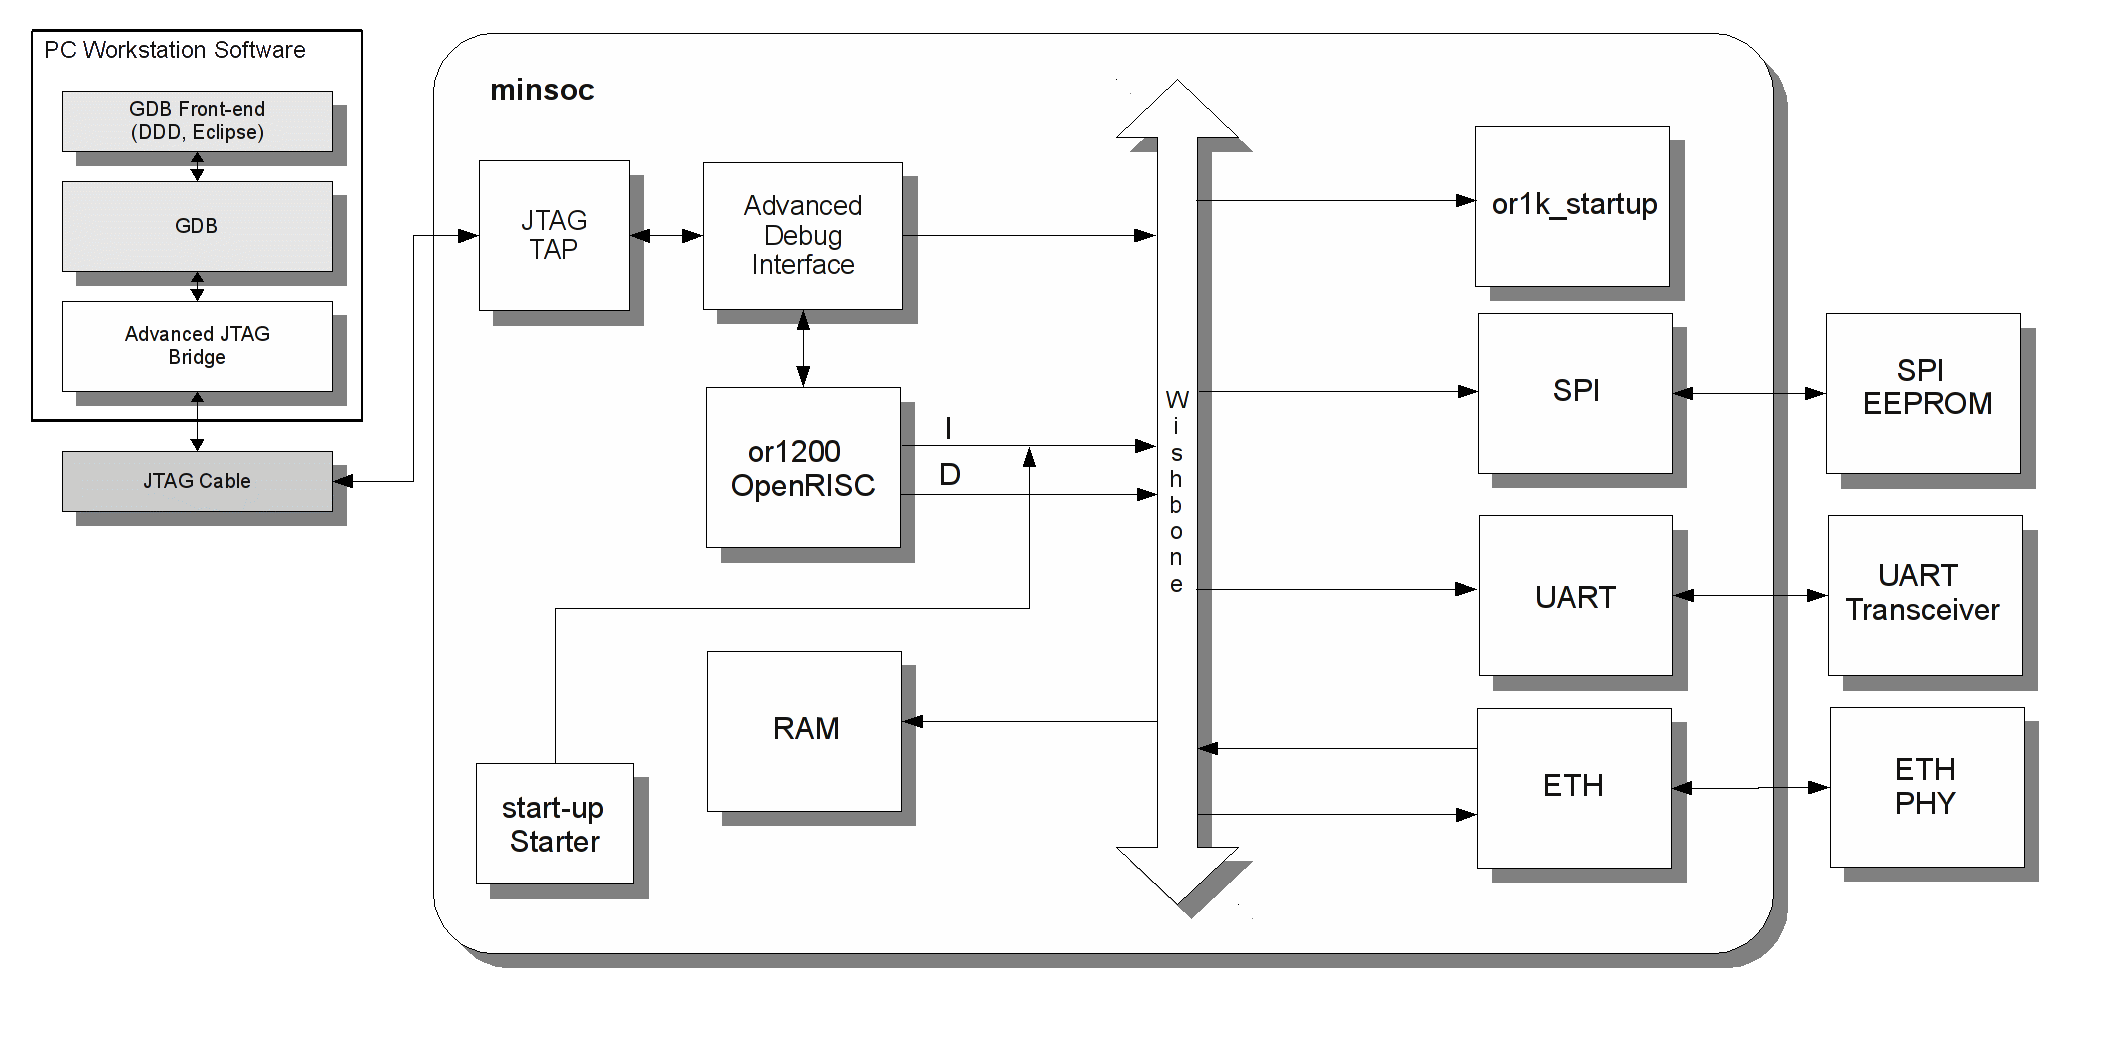
\includegraphics[width=1\textwidth,keepaspectratio=true]{./images/minsoc}
  \caption{Arquitectura MinSoc}
  \label{fig:esquemaminsoc}
 \end{center}
\end{figure}

\begin{itemize}
\item Características:
				\begin{itemize}
				  \item Microprocesador embebido OR1200 OpenRISC 
				  \item memoria redimensionalble
				  \item selección de frecuencia del sistema
				  \item JTAG debug con capacidad para distintos cables
				  \item Posibilitad de arranque automático de un firmware desde una memoria externa SPI
				  \item Modulos de UART y Ethernet 
				  \item Código genérico y especifico de memoria para las FPGA de Xilinx y Altera, adaptación de clock (PLLs y MCMs) y JTAG TAP
				  \item Configuración del sistema en un simple archivo de definición 
				  \item Ejemplos de firmware utilizando UART y Ethernet  
				  \item Incluye testbench para la simulacón de la configuración del sistema. 						
				\end{itemize}

\item Tecnologías probadas que le brindan soporte al proyecot MinSoC:


\begin{itemize}
				  \item Xilinx, Spartan 3E (Spartan3E Starter Kit)
				  \item Xilinx, Spartan 3A (Spartan3A 1800 DSP Kit)
				  \item Xilinx, Virtex 4 (ML405 board)
				  \item Xilinx, Virtex 5 (ML505 board)
				  \item Altera, Cyclone II
				  \item Altera, Cyclone II
				  \item (DE2-70 board)
				  \item Altera, Cyclone III
				  \item Altera, Cyclone IV (Bemicro SDK board) 
				  \item Altera, Stratix II						
				\end{itemize}
\end{itemize}


				\subsection{Proyecto ORPSoC}

				Este proyecto implementa una plataforma para el desarrollo OpenRISC. Está destinado a ser un entorno de desarrollo y verificación de IP cores y
				diseños de SoC. Se trata de un proyecto desarrollado con la colaboración de una de las comunidades mas importantes de hardware de código abierto
				\url{opencores.org}.


El proyecto permite tanto a usuarios nuevos como experimentados realizar diseños con un desarrollo rápido OpenRISC.Está destinado a ser un entorno de desarrollo y verificación de núcleos de propiedad intelectual y diseños SoC.Es un proyecto de desarrollo colaborativo. Como plataforma de desarrollo proporciona un entorno modular y facil de usar, para el desarrollo de código RTL y su posterior simulación y síntesis. Provee un entorno de herramientas para desarrollo de aplicaciones OpenRISC para su simulación y prueba en la placa de desarrollo.

Una visión general sobre el SoC completa y sus conexiones externas es en la  (Figura ~\ref{fig:esquemaorpspc})

\begin{figure}[h!]
 \begin{center}
  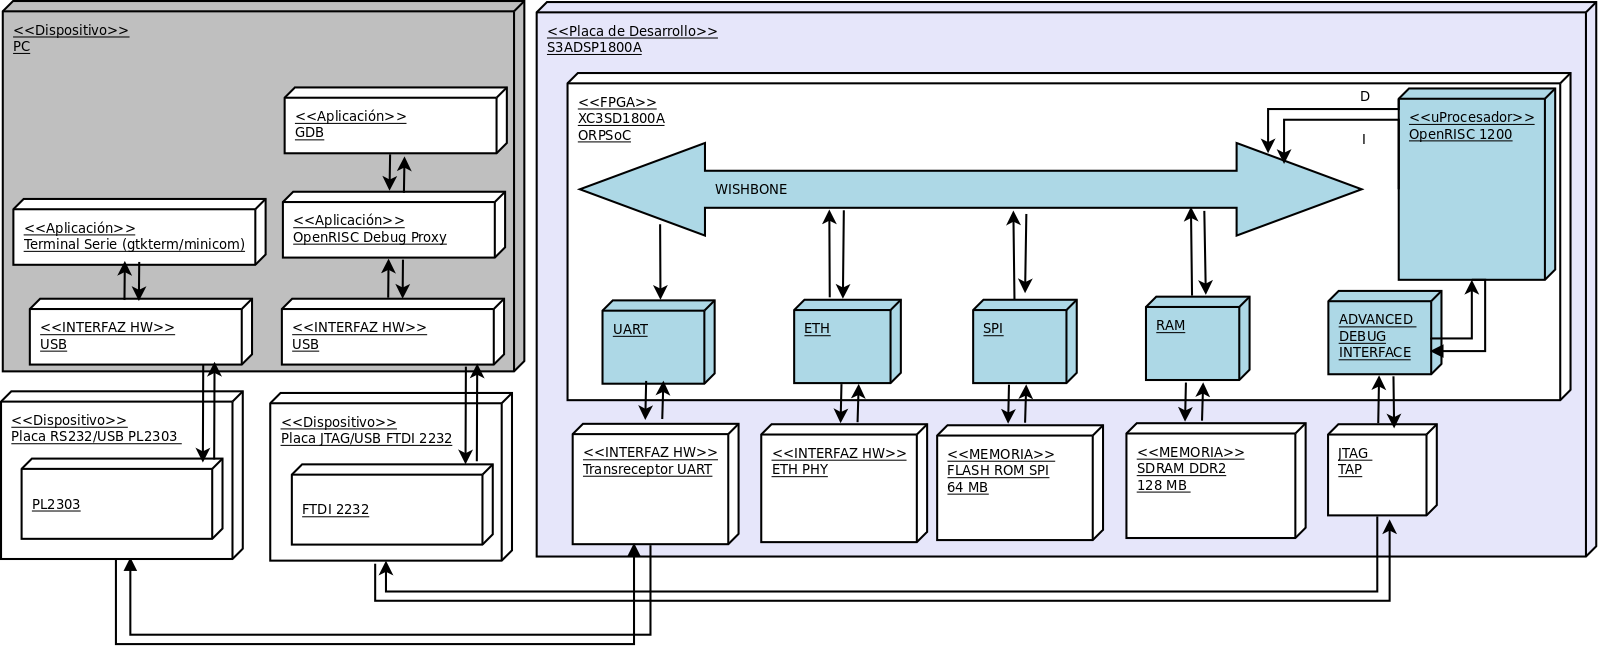
\includegraphics[width=1\textwidth,keepaspectratio=true]{./images/orpsoc}
  \caption{Arquitectura ORPsoc}
  \label{fig:esquemaorpsoc}
 \end{center}
\end{figure}

\begin{itemize}
\item Características:
				\begin{itemize}
				  \item Microprocesador embebido OR1200 OpenRISC 
				  \item memoria redimensionalble
				  \item selección de frecuencia del sistema
				  \item JTAG debug con capacidad para distintos cables
				  \item Posibilitad de arranque automático de un firmware desde una memoria externa SPI
				  \item Modulos de UART y Ethernet 
				  \item Código genérico y especifico de memoria para las FPGA de Xilinx y Altera, adaptación de clock (PLLs y MCMs) y JTAG TAP
				  \item Configuración del sistema en un simple archivo de definición 
				  \item Ejemplos de firmware utilizando UART y Ethernet  
				  \item Incluye testbench para la simulacón de la configuración del sistema. 						
				\end{itemize}

\item Tecnologías probadas que le brindan soporte al proyecot MinSoC:


\begin{itemize}
				%  \item Xilinx, Spartan 3E (Spartan3E Starter Kit)
				  \item Xilinx, Spartan 3A (Spartan3A 1800 DSP Kit)
				  %\item Xilinx, Spartan 6 LX45 (ML405 board)
				  \item Xilinx, Virtex 5 (ML501 board
					% \item Altera, Cyclone II
				  %\item Altera, Cyclone II
				  %\item (DE2-70 board)
				%  \item Altera, Cyclone III
				  \item Altera, Cyclone IV (Terasic DE0 Nano) 
				%  \item Altera, Stratix II						
				\end{itemize}
\end{itemize}

				

\section{Presentación de Placas de Desarrollo}
 
				Los proyectos MinSoC y OrpSoc cuentan actualmente con soporte para diversas placas de desarrollo. 

				\subsection{Xilinx}
				La empresa Xilinx provee kits de desarrollo de diversas características y prestaciones. A continuación se detallan algunas de las alternativas que
				son soportadas por los SoC elegidos.
				\subsubsection{S3ADSP1800A}
				El dispositivo XtremeDSP™ Starter Platform cuenta con una FPGA de la familia Spartan®-3A que permite la evaluación diseños para diferentes
				aplicaciones tales como Prototipado General, Sistemas Embebidos, Video Digital, DSP, Procesamiento de Imagenes, Comunicaciones digitales y
				Coprocesamiento. Esta plataforma provee acceso a las capacidades de la familia de FPGA Spartan®-3A y cuenta con periféricos,conectores e
				interfaces estándar de la industria. Fue diseñada para para ser utilizada con Xilinx System Generator para aplicaciones DSP y las herramientas de
				diseño ISE® o el entorno desarrollado en Linux llamado PetaLinux Software Development Kit (SDK) ambas herramientas provistas por el fabricante. 
				
				%Traducir esto ???
				Las características generales del kit son:
			
				\begin{tabular}{ p{4cm} p{10cm} }
				\rowcolor[gray]{0.8} Caracteristica & Descripción \\		
				\hline FPGA   & XC3SD1800A-4FGG676C Spartan-3A DSP FPGA\\
				\hline Clocks & 125 MHz LVTTL SMT oscillator\\
				\hline        & LVTTL oscillator socket\\
				\hline		  & 25.175 MHz LVTTL SMT oscillator (video clock)\\
				\hline		  & 25 MHz Ethernet clock (accessible to FPGA)\\
				\hline Memory & 128 MB (32M x 32) DDR2 SDRAM\\
				\hline		  & 16Mx8 parallel / BPI configuration flash\\
				\hline 		  & 64 Mb SPI configuration / storage flash (with 4 extra SPI selects)\\
				\hline Interfaces & 10/100/1000 PHY\\
				\hline			  & JTAG programming/configuration port\\
				\hline            & RS232 Port\\
				\hline			  & Low-cost VGA\\
				\hline			  & 4 SPI select lines\\
				\hline Buttons and Switches & 8 user LEDs\\
				\hline  		  & 8-position user DIP switch\\
				\hline            & 4 user push button switches\\
				\hline 			  & Reset push button switch\\
				\hline User I/O and Expansion & Digilent 6-pin header\\
				\hline			 			  & EXP expansion connector\\
				\hline 						  & 30-pin GPIO connector: can be used for System ACE™ Compact Flash daughter card (not included)\\
				\hline Configuration and Debug & JTAG\\
				\hline                         & System ACE module connector\\   
				\end{tabular}
				
				Las implementaciones MinSoC y ORPSoC proveen soporte nativo para los siguientes periféricos:
				
				\begin{itemize}
				  \item Ethernet
				  \item GPIO (Solo ORPSoC)
				  \item DDR2 SDRAM (128MB) (Solo ORPSoC)
				  \item SPI
				  \item UART				
				\end{itemize}
			
				\subsubsection{ML501}
				La ML501 es una plataforma de desarrollo de bajo costo y gran funcionalidad que provee un acceso práctico a los recursos disponibles en el
				dispositivo FPGA Virtex®-5 LX50. Posee interfases y conectores industriales estándar y presenta gran versatilidad para su utilización en
				múltiples aplicaciones como Video, Audio y puertos de comunicación.
				
				Las características generales del kit son:
			
			\begin{tabular}{ p{4cm} p{10cm} }
			\rowcolor[gray]{0.8} Caracteristica & Descripción \\		
			\hline FPGA & XC5VLX50FFG676\\
			\hline Memoria & DDR2 SODIMM (256 MB)\\
			\hline 		   & ZBT SRAM (1 MB)\\
			\hline 		   & Linear Flash (32 MB)\\
			\hline         & System ACE™ CF technology (Compact Flash)\\
			\hline         & Platform Flash\\
			\hline         & SPI Flash\\
			\hline Clocks  & External clocking (2 differential pairs)\\
			\hline Interfaces & USB (2) - host and peripheral\\
			\hline 			  & PS/2 (2) - keyboard, mouse\\
			\hline 			  & RJ-45 - 10/100 Networking\\
			\hline 			  & RS-232 (male) - serial port\\
			\hline 			  & Audio In (2) - line, microphone\\
			\hline 			  & Audio Out (2) - line, amp, SPDIF, piezo speaker\\
			\hline 			  & Video (DVI/VGA) Output\\
			\hline I/O y expansión & Single-ended and differential I/O expansion\\
			\hline GPIO		&  DIP switch (8)\\
			\hline 			&  LEDs (8)\\
			\hline 			&  push buttons (5)\\
			\hline Debug y programación & JTAG programming interface\\
			\hline Medioambiente & EU-RoHS compliant \\
			\end{tabular}
				
				Las implementación ORPSoC fue probada con éxito en esta plataforma y provee soporte para los siguientes periféricos:
				
				\begin{itemize}
				  \item Ethernet
				  \item GPIO
				  \item DDR2 SDRAM (256MB)
				  \item CFI flash (32MB)
				  \item SRAM
				  \item SPI
				  \item UART
				  \item AC97 
				  \item PS/2 				
				\end{itemize}
			
				
				\subsection{Digilent}
				\subsubsection{Atlys}
				La placa de desarrollo Atlys es una plataforma que permite el desarrollo de circuitos digitales y esta soportada por una FPGA Xilinx Spartan 6 LX45. Posee periféricos entre los que se destacan Gbit Ethernet, Video HDMI, Audio, puertos USB y Memoria Ram 128 MB DDR2 que permiten el
				desarrollo de Sistemas Digitales sobre procesadores embebidos como  MicroBlaze de Xilinx. Atlys es compatible con todas las herramientas CAD de
				Xilinx como ChipScope, EDK y WebPack (gratuito) lo que permite completar diseños sin mayor costo. Como alternativa puede utilizarse un entorno de
				desarrollo para Linux llamado PetaLinux Software Development Kit (SDK) provisto por el fabricante de la FPGA.
				
				Las características generales de la plataforma son:
				
				\begin{tabular}{ p{4cm} p{10cm} }
				\rowcolor[gray]{0.8} Caracteristica & Descripción \\		
				\hline FPGA   & Spartan-6 LX45, 324-pin BGA package \\
				\hline 		  &	6,822 slices each containing four 6-input LUTs and eight flip-flops\\
				\hline DSP	  & 58 DSP slices\\
				\hline Clocks & 2.1Mbits of fast block RAM\\
				\hline 		  & 4 clock tiles (8 DCMs \& 4 PLLs)\\
				\hline 		  & 6 phased-locked loops\\
				\hline 		  & 500MHz+ clock speeds\\
				\hline 		  & 100MHz CMOS oscillator\\
				\hline Memoria & 128Mbyte DDR2 16-bit wide data\\
				\hline         & 16Mbyte x4 SPI Flash for configuration \& data storage\\
				\hline GPIO & 8 LEDs \\
				\hline 		& 6 buttons\\
				\hline		& 8 slide switches\\
				\hline Interfaces & 10/100/1000 Ethernet PHY\\
				\hline 			  & On-board USB2 ports for programming \& data transfer\\
				\hline 			  & USB-UART and USB-HID port (for mouse/keyboard)\\
				\hline 			  & Two HDMI video input ports \& two HDMI output ports\\
				\hline			  & AC-97 Codec with line-in, line-out, mic, \& headphone\\
				\hline Energía & Real time power monitors on all power rails\\
				\hline 		   & 20W power supply and USB cable\\
				\hline I/O y Expansión & 48 I/O’s routed to expansion connectors\\
				\end{tabular}
				
				La implementación ORPSoC proveen soporte nativo para los siguientes periféricos:
				
				\begin{itemize}
				  \item AC97
				  \item Ethernet
				  \item GPIO
				  \item PS/2 
				  \item DDR2 SDRAM (128MB)
				  \item SPI
				  \item UART
				  \item VGA
				\end{itemize}				

				\subsection{Terasic}
				\subsubsection{Terasic DE0 Nano}
				La plataforma DE0-Nano posee un tamaño compacto que se ajusta al diseño de circuitos para proyectos portables. Fue diseñada para ser
				utilizada con una implementación simple utilizando como destino una FPGA Cyclone IV de Altera con 22,320 LEs (Elementos Lógicos). Entre sus
				características princpiales se encuentran diversas interfases que incluyen dos puertos de expanxión GPIO, dispositivos de memoria on board SDRAM y
				EEPROM. Las mayores ventajas del DE0-Nano son su reducido tamaño y peso, así como la capacidad de ser reconfigurado sin la necesidad de
				utilización de hardware extra. Los requerimientos de energía para dispositivos portables son cruciales , la DE-0 Nano posee 3 esquemas posibles
				de conexión : un puerto USB mini-AB, conectores de 2 pines para alimentación externa de 5V, y 2 pines de 5V.

				Las características generales de la plataforma son:
				
				\begin{tabular}{ p{4cm} p{10cm} }
				\rowcolor[gray]{0.8} Caracteristica & Descripción \\		
				\hline FPGA   	& Cyclone® IV EP4CE22F17C6N FPGA\\
				\hline 			& 22,320 Logic elements (LEs)\\
				\hline 			& 594 Embedded memory (Kbits)\\
				\hline 			& 66 Embedded 18 x 18 multipliers\\
				\hline			& 4 General-purpose PLLs\\
				\hline 			& 153 Maximum FPGA I/O pins\\ 
				\hline Configuration Status and Set-Up Elements & 	On-board USB-Blaster circuit for programming\\
				\hline											&	FPGA Serial Configuration Device (EPCS)\\
				\hline Expansion Header & 	Two 40-pin Headers (GPIOs) provides 72 I/O pins\\
				\hline 					&	Two 5V power pins, two 3.3V power pins and four ground pins\\
				\hline 					&	One 26-pin header provides 16 digital I/O pins and 8 analog input pins to connect to analog sensors, etc\\ 
				\hline Memory Devices	&	32MB SDRAM\\
				\hline 					&	2Kb I2C EEPROM\\ 
				\hline General User Input/Output 	& 8 green LEDs\\
				\hline 								& 2 debounced push-buttons\\
				\hline 								& 4 dip switches\\ 
				\hline G-Sensor & ADI ADXL345, 3-axis accelerometer with high resolution (13-bit)\\ 
				\hline A/D Converter & NS ADC128S022, 8-Channel, 12-bit A/D Converter\\ 
				\hline					 & 50 ksps to 200 ksps \\
				\hline Clock System & On-board 50MHz clock oscillator\\
				\hline Power Supply & USB Type mini-AB port (5V)\\
				\hline 				& Two DC 5V pins of the GPIO headers (5V)\\
				\hline 				& 2-pin external power header (3.6-5.7V)\\
				\end{tabular}
				
				La implementación ORPSoC proveen soporte nativo para los siguientes periféricos:
				
				\begin{itemize}
				  	\item GPIO
					\item SDRAM (32MB)
					\item UART
					\item SPI FLASH (8MB)
					\item I2C
				\end{itemize}				
				
 		\subsection{Conclusiones de la elección de la Placa de Desarrollo}
 				Se seleccionó entre los items analizados y teniendo en cuenta la disponibilidad de recursos al momento de realizar este trabajo utilizar las
 				placas S3ADSP1800A de Xilinx para soportar los SoC a implementar.
 		
 		\newpage	
 		\section{Presentación de las herramientas de desarrollo} 	 
 				\subsection {Herramientas de Desarrollo de Hardware}
 				Durante el proceso de desarrollo e implementación de hardware mediante lógica programable son necesarias un serie de herramientas que
 				proporcionan diferentes salidas en cada etapa del proceso. En la Figura ~\ref{fig:designflow} se observan las etapas del flujo de diseño y sus
 				respectivas salidas.
 				
 		\begin{figure}[h!]
 		\begin{center}
  		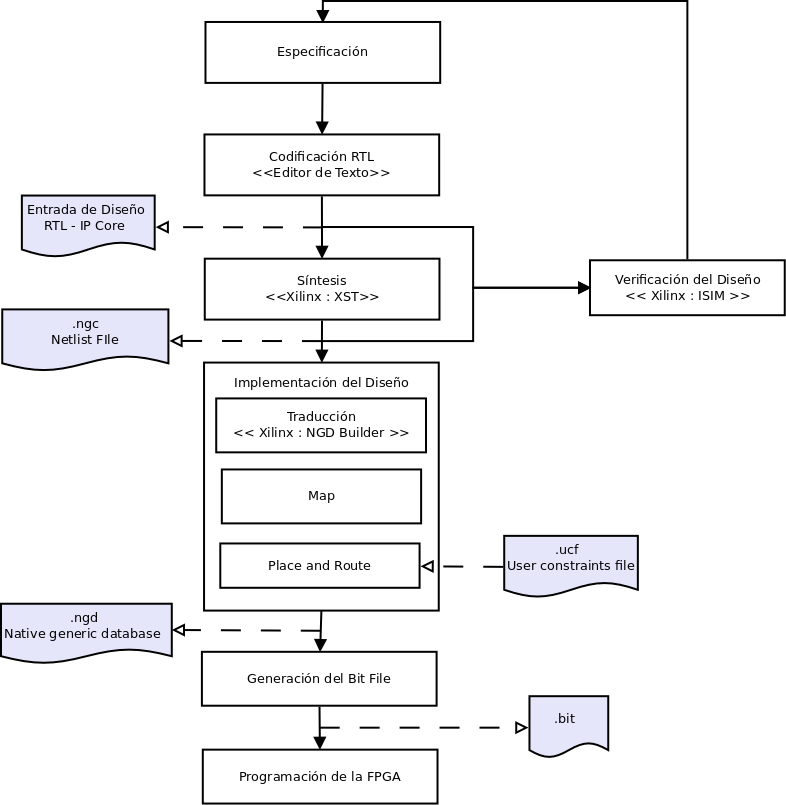
\includegraphics[width=0.7\textwidth,keepaspectratio=true]{./images/designflow}
  		\caption{Flujo de diseño e implementación de hardware con lógica programable}
  		\label{fig:designflow}
 		\end{center}
		\end{figure}
		
				Se analizaron las aplicaciones alternativas para cada etapa, enfatizando la selección de aplicaciones que cumplan con el requerimiento RQX-LC 2
				planteado en la Tabla ~\ref{tab:requsr2}.   
				
				\subsubsection {Codificación RTL - Editores de Texto}
				Existen diversas herramientas de Edición de Texto que poseen características compatibles con el desarrollo de código de descripción de hardware.
				Entre las características más comunes encontramos numeración de líneas, resaltado de código, y predictores. 
				Xilinx provee en su Suite de Desarrollo la posibilidad de confeccionar código directamente desde ISE Project Mananger. Sin embargo,
				existen alternativas Open Source de capacidades comparables tales como emacs o gedit. 
				
				\subsubsection {Síntesis, Implementación del Diseño y Generación del Bit File}
				En estas etapas del proceso de diseño no existen herramientas alternativas con licencias OpenSource que permitan obtener el archivo de
				configuración de la FPGA. Esta restricción obliga a los desarrolladores a utilizar solo las herramientas del fabricante al implentar sus diseños
				en FPGA.
				Para realizar la síntesis, Xilinx, utiliza la aplicación XST que realiza la traducción de la descripción RTL escrita en algún lenguaje de
				descripción de Hardware como Verliog o VHDL en una lista de elementos lógicos y sus conexiones. La siguiente etapa consiste en la implementación 
				del diseño y consta de tres grandes etapas: Translate, Map, Place and Route. Finalizada esta etapa se obtiene el diseño adecuado al modelo de
				fpga seleccionado, sus clocks y sus conexiones de entrada/salida. 
				
				\subsubsection {Programación y Configuración de la FPGA}
				La acción que culmina el proceso de implementación es la descarga del código binario de configuración en la FPGA. El protocolo utilizado para
				realizar esta acción se denomina JTAG (Joint Test Action Group) se encuentra implementado en diversos dispositivos de programación de FPGA y
				microprocesadores. La mayoría de estos dispositivos proveen soporte SPI (Serial Peripheral Interface) que permite el acceso a dispositivos de
				almacenamiento como lo son, por ejemplo, las memorias Flash SPI.
				
				Xilinx provee la aplicación iMPACT con su Suite de Desarrollo ISE. Esta herramienta es compatible con todos los dispositivos fabricados por
				Xilinx y algunos dispositivos incluídos en sus placas de prueba. Durante el desarrollo de este trabajo los autores debieron lidiar con
				problemas de acceso a dispositivos de terceros que conforman la placa de desarrollo S3ADSP1800A que produjeron retrasos significativos en
				realización del proyecto.
 				
 				Alternativamente, existen herramientas Open Source tales como XC3SPROG y UrJTAG , ambos licenciados bajo GPLv2 . La herramienta XC3SPROG
 				posee capacidades comparables al iMPACT y proporciona acceso de diversos disposivitos entre los que se encuentran:
 				\begin{itemize}
 				  \item Dispositivos Xilinx
				  \item Dispositivos Atmel 
				  \item Memorias SPI flash: AT45, AMIC, AMIC-QUAD, M25P, N25Q, S33, W25
 				\end{itemize}
 				 
 				\subsection {Herramientas de Desarrollo de Software}
 			
				Se analizaron las aplicaciones alternativas para cada etapa, enfatizando la selección de aplicaciones que cumplan con el requerimiento RQX-LC 3
				planteado en la Tabla ~\ref{tab:requsr2}.   
				 			
 				\subsubsection {Toolchain para OpenRISC}
 				La comunidad OpenCores realizó una adapatación del Toolchain GNU para generar aplicaciones en C y C++ que se ejecuten en una arquitectura
 				OpenRISC. Así mismo fueron adaptadas las librerias newlib y uClibc conformando una solución completa al diseño y desarrollo de aplicaciones
 				OpenRISC. Existe un entorno de desarrollo gráfico llamado OpenIDEA desarrollado por Dynalith basado en este toolchain. 
				
				El proyecto OpenRISC cuenta con un simulador del repertorio de instrucciones llamado or1ksim que permite la simulación de aplicaciones compiladas
				mediante el toolchain sin necesidad de tener disponible el hardware de prueba durante la etapa de desarrollo de software.
 				
 	

		\section{Presentación de los Sistema Operativo}
 		
			 	\subsection{ecOS}

eCos \cite{Etiqueta35} es un sistema operativo de tiempo real y de código abierto para aplicaciones embebidas, y es desarrollado por eCosCentric, una división de RedHat. Según el autor eCos es el RTOS más popular en la actualidad y ha sido utilizado en varios productos como 
por ejemplo receptores de radio satelital Sirius, módulos Wi-Fi de la consola Sony PlayStation 3 
y routers Netgear, entre otros. 


 eCos viene de "Embedded Configurable Operating System", y según sus creadores puede ser configurado para ejecutarse tanto en dispositivos con memoria muy limitada de tipo SoC (System on a Chip) como en sistemas más complejos que requieren mayores funcionalidades. 
 
El sistema es distribuído sin costo bajo licencia GPL modificada, la cual permite el uso de código propietario en conjunto con eCos. Esto significa que la licencia no requiere que el código desarrollado sobre eCos sea necesariamente de tipo GPL. También existe una versión comercial 
(eCosPro).

Características generales: 
				\begin{itemize}
				  	\item Algoritmo de itineración de tipo Round Robin
					\item Kernel de tipo apropiativo o cooperativo (configurable). Pueden añadirse schedulers 
 adicionales
					\item El Kernel no desactiva las interrupciones
					\item Implementación de mutexes, semáforos binarios y de conteo, variables de condición, 
 casillas de correo, banderas de evento y spinlocks
					\item Memory Allocation: Fixed Block, Variable Block and dynamic heaps. (configurable)
					\item Bibliotecas disponibles ISO C y Math, C++/STL, microITRON y POSIX. 
					\item  Incluye un pequeño stack IP
					\item Sistema de Archivos FAT12/16/32
					\item Incluye un bootloader con opciones de debugging
				\end{itemize}			

Arquitecturas compatibles:

				\begin{itemize}
				\item x86 / i386 / IA-32
				\item x86 Multiprocesamiento simétrico
				\item x86-64
				\item PowerPC Multiprocesamiento simétrico
				\item Alpha
				\item ARM
				\item Intel XScale
				\item M68k
				\item PA-RISC
				\item OpenRISC
				\item CalmRISC
				\item Nios II
			\end{itemize}			

	

			 \subsection{Linux}

El sistema operativo Linux es una implementación de libre distribución UNIX para computadoras personales (PC), servidores, y estaciones de trabajo.Como sistema operativo, Linux es muy eficiente y tiene un excelente diseño.





 
Características generales:

	\begin{itemize}
	\item Licencia de Software: GPL/LGPL
	\item Tipo de núcleo: núcleo monolítico con módulo
	\item Lenguaje de programación del núcleo en c
	\item Soporte de Hilo de ejecución del núcleo: 1:1
	\item Familia de SO tipo UNIX
	\item Comunicación entre procesos y sincronización
	\item Multitarea
	\item Unidad de Gestión de Memoria 
	\item Tecnología de red TCP/IP,IPv6, IPX, PPP, PPPoE, DHCP, bridge, TUN/TAP, ssh, OpenVPN 	
	\item Sistema de archivos NTFS,ext2, MS-DOS, FAT16/32 y otros
	\item Forks: microCLinux	
	
\end{itemize}			

Arquitecturas compatibles:

				\begin{itemize}
				\item x86 / i386 / IA-32
				\item x86 Multiprocesamiento simétrico
				\item Xen
				\item IA-64 	
				\item SPARC32
				\item x86-64
				\item PowerPC
				\item PowerPC Multiprocesamiento simétrico
				\item Alpha
				\item MIPS
				\item ARM
				\item Intel XScale
				\item M68k
				\item PA-RISC
				\item OpenRISC
			\end{itemize}			

%Hardware compatible:

%			\begin{itemize}
%				\item ATA
%				\item SATA
%				\item SCSI
%				\item USB 2.0 	
%				\item USB 1.1
%				\item FireWire
%				\item PCMCIA/PC card
%				\item AGP
%				\item Nvidia official driver IA32
%				\item Nvidia official driver IA64
%				\item Nvidia official driver AMD64
%				\item ATI official driver x86
%				\item ATI official driver x86-64
%				\item Ati r200 free software driver
%				\item Ati r300 free software driver
%				\item Nvidia free software driver
%				\item Audio
%			\end{itemize}
%Interconexión:

%			\begin{itemize}
%				\item Networking supported	
%				\item NE2000/RTL8029
%				\item RTL8139
%				\item Gigabit Ethernet 	
%				\item 10 Gigabit Ethernet
%				\item WLAN
%				\item Bluetooth
%				\item IrDA
%			\end{itemize}

%Tecnologías de red:

%			\begin{itemize}
%				\item Firewall: netfilter/iptables
%				\item TCP/IP	
%				\item IPv6
%				\item IPX 	
%				\item PPP			
%				\item PPPoE
%				\item DHCP
%				\item bridge
%				\item TUN/TAP
%				\item ssh
%				\item OpenVPN
%			\end{itemize}

%Sistemas de archivos compatibles:


%			\begin{itemize}
%				\item FAT16 dosfs, FAT32/vfat	
%				\item NTFS	
%				\item Ext2	
%				\item Ext3	
%				\item XFS	
%				\item ReiserFS	
%				\item UFS	
%				\item UFS2	
%				\item HFS
%				\item HFS+	
%				\item Minixfs	
%				\item BFS	
%				\item ISO 9660	 
%				\item UDF	
%				\item NFS	
%				\item SMBFS	
%				\item Disco RAM/tmpfs	
%				\item procfs	
%				\item Memoria virtual/Swap	
				
%			\end{itemize}


		\subsection{ BusyBox}	
 	
				
			 
BusyBox \cite{Etiqueta36} combina versiones de varias utilidades comunes de UNIX en un sólo ejecutable. Remplaza las utilidades que se suelen encontrar en fileutils GNU, shellutils, etc. Las utilidades en BusyBox tiene menos funciones que GNU, sin embargo, las opciones que incluyen proporcionan la funcionalidades necesarias. BusyBox proporciona un entorno  completo para cualquier sistema pequeño o embebido.

Este conjunto de programas están optimizados de acuerdo a las limitaciones de los recursos disponibles de hardware. También se puede fácilmente incluir o excluir comandos (o características) en tiempo de compilación. Esto hace que sea fácil de personalizar un sistemas embebidos. 

%Para crear un sistema de trabajo, sólo tiene que añadir algunos nodos de dispositivos en / dev, algunos archivos de configuración en / etc, y un núcleo de Linux.

BusyBox es mantenida por Denys Vlasenko, y licenciado bajo la GNU GPL.

%%%%%%%%%%%%%%%%%%%%%%%%%%%

			
 			
 
%%%%%%%%%% OPENRISC   %%%%%%%%%%%%%%%%
\chapter{Análisis del microprocesador OpenRISC}
	\section{Introducción}
	El proyecto OpenRISC apunta al desarrollo de arquitecturas RISC de propósito general. OpenRISC 1000, desarrollada por OpenCores, describe una
	familia de procesadores de 32 y 64-bits con procesamiento opcional de punto flotante y vectores.\cite{etiqueta_OR_01}. Su primera implementación
	llamada OpenRISC 1200 (OR1200), escrita en Verilog fue diseñada bajo licencia LGPL con modelos y firmware bajo licencia GPL. 
	
	El OR1200 es un RISC escalar con microarquitectura Harvard, un pipeline de enteros de 5 etapas, soporte de memoria virtual (MMU) y capacidades DSP
	básicas. Las memorias cache por defecto son directas, de 1 vía con 8KB de datos y 1 vía con 8KB de instrucciones respectivamente, cada  una con
	16-bytes de tamaño de línea. Son implementadas inicialmente y constituidas por un TLB de datos de 1 vía y 64 entradas basada en hash en conjunto con
	una TLB de instrucciones de 1 vía y 64 entradas basada en hash. Incluye una unidad de debug de tiempo-real, tick timer, controlador de interrupciones
	programable y soporte para el manejo de energía. La mayoría de sus características pueden ser configuradas por el usuario.
		
	\section{Arquitectura}
	
	La arquitectura OR1000 se basa en la arquitectura del DLX, que es similar a la arquitectura del primer MIPS (MIPS-I). Posee un espacio de direcciones
	lógicas lineal de 32 o 64 bits y espacio de direcciones físicas de implementación opcional. Utiliza un formato de instrucciones simple y de largo
	uniforme en 4 versiones:
	
	\begin{itemize}
	  \item  Set de instrucciones Básico de OpenRISC (ORBIS 32/64) con instucciones de 32 bits alineados en memoria operando con datos de 32 o 64
	  bits.
	  \item Extensión para vectores y DSP (ORVDX64) con instrucciones de 32 bits alineados en memoria operando con datos de 8,16,32 y 64 bits.
	  \item Extensión de punto flotante (ORFPX32/64) con instrucciones de 32 bits alineados en memoria y operandos de 32 y 64 bits.  
	\end{itemize}
	
	Posee dos modos de direccionamiento de memoria: la primera mediante la suma de un operando registro y un inmediato de 16 bits mientras que la segunda
	se realiza sumando un operando registro y un inmediato de 16 bits seguido de una actualización del operando registro con la dirección efectiva
	calculada. La mayor parte de las instrucciones tienen 2 operandos registro (o un registro y una constante). Utiliza retardo de salto (branch delay
	slot) para mantener el pipeline lo mas completo posible. Provee soporte para caches/MMUs de datos e instrucciones separadas (Arquitectura Harvard) y
	para caches/MMUs de datos e instrucciones unificadas (Arquitectura Stanford). Soporta cambios de contexto rápidos en registros, caches y MMUs.
	  
	La arquitectura general consiste en una serie de bloques presentados en la figura ~\ref{fig:ArqOR1200}.
		
	\begin{figure}[h!]
 	\begin{center}
  	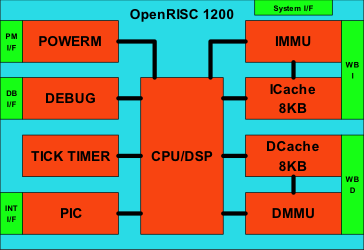
\includegraphics[width=0.5\textwidth,keepaspectratio=true]{./images/OR1200}
  	\caption{Arquitectura del OR1200}
  	\label{fig:ArqOR1200}
 	\end{center}
	\end{figure}

	\subsection{Bloque central CPU/FPU/DSP}

	
	La figura ~\ref{fig:cpufpudsp} muestra el diagrama del bloque básico de CPU/DSP , no se muestras los componentes de la FPU. El OR1200 solo
	implementas secciones de los ISA ORBIS32 y ORFPX32. 

	
	\begin{figure}[!h]
 	\begin{center}
  	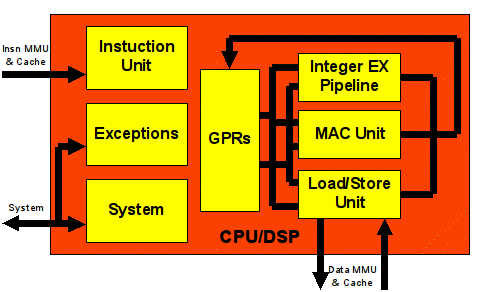
\includegraphics[width=0.5\textwidth,keepaspectratio=true]{./images/cpu_fpu_dsp}
  	\caption{Bloque central del OpenRISC 1200}
  	\label{fig:cpufpudsp}
 	\end{center}
	\end{figure}
	
	\subsection{Cache de datos}
	En la configuración por defecto se tiene una Cache directa de 1 vía con 8KB de extensión. Sin embargo ésta puede ser configurada en alguno de los
	modos listados en la tabla ~\ref{tab:cachedatos} 
	
		\begin{tabular}{ p{10cm} p{5cm}}
		\rowcolor[gray]{0.8} Modo & Espacio\\
		\hline 
		16B/linea, 256 lines, 1 vía & 4KB\\
		\hline
		16B/linea, 512 lines, 1 vía & 8KB (por defecto)\\
		\hline
		16B/linea, 1024 lines, 1 vía & 16KB\\
		\hline 
		32B/linea, 1024 lines, 1 vía & 32KB\\
		\hline
		\caption{Modos de configuración de la cache de datos del OR1200}
		\label{tab:cachedatos}
		\end {tabular}
	\subsection{Direct-mapped instruction cache}
	
	
	
	\subsection{Data MMU based on hash based DTLB}
	
	
	\subsection{Instruction MMU based on hash based ITLB}
	
	
	\subsection{Power management unit and power management interface}
	
	
	\subsection{Tick timer}
	
	
	\subsection{Debug unit and development interface}
	
	
	\subsection{Interrupt controller and interrupt interface}
	
	
	\subsection{Instruction and Data WISHBONE host interfaces}
	
	
	
	\section{Set de instrucciones}
	
	
	
	\section{Implementación}
		\subsection{ORPSoC}
		\subsection{MinSoc}
	\section{Toolchain}
	\section{Software}
		\subsection{Librerías}
		\subsection{Sistema Operativo} % OpenRisc
\newpage
%%%%%%%%%%%%%%%%%%%%%%%%%%%%%%%%%%%%%%%%% CAPITULO 3 %%%%%%%%%%%%%%%%%%%%%%%%%%%%%%%%%
\chapter{Benchmarking}
	\section{Introducción}
	En informática benchmark representa la acción de ejecutar un programa de computadora, un conjunto de programas, u otras aplicaciones con el fin
	de evaluar el rendimiento relativo de un objeto, normalmente mediante la ejecución de una serie de pruebas estándar.  El Benchmarking se asocia
	generalmente con la evaluación de las características de rendimiento del hardware, por ejemplo, el rendimiento de operaciones de punto flotante de la
	CPU pero hay circunstancias en que la técnica también es aplicable al software. Los benchmarks de software son ejecutados para evaluar el
	rendimiento de compiladores o sistemas de gestión de bases de datos .
	
	Los Benchmarks proveen un método de comparación de las prestaciones de varios subsistemas que conforman la arquitectura de un sistema. Debido a que
	las arquitecturas de computadoras se han vuelto cada vez más complejas, resulta difícil comparar las prestaciones de varios sistemas de computadoras
	con simplemente evaluar sus especificaciones. Es necesario entonces la utilización de tests que permitan la comparación de diferentes arquitecturas.
	Por ej., los procesadores Pentium 4 de Intel generalmente operaban a mayor frecuencia que los Athlon XP de AMD, lo que no necesariamente debía
	interpretarse como una mayor capacidad de procesamiento.
	
	Son diseñados para imitar una clase particular de carga de trabajo en un componente del sistema. Los benchmarks sintéticos realizan esto mediante
	programas especialmente creados para dirigir la carga de trabajo en un compenente específico. Los benchmarks de aplicaciones ejecutan programas
	de uso cotidiano de los usuarios. Mientras los benchmarks de aplicaciones generalmente proporcionan una mejor medición de la performace del sistema
	respecto de aplicaciones cotidianas, los benchmarks sintéticos son más efectivos para probar compenentes individuales como discos rígidos o
	dispositivos de red.

	Los benchmarks tienen gran importancia en el diseño de CPUs, proveyendo a los diseñadores la habilidad de medir y realizar compartivas duranta las
	decisiones respecto a la microarquitectura. Hasta el año 2000 utilizaban el benchmark de Standard Performance Evaluation Corporation (SPEC) aunque
	las versiones SPEC para sistemas operativos Unix eran aún de gran tamaño y difíciles de usar sin modificar.
	
	Es sabido que algunos fabricantes de computadoras modificaron sus sistemas para mostrar altos indicadores de performace luego de la ejecución de los
	tests benchmark que no eran reflejados luego durante la ejecucción real de aplicaciones. Durante los 80' algunos compiladores detectaban una
	operación matematica específica utilizada en los benchmarks de punto flotante mas conocidos y reemplazaban la misma con una operacion matemática
	equivalente de ejecución más rápida. Sin embargo, esta transformación rara vez era útil en la ejecución de programas fuera del benchmark hasta que a
	mediados de los 90', cuando las arquitecturas Reduced instruction set computing (RISC) y Very long instruction word (VLIW) enfatizaron la importancia
	de los compiladores en lo relativo a la performace. Actualmente, los benchmarks son utilizados por los desarrolladores de compiladores para
	incrementar no solo sus indicadores de benchmark sino también su performance en aplicaciones reales. Las CPUs que poseen mas unidades de ejecución
	usualmente completan tareas reales y de benchmark en menos tiempo que los supuestos más rápidos, procesadores de mayores frecuencias de clock.
	
	\section{Tipos de Benchmarks}
	Como se ha mencionado en el apartado anterior existen diferentes tipo de benchmarks que permiten obtener un valor cuantitativo de la performace de un
	componente en diferentes circunstancias de ejecución.
	
		\begin{tabular}{ p{2.5cm} p{8cm} p{3cm} }
		\hline 
		\rowcolor[gray]{0.8} Tipo & Descripción & Ejemplo \\
		\hline
		De programas reales  &  Diseñados para evaluar el rendimiento de el procesador en aplicaciones de uso cotidiano: procesadores de texto
		como \LaTeX, software de diseño asistido por computadora (CAD) y aplicaciones generales de usuario \& SPECint y SPECfp\\
		\hline
		Microbenchmark  &  Diseñados para medir la performance de una pequeña y específica porción de código \\
		\hline
		Kernel			&  Se basan en el análisis y conocimiento de que en la mayoría de los casos solo el 10 \% del código ejecutado utiliza el 80\% de los
		recursos de CPU utilizando estas porciones de código clave para realizar el benchmark.\cite{EtiquetaBM01} & linpack y livermore loops\\
		\hline
		Benchmark de componentes & Programas diseñados para medir la performance de componentes básicos. Detectan automáticamente parametros de hardware
		como el numero de registros, tamaño de cache, latencia de memoria,etc. &  SPEC CPU2006\\
		\hline
		
		\end{tabular}
	
	Component Benchmark/ micro-benchmark
		programs designed to measure performance of a computer's basic components [3]
		automatic detection of computer's hardware parameters like number of registers, cache size, memory latency
	Synthetic Benchmark
		Procedure for programming synthetic benchmark:
			take statistics of all types of operations from many application programs
			get proportion of each operation
			write program based on the proportion above
	
		Types of Synthetic Benchmark are:
			Whetstone
			Dhrystone
		These were the first general purpose industry standard computer benchmarks. They do not necessarily obtain high scores on modern pipelinedcomputers.
	I/O benchmarks
	
	Database benchmarks: to measure the throughput and response times of database management systems (DBMS')
	Parallel benchmarks: used on machines with multiple cores, processors or systems consisting of multiple machines
	
	\section{Benchmarking de Sistemas Embebidos}
	The Embedded Microprocessor Benchmark Consortium (EEMBC) develops benchmark software to help system designers select the optimal processors, and
	benchmark tools to help consumers and IT professionals select the appropriate smart phones/tablets and networking firewall appliances. EEMBC
	organizes its benchmark suites targeting Automotive, Digital Media, Java, Multicore Processors, Networking, Office Automation, Signal Processing,
	Smartphones/Tablets and Browsers.
 	
	\section{CPU core benchmarking}
 	A pesar de que no se corresponde con la forma en que utilizaría un procesador en una aplicación real , a veces es importante aislar el núcleo de la
 	CPU de los otros elementos del procesador y centrarse en un elemento clave. Por ejemplo , es posible que desee tener la capacidad de hacer caso
 	omiso de la memoria y los efectos de E / S y se centran principalmente en la operación de el pipeline. Este es el dominio de CoreMark . CoreMark es
 	capaz de probar la estructura de pipeline básica de un procesador , así como la capacidad de prueba de lectura / escritura de operaciones básicas ,
 	operaciones de enteros y operaciones de control

	\section{CoreMark}

	CoreMark es un punto de referencia que tiene como objetivo medir el rendimiento de las unidades centrales de procesamiento ( CPU) utilizados en
	sistemas embebidos. Fue desarrollado en 2009 por Shay Gal -On en EEMBC y está destinado a convertirse en un estándar de la industria , en sustitución
	de la referencia Dhrystone anticuada . El código está escrito en código C y contiene las implementaciones de los algoritmos siguientes :
	procesamiento de lista ( encontrar y ordenar ) , Matrix (matemáticas) manipulación ( operaciones con matrices comunes ) , máquina de estados (
	determinar si un flujo de entrada contiene números válidos ) y CRC
 % Benchmarking
\newpage
\chapter{Selección de Componentes}

\section{Objetivo}
			Se estudiaron los componentes del proyecto y sus diversas alternativas de implementación por medio de un análisis comparativo que permitió evidenciar
			las características relevantes de cada uno de ellas. Inicialmente se realizó una comparativa de las prestaciones de los microprocesadores softcore
			más importantes para evaluar su capacidad de procesamiento.

\section{Selección del Microprocesador Soft-Core}


En la elección de los microprocesadores Soft-Core presentados en el capitulo anterior nos basamos principalmente en el requerimiento de usuario sobre el Hardware el cual nos requería implementar un Microprocesador Soft-core el que prestara un rendimiento igual o superior a sus competidores comerciales. Tras la evaluación de las ventajas y desventajas de la elección de un micro con estas características se determinó el uso del microprocesador OpenRISC 1200. 	


		    
			


\section{Presentación de los SoC basados en OpenRISC}
				
				\subsection{Proyecto MinSoC}
				La implementación llamada Minimal OpenRISC System on Chip utiliza IP cores estándar disponibles en OpenCores. Agrupa los cores necesarios para un SoC utilizando el procesador softcore OpenRISC OR1200. Este SoC puede ser sintetizado para cualquier FPGA y placa de desarrollo sin necesidad de realizar cambios en su descripción RTL. Para cumplir con esta premisa el proyecto se basa en una implementación básica de memoria y posee una unidad de debug llamada Advanced Debug System, que permite depurar el sistema y cargar los programas a ejecutar con la misma interfase utilizada para la configuración de la FPGA.				El proyecto brinda soporte nativo a diversas placas y FPGAs mediante definiciones en el código RTL y archivos de constantes (constraint files)
				pero puede adaptarse a otras siguiendo una mínima serie de pasos. Se cuenta además con una serie testbenchs y firmwares que permiten realizar
				pruebas funcionales del sistema y sirven de guía en los primeros desarrollos. Los testbenchs de MinSoC pueden ser ejecutados mediante la
				aplicación Icarus Verilog v.9.1. disponible en los repositorios estándar de la mayoría de las distribuciones Linux. 
				
				Existe una instancia de memoria on-chip de tamaño adaptable necesaria para soportar el firmware del CPU que conjuntamente con los cores que
				soportan los periféricos básicos son adaptados de acuerdo a las capacidades de la FPGA destino. 

Una visión general sobre el SoC completa y sus conexiones externas es en la  (Figura ~\ref{fig:esquemaminsoc})

\begin{figure}[h!]
 \begin{center}
  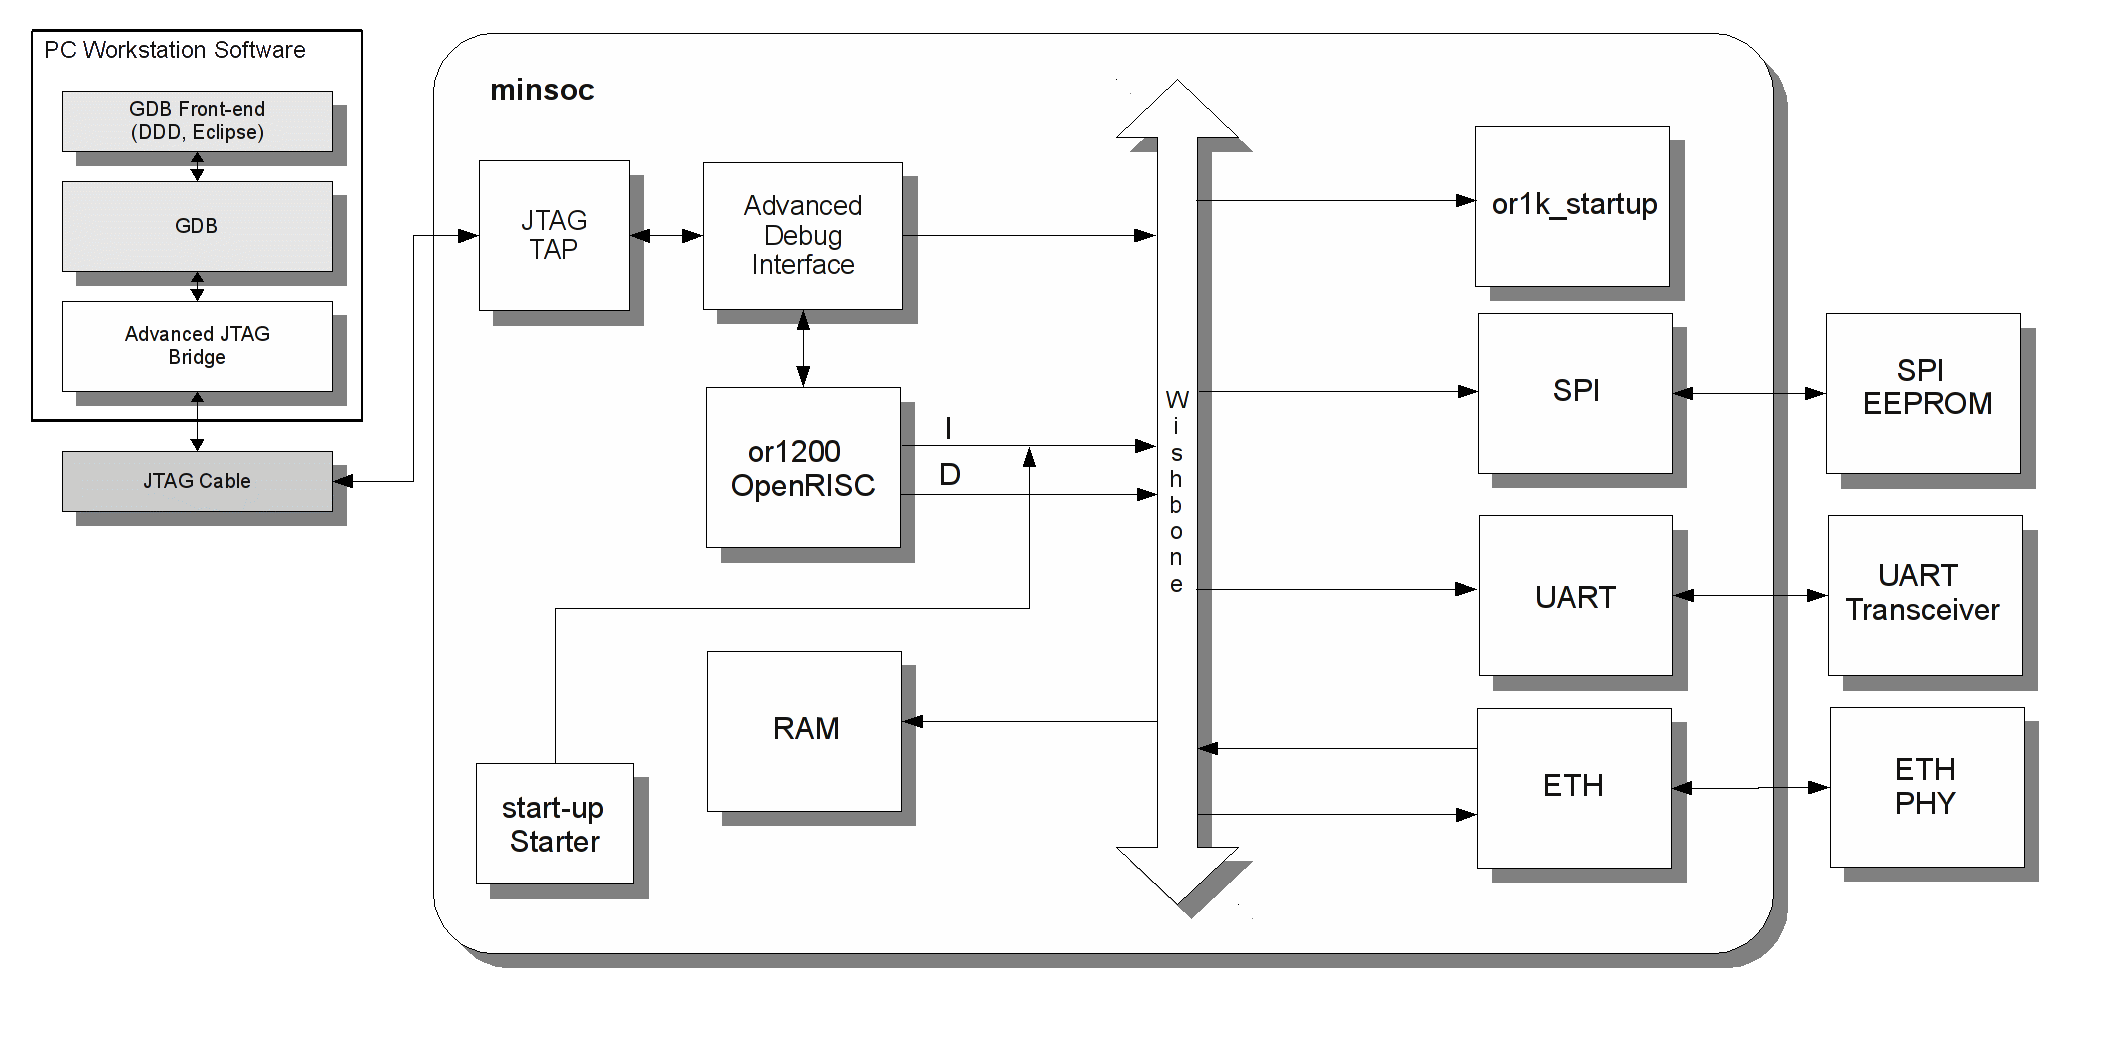
\includegraphics[width=1\textwidth,keepaspectratio=true]{./images/minsoc}
  \caption{Arquitectura MinSoc}
  \label{fig:esquemaminsoc}
 \end{center}
\end{figure}

\begin{itemize}
\item Características:
				\begin{itemize}
				  \item Microprocesador embebido OR1200 OpenRISC 
				  \item memoria redimensionalble
				  \item selección de frecuencia del sistema
				  \item JTAG debug con capacidad para distintos cables
				  \item Posibilitad de arranque automático de un firmware desde una memoria externa SPI
				  \item Modulos de UART y Ethernet 
				  \item Código genérico y especifico de memoria para las FPGA de Xilinx y Altera, adaptación de clock (PLLs y MCMs) y JTAG TAP
				  \item Configuración del sistema en un simple archivo de definición 
				  \item Ejemplos de firmware utilizando UART y Ethernet  
				  \item Incluye testbench para la simulacón de la configuración del sistema. 						
				\end{itemize}

\item Tecnologías probadas que le brindan soporte al proyecot MinSoC:


\begin{itemize}
				  \item Xilinx, Spartan 3E (Spartan3E Starter Kit)
				  \item Xilinx, Spartan 3A (Spartan3A 1800 DSP Kit)
				  \item Xilinx, Virtex 4 (ML405 board)
				  \item Xilinx, Virtex 5 (ML505 board)
				  \item Altera, Cyclone II
				  \item Altera, Cyclone II
				  \item (DE2-70 board)
				  \item Altera, Cyclone III
				  \item Altera, Cyclone IV (Bemicro SDK board) 
				  \item Altera, Stratix II						
				\end{itemize}
\end{itemize}


				\subsection{Proyecto ORPSoC}

				Este proyecto implementa una plataforma para el desarrollo OpenRISC. Está destinado a ser un entorno de desarrollo y verificación de IP cores y
				diseños de SoC. Se trata de un proyecto desarrollado con la colaboración de una de las comunidades mas importantes de hardware de código abierto
				\url{opencores.org}.


El proyecto permite tanto a usuarios nuevos como experimentados realizar diseños con un desarrollo rápido OpenRISC.Está destinado a ser un entorno de desarrollo y verificación de núcleos de propiedad intelectual y diseños SoC.Es un proyecto de desarrollo colaborativo. Como plataforma de desarrollo proporciona un entorno modular y facil de usar, para el desarrollo de código RTL y su posterior simulación y síntesis. Provee un entorno de herramientas para desarrollo de aplicaciones OpenRISC para su simulación y prueba en la placa de desarrollo.

Una visión general sobre el SoC completa y sus conexiones externas es en la  (Figura ~\ref{fig:esquemaorpspc})

\begin{figure}[h!]
 \begin{center}
  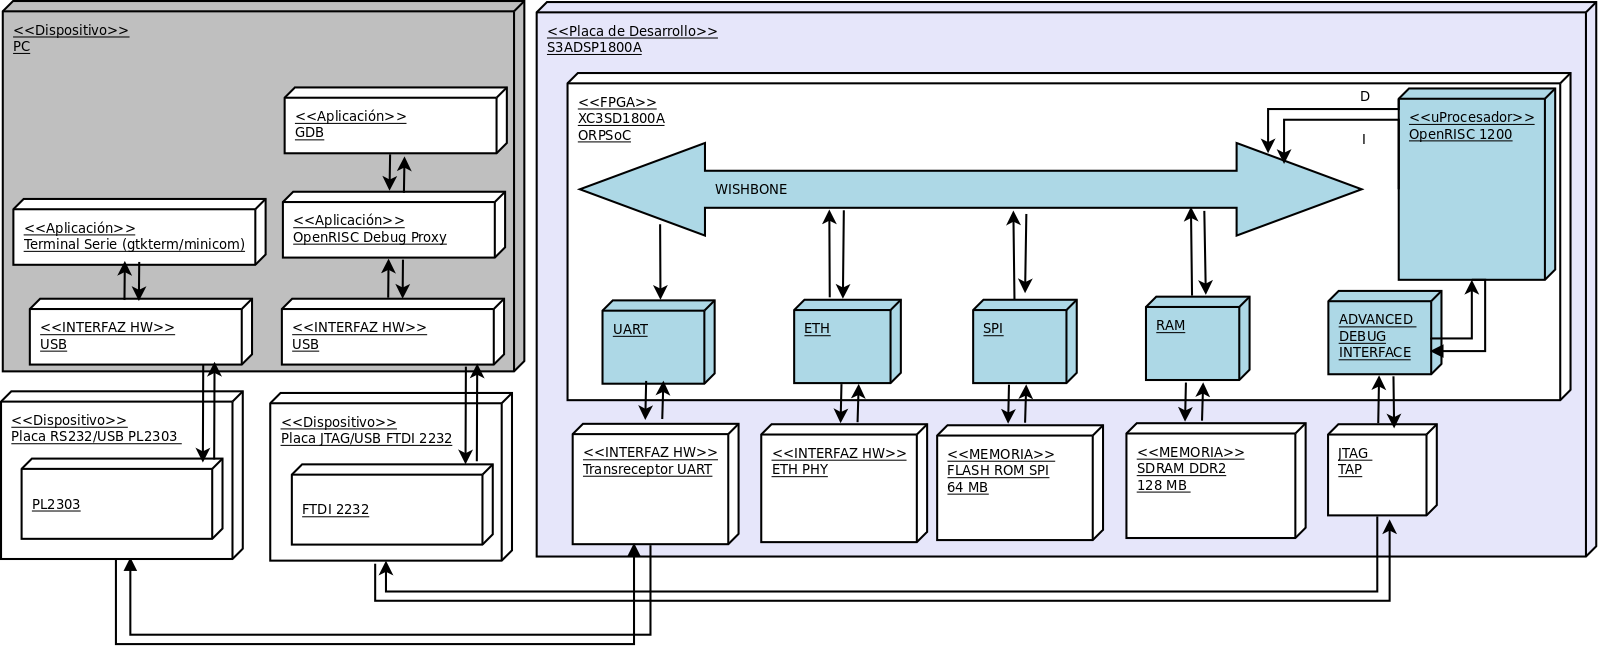
\includegraphics[width=1\textwidth,keepaspectratio=true]{./images/orpsoc}
  \caption{Arquitectura ORPsoc}
  \label{fig:esquemaorpsoc}
 \end{center}
\end{figure}

\begin{itemize}
\item Características:
				\begin{itemize}
				  \item Microprocesador embebido OR1200 OpenRISC 
				  \item memoria redimensionalble
				  \item selección de frecuencia del sistema
				  \item JTAG debug con capacidad para distintos cables
				  \item Posibilitad de arranque automático de un firmware desde una memoria externa SPI
				  \item Modulos de UART y Ethernet 
				  \item Código genérico y especifico de memoria para las FPGA de Xilinx y Altera, adaptación de clock (PLLs y MCMs) y JTAG TAP
				  \item Configuración del sistema en un simple archivo de definición 
				  \item Ejemplos de firmware utilizando UART y Ethernet  
				  \item Incluye testbench para la simulacón de la configuración del sistema. 						
				\end{itemize}

\item Tecnologías probadas que le brindan soporte al proyecot MinSoC:


\begin{itemize}
				%  \item Xilinx, Spartan 3E (Spartan3E Starter Kit)
				  \item Xilinx, Spartan 3A (Spartan3A 1800 DSP Kit)
				  %\item Xilinx, Spartan 6 LX45 (ML405 board)
				  \item Xilinx, Virtex 5 (ML501 board
					% \item Altera, Cyclone II
				  %\item Altera, Cyclone II
				  %\item (DE2-70 board)
				%  \item Altera, Cyclone III
				  \item Altera, Cyclone IV (Terasic DE0 Nano) 
				%  \item Altera, Stratix II						
				\end{itemize}
\end{itemize}

				

\section{Presentación de Placas de Desarrollo}
 
				Los proyectos MinSoC y OrpSoc cuentan actualmente con soporte para diversas placas de desarrollo. 

				\subsection{Xilinx}
				La empresa Xilinx provee kits de desarrollo de diversas características y prestaciones. A continuación se detallan algunas de las alternativas que
				son soportadas por los SoC elegidos.
				\subsubsection{S3ADSP1800A}
				El dispositivo XtremeDSP™ Starter Platform cuenta con una FPGA de la familia Spartan®-3A que permite la evaluación diseños para diferentes
				aplicaciones tales como Prototipado General, Sistemas Embebidos, Video Digital, DSP, Procesamiento de Imagenes, Comunicaciones digitales y
				Coprocesamiento. Esta plataforma provee acceso a las capacidades de la familia de FPGA Spartan®-3A y cuenta con periféricos,conectores e
				interfaces estándar de la industria. Fue diseñada para para ser utilizada con Xilinx System Generator para aplicaciones DSP y las herramientas de
				diseño ISE® o el entorno desarrollado en Linux llamado PetaLinux Software Development Kit (SDK) ambas herramientas provistas por el fabricante. 
				
				%Traducir esto ???
				Las características generales del kit son:
			
				\begin{tabular}{ p{4cm} p{10cm} }
				\rowcolor[gray]{0.8} Caracteristica & Descripción \\		
				\hline FPGA   & XC3SD1800A-4FGG676C Spartan-3A DSP FPGA\\
				\hline Clocks & 125 MHz LVTTL SMT oscillator\\
				\hline        & LVTTL oscillator socket\\
				\hline		  & 25.175 MHz LVTTL SMT oscillator (video clock)\\
				\hline		  & 25 MHz Ethernet clock (accessible to FPGA)\\
				\hline Memory & 128 MB (32M x 32) DDR2 SDRAM\\
				\hline		  & 16Mx8 parallel / BPI configuration flash\\
				\hline 		  & 64 Mb SPI configuration / storage flash (with 4 extra SPI selects)\\
				\hline Interfaces & 10/100/1000 PHY\\
				\hline			  & JTAG programming/configuration port\\
				\hline            & RS232 Port\\
				\hline			  & Low-cost VGA\\
				\hline			  & 4 SPI select lines\\
				\hline Buttons and Switches & 8 user LEDs\\
				\hline  		  & 8-position user DIP switch\\
				\hline            & 4 user push button switches\\
				\hline 			  & Reset push button switch\\
				\hline User I/O and Expansion & Digilent 6-pin header\\
				\hline			 			  & EXP expansion connector\\
				\hline 						  & 30-pin GPIO connector: can be used for System ACE™ Compact Flash daughter card (not included)\\
				\hline Configuration and Debug & JTAG\\
				\hline                         & System ACE module connector\\   
				\end{tabular}
				
				Las implementaciones MinSoC y ORPSoC proveen soporte nativo para los siguientes periféricos:
				
				\begin{itemize}
				  \item Ethernet
				  \item GPIO (Solo ORPSoC)
				  \item DDR2 SDRAM (128MB) (Solo ORPSoC)
				  \item SPI
				  \item UART				
				\end{itemize}
			
				\subsubsection{ML501}
				La ML501 es una plataforma de desarrollo de bajo costo y gran funcionalidad que provee un acceso práctico a los recursos disponibles en el
				dispositivo FPGA Virtex®-5 LX50. Posee interfases y conectores industriales estándar y presenta gran versatilidad para su utilización en
				múltiples aplicaciones como Video, Audio y puertos de comunicación.
				
				Las características generales del kit son:
			
			\begin{tabular}{ p{4cm} p{10cm} }
			\rowcolor[gray]{0.8} Caracteristica & Descripción \\		
			\hline FPGA & XC5VLX50FFG676\\
			\hline Memoria & DDR2 SODIMM (256 MB)\\
			\hline 		   & ZBT SRAM (1 MB)\\
			\hline 		   & Linear Flash (32 MB)\\
			\hline         & System ACE™ CF technology (Compact Flash)\\
			\hline         & Platform Flash\\
			\hline         & SPI Flash\\
			\hline Clocks  & External clocking (2 differential pairs)\\
			\hline Interfaces & USB (2) - host and peripheral\\
			\hline 			  & PS/2 (2) - keyboard, mouse\\
			\hline 			  & RJ-45 - 10/100 Networking\\
			\hline 			  & RS-232 (male) - serial port\\
			\hline 			  & Audio In (2) - line, microphone\\
			\hline 			  & Audio Out (2) - line, amp, SPDIF, piezo speaker\\
			\hline 			  & Video (DVI/VGA) Output\\
			\hline I/O y expansión & Single-ended and differential I/O expansion\\
			\hline GPIO		&  DIP switch (8)\\
			\hline 			&  LEDs (8)\\
			\hline 			&  push buttons (5)\\
			\hline Debug y programación & JTAG programming interface\\
			\hline Medioambiente & EU-RoHS compliant \\
			\end{tabular}
				
				Las implementación ORPSoC fue probada con éxito en esta plataforma y provee soporte para los siguientes periféricos:
				
				\begin{itemize}
				  \item Ethernet
				  \item GPIO
				  \item DDR2 SDRAM (256MB)
				  \item CFI flash (32MB)
				  \item SRAM
				  \item SPI
				  \item UART
				  \item AC97 
				  \item PS/2 				
				\end{itemize}
			
				
				\subsection{Digilent}
				\subsubsection{Atlys}
				La placa de desarrollo Atlys es una plataforma que permite el desarrollo de circuitos digitales y esta soportada por una FPGA Xilinx Spartan 6 LX45. Posee periféricos entre los que se destacan Gbit Ethernet, Video HDMI, Audio, puertos USB y Memoria Ram 128 MB DDR2 que permiten el
				desarrollo de Sistemas Digitales sobre procesadores embebidos como  MicroBlaze de Xilinx. Atlys es compatible con todas las herramientas CAD de
				Xilinx como ChipScope, EDK y WebPack (gratuito) lo que permite completar diseños sin mayor costo. Como alternativa puede utilizarse un entorno de
				desarrollo para Linux llamado PetaLinux Software Development Kit (SDK) provisto por el fabricante de la FPGA.
				
				Las características generales de la plataforma son:
				
				\begin{tabular}{ p{4cm} p{10cm} }
				\rowcolor[gray]{0.8} Caracteristica & Descripción \\		
				\hline FPGA   & Spartan-6 LX45, 324-pin BGA package \\
				\hline 		  &	6,822 slices each containing four 6-input LUTs and eight flip-flops\\
				\hline DSP	  & 58 DSP slices\\
				\hline Clocks & 2.1Mbits of fast block RAM\\
				\hline 		  & 4 clock tiles (8 DCMs \& 4 PLLs)\\
				\hline 		  & 6 phased-locked loops\\
				\hline 		  & 500MHz+ clock speeds\\
				\hline 		  & 100MHz CMOS oscillator\\
				\hline Memoria & 128Mbyte DDR2 16-bit wide data\\
				\hline         & 16Mbyte x4 SPI Flash for configuration \& data storage\\
				\hline GPIO & 8 LEDs \\
				\hline 		& 6 buttons\\
				\hline		& 8 slide switches\\
				\hline Interfaces & 10/100/1000 Ethernet PHY\\
				\hline 			  & On-board USB2 ports for programming \& data transfer\\
				\hline 			  & USB-UART and USB-HID port (for mouse/keyboard)\\
				\hline 			  & Two HDMI video input ports \& two HDMI output ports\\
				\hline			  & AC-97 Codec with line-in, line-out, mic, \& headphone\\
				\hline Energía & Real time power monitors on all power rails\\
				\hline 		   & 20W power supply and USB cable\\
				\hline I/O y Expansión & 48 I/O’s routed to expansion connectors\\
				\end{tabular}
				
				La implementación ORPSoC proveen soporte nativo para los siguientes periféricos:
				
				\begin{itemize}
				  \item AC97
				  \item Ethernet
				  \item GPIO
				  \item PS/2 
				  \item DDR2 SDRAM (128MB)
				  \item SPI
				  \item UART
				  \item VGA
				\end{itemize}				

				\subsection{Terasic}
				\subsubsection{Terasic DE0 Nano}
				La plataforma DE0-Nano posee un tamaño compacto que se ajusta al diseño de circuitos para proyectos portables. Fue diseñada para ser
				utilizada con una implementación simple utilizando como destino una FPGA Cyclone IV de Altera con 22,320 LEs (Elementos Lógicos). Entre sus
				características princpiales se encuentran diversas interfases que incluyen dos puertos de expanxión GPIO, dispositivos de memoria on board SDRAM y
				EEPROM. Las mayores ventajas del DE0-Nano son su reducido tamaño y peso, así como la capacidad de ser reconfigurado sin la necesidad de
				utilización de hardware extra. Los requerimientos de energía para dispositivos portables son cruciales , la DE-0 Nano posee 3 esquemas posibles
				de conexión : un puerto USB mini-AB, conectores de 2 pines para alimentación externa de 5V, y 2 pines de 5V.

				Las características generales de la plataforma son:
				
				\begin{tabular}{ p{4cm} p{10cm} }
				\rowcolor[gray]{0.8} Caracteristica & Descripción \\		
				\hline FPGA   	& Cyclone® IV EP4CE22F17C6N FPGA\\
				\hline 			& 22,320 Logic elements (LEs)\\
				\hline 			& 594 Embedded memory (Kbits)\\
				\hline 			& 66 Embedded 18 x 18 multipliers\\
				\hline			& 4 General-purpose PLLs\\
				\hline 			& 153 Maximum FPGA I/O pins\\ 
				\hline Configuration Status and Set-Up Elements & 	On-board USB-Blaster circuit for programming\\
				\hline											&	FPGA Serial Configuration Device (EPCS)\\
				\hline Expansion Header & 	Two 40-pin Headers (GPIOs) provides 72 I/O pins\\
				\hline 					&	Two 5V power pins, two 3.3V power pins and four ground pins\\
				\hline 					&	One 26-pin header provides 16 digital I/O pins and 8 analog input pins to connect to analog sensors, etc\\ 
				\hline Memory Devices	&	32MB SDRAM\\
				\hline 					&	2Kb I2C EEPROM\\ 
				\hline General User Input/Output 	& 8 green LEDs\\
				\hline 								& 2 debounced push-buttons\\
				\hline 								& 4 dip switches\\ 
				\hline G-Sensor & ADI ADXL345, 3-axis accelerometer with high resolution (13-bit)\\ 
				\hline A/D Converter & NS ADC128S022, 8-Channel, 12-bit A/D Converter\\ 
				\hline					 & 50 ksps to 200 ksps \\
				\hline Clock System & On-board 50MHz clock oscillator\\
				\hline Power Supply & USB Type mini-AB port (5V)\\
				\hline 				& Two DC 5V pins of the GPIO headers (5V)\\
				\hline 				& 2-pin external power header (3.6-5.7V)\\
				\end{tabular}
				
				La implementación ORPSoC proveen soporte nativo para los siguientes periféricos:
				
				\begin{itemize}
				  	\item GPIO
					\item SDRAM (32MB)
					\item UART
					\item SPI FLASH (8MB)
					\item I2C
				\end{itemize}				
				
 		\subsection{Conclusiones de la elección de la Placa de Desarrollo}
 				Se seleccionó entre los items analizados y teniendo en cuenta la disponibilidad de recursos al momento de realizar este trabajo utilizar las
 				placas S3ADSP1800A de Xilinx para soportar los SoC a implementar.
 		
 		\newpage	
 		\section{Presentación de las herramientas de desarrollo} 	 
 				\subsection {Herramientas de Desarrollo de Hardware}
 				Durante el proceso de desarrollo e implementación de hardware mediante lógica programable son necesarias un serie de herramientas que
 				proporcionan diferentes salidas en cada etapa del proceso. En la Figura ~\ref{fig:designflow} se observan las etapas del flujo de diseño y sus
 				respectivas salidas.
 				
 		\begin{figure}[h!]
 		\begin{center}
  		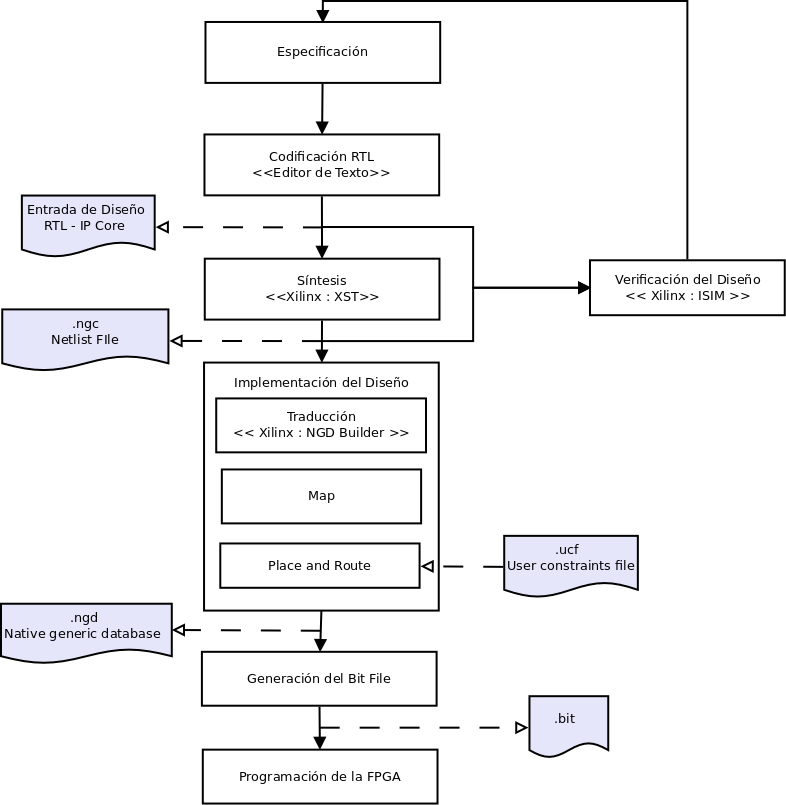
\includegraphics[width=0.7\textwidth,keepaspectratio=true]{./images/designflow}
  		\caption{Flujo de diseño e implementación de hardware con lógica programable}
  		\label{fig:designflow}
 		\end{center}
		\end{figure}
		
				Se analizaron las aplicaciones alternativas para cada etapa, enfatizando la selección de aplicaciones que cumplan con el requerimiento RQX-LC 2
				planteado en la Tabla ~\ref{tab:requsr2}.   
				
				\subsubsection {Codificación RTL - Editores de Texto}
				Existen diversas herramientas de Edición de Texto que poseen características compatibles con el desarrollo de código de descripción de hardware.
				Entre las características más comunes encontramos numeración de líneas, resaltado de código, y predictores. 
				Xilinx provee en su Suite de Desarrollo la posibilidad de confeccionar código directamente desde ISE Project Mananger. Sin embargo,
				existen alternativas Open Source de capacidades comparables tales como emacs o gedit. 
				
				\subsubsection {Síntesis, Implementación del Diseño y Generación del Bit File}
				En estas etapas del proceso de diseño no existen herramientas alternativas con licencias OpenSource que permitan obtener el archivo de
				configuración de la FPGA. Esta restricción obliga a los desarrolladores a utilizar solo las herramientas del fabricante al implentar sus diseños
				en FPGA.
				Para realizar la síntesis, Xilinx, utiliza la aplicación XST que realiza la traducción de la descripción RTL escrita en algún lenguaje de
				descripción de Hardware como Verliog o VHDL en una lista de elementos lógicos y sus conexiones. La siguiente etapa consiste en la implementación 
				del diseño y consta de tres grandes etapas: Translate, Map, Place and Route. Finalizada esta etapa se obtiene el diseño adecuado al modelo de
				fpga seleccionado, sus clocks y sus conexiones de entrada/salida. 
				
				\subsubsection {Programación y Configuración de la FPGA}
				La acción que culmina el proceso de implementación es la descarga del código binario de configuración en la FPGA. El protocolo utilizado para
				realizar esta acción se denomina JTAG (Joint Test Action Group) se encuentra implementado en diversos dispositivos de programación de FPGA y
				microprocesadores. La mayoría de estos dispositivos proveen soporte SPI (Serial Peripheral Interface) que permite el acceso a dispositivos de
				almacenamiento como lo son, por ejemplo, las memorias Flash SPI.
				
				Xilinx provee la aplicación iMPACT con su Suite de Desarrollo ISE. Esta herramienta es compatible con todos los dispositivos fabricados por
				Xilinx y algunos dispositivos incluídos en sus placas de prueba. Durante el desarrollo de este trabajo los autores debieron lidiar con
				problemas de acceso a dispositivos de terceros que conforman la placa de desarrollo S3ADSP1800A que produjeron retrasos significativos en
				realización del proyecto.
 				
 				Alternativamente, existen herramientas Open Source tales como XC3SPROG y UrJTAG , ambos licenciados bajo GPLv2 . La herramienta XC3SPROG
 				posee capacidades comparables al iMPACT y proporciona acceso de diversos disposivitos entre los que se encuentran:
 				\begin{itemize}
 				  \item Dispositivos Xilinx
				  \item Dispositivos Atmel 
				  \item Memorias SPI flash: AT45, AMIC, AMIC-QUAD, M25P, N25Q, S33, W25
 				\end{itemize}
 				 
 				\subsection {Herramientas de Desarrollo de Software}
 			
				Se analizaron las aplicaciones alternativas para cada etapa, enfatizando la selección de aplicaciones que cumplan con el requerimiento RQX-LC 3
				planteado en la Tabla ~\ref{tab:requsr2}.   
				 			
 				\subsubsection {Toolchain para OpenRISC}
 				La comunidad OpenCores realizó una adapatación del Toolchain GNU para generar aplicaciones en C y C++ que se ejecuten en una arquitectura
 				OpenRISC. Así mismo fueron adaptadas las librerias newlib y uClibc conformando una solución completa al diseño y desarrollo de aplicaciones
 				OpenRISC. Existe un entorno de desarrollo gráfico llamado OpenIDEA desarrollado por Dynalith basado en este toolchain. 
				
				El proyecto OpenRISC cuenta con un simulador del repertorio de instrucciones llamado or1ksim que permite la simulación de aplicaciones compiladas
				mediante el toolchain sin necesidad de tener disponible el hardware de prueba durante la etapa de desarrollo de software.
 				
 	

		\section{Presentación de los Sistema Operativo}
 		
			 	\subsection{ecOS}

eCos \cite{Etiqueta35} es un sistema operativo de tiempo real y de código abierto para aplicaciones embebidas, y es desarrollado por eCosCentric, una división de RedHat. Según el autor eCos es el RTOS más popular en la actualidad y ha sido utilizado en varios productos como 
por ejemplo receptores de radio satelital Sirius, módulos Wi-Fi de la consola Sony PlayStation 3 
y routers Netgear, entre otros. 


 eCos viene de "Embedded Configurable Operating System", y según sus creadores puede ser configurado para ejecutarse tanto en dispositivos con memoria muy limitada de tipo SoC (System on a Chip) como en sistemas más complejos que requieren mayores funcionalidades. 
 
El sistema es distribuído sin costo bajo licencia GPL modificada, la cual permite el uso de código propietario en conjunto con eCos. Esto significa que la licencia no requiere que el código desarrollado sobre eCos sea necesariamente de tipo GPL. También existe una versión comercial 
(eCosPro).

Características generales: 
				\begin{itemize}
				  	\item Algoritmo de itineración de tipo Round Robin
					\item Kernel de tipo apropiativo o cooperativo (configurable). Pueden añadirse schedulers 
 adicionales
					\item El Kernel no desactiva las interrupciones
					\item Implementación de mutexes, semáforos binarios y de conteo, variables de condición, 
 casillas de correo, banderas de evento y spinlocks
					\item Memory Allocation: Fixed Block, Variable Block and dynamic heaps. (configurable)
					\item Bibliotecas disponibles ISO C y Math, C++/STL, microITRON y POSIX. 
					\item  Incluye un pequeño stack IP
					\item Sistema de Archivos FAT12/16/32
					\item Incluye un bootloader con opciones de debugging
				\end{itemize}			

Arquitecturas compatibles:

				\begin{itemize}
				\item x86 / i386 / IA-32
				\item x86 Multiprocesamiento simétrico
				\item x86-64
				\item PowerPC Multiprocesamiento simétrico
				\item Alpha
				\item ARM
				\item Intel XScale
				\item M68k
				\item PA-RISC
				\item OpenRISC
				\item CalmRISC
				\item Nios II
			\end{itemize}			

	

			 \subsection{Linux}

El sistema operativo Linux es una implementación de libre distribución UNIX para computadoras personales (PC), servidores, y estaciones de trabajo.Como sistema operativo, Linux es muy eficiente y tiene un excelente diseño.





 
Características generales:

	\begin{itemize}
	\item Licencia de Software: GPL/LGPL
	\item Tipo de núcleo: núcleo monolítico con módulo
	\item Lenguaje de programación del núcleo en c
	\item Soporte de Hilo de ejecución del núcleo: 1:1
	\item Familia de SO tipo UNIX
	\item Comunicación entre procesos y sincronización
	\item Multitarea
	\item Unidad de Gestión de Memoria 
	\item Tecnología de red TCP/IP,IPv6, IPX, PPP, PPPoE, DHCP, bridge, TUN/TAP, ssh, OpenVPN 	
	\item Sistema de archivos NTFS,ext2, MS-DOS, FAT16/32 y otros
	\item Forks: microCLinux	
	
\end{itemize}			

Arquitecturas compatibles:

				\begin{itemize}
				\item x86 / i386 / IA-32
				\item x86 Multiprocesamiento simétrico
				\item Xen
				\item IA-64 	
				\item SPARC32
				\item x86-64
				\item PowerPC
				\item PowerPC Multiprocesamiento simétrico
				\item Alpha
				\item MIPS
				\item ARM
				\item Intel XScale
				\item M68k
				\item PA-RISC
				\item OpenRISC
			\end{itemize}			

%Hardware compatible:

%			\begin{itemize}
%				\item ATA
%				\item SATA
%				\item SCSI
%				\item USB 2.0 	
%				\item USB 1.1
%				\item FireWire
%				\item PCMCIA/PC card
%				\item AGP
%				\item Nvidia official driver IA32
%				\item Nvidia official driver IA64
%				\item Nvidia official driver AMD64
%				\item ATI official driver x86
%				\item ATI official driver x86-64
%				\item Ati r200 free software driver
%				\item Ati r300 free software driver
%				\item Nvidia free software driver
%				\item Audio
%			\end{itemize}
%Interconexión:

%			\begin{itemize}
%				\item Networking supported	
%				\item NE2000/RTL8029
%				\item RTL8139
%				\item Gigabit Ethernet 	
%				\item 10 Gigabit Ethernet
%				\item WLAN
%				\item Bluetooth
%				\item IrDA
%			\end{itemize}

%Tecnologías de red:

%			\begin{itemize}
%				\item Firewall: netfilter/iptables
%				\item TCP/IP	
%				\item IPv6
%				\item IPX 	
%				\item PPP			
%				\item PPPoE
%				\item DHCP
%				\item bridge
%				\item TUN/TAP
%				\item ssh
%				\item OpenVPN
%			\end{itemize}

%Sistemas de archivos compatibles:


%			\begin{itemize}
%				\item FAT16 dosfs, FAT32/vfat	
%				\item NTFS	
%				\item Ext2	
%				\item Ext3	
%				\item XFS	
%				\item ReiserFS	
%				\item UFS	
%				\item UFS2	
%				\item HFS
%				\item HFS+	
%				\item Minixfs	
%				\item BFS	
%				\item ISO 9660	 
%				\item UDF	
%				\item NFS	
%				\item SMBFS	
%				\item Disco RAM/tmpfs	
%				\item procfs	
%				\item Memoria virtual/Swap	
				
%			\end{itemize}


		\subsection{ BusyBox}	
 	
				
			 
BusyBox \cite{Etiqueta36} combina versiones de varias utilidades comunes de UNIX en un sólo ejecutable. Remplaza las utilidades que se suelen encontrar en fileutils GNU, shellutils, etc. Las utilidades en BusyBox tiene menos funciones que GNU, sin embargo, las opciones que incluyen proporcionan la funcionalidades necesarias. BusyBox proporciona un entorno  completo para cualquier sistema pequeño o embebido.

Este conjunto de programas están optimizados de acuerdo a las limitaciones de los recursos disponibles de hardware. También se puede fácilmente incluir o excluir comandos (o características) en tiempo de compilación. Esto hace que sea fácil de personalizar un sistemas embebidos. 

%Para crear un sistema de trabajo, sólo tiene que añadir algunos nodos de dispositivos en / dev, algunos archivos de configuración en / etc, y un núcleo de Linux.

BusyBox es mantenida por Denys Vlasenko, y licenciado bajo la GNU GPL.

%%%%%%%%%%%%%%%%%%%%%%%%%%%

			
 			
 
\end{part}
\begin{part}{Implementación}
\newpage
\chapter{Diseño e Implementación}\label{chap:disenoeimpl}

	\section{Introducción}
	Debido a que se adoptó un modelo de desarrollo en espiral se plantearon una serie de prototipos que incluyen mayor funcionalidad en cada iteración
	del modelo. Inicialmente se planteó un prototipo básico para determinar factibilidad de puesta en funcionamiento de un SoC con microprocesador
	OpenRISC y el desarrollo de aplicaciones que se ejecuten en él. Debido a su funcionalidad reducida y menor consumo de recursos  para su síntesis se
	seleccionó el proyecto MinSoC para el desarrollo del primer prototipo con el cual se evaluaron y documentaron las capacidades del mismo, permitiendo
	valorar este proyecto para aplicaciones donde no se requieren grandes cantidades de memoria y juegan un papel primordial las entradas/salidas junto
	a la capacidad de procesamiento.  
		 
		\subsection{Entorno de ejecución}
		Actualmente OpenRISC es soportado por un conjunto de herramientas de desarrollo(toolchain) de 32 bits ofreciendo soporte para los lenguajes C y C++
		con librerías estáticas. El toolchain se encuentra disponible en dos formas: una para la ejecución de aplicaciones bajo el sistema operativo Linux y
		otra para la ejecución de aplicaciones standalone o bare metal que son aquellas que se ejecutan e interactúan directamente con el hardware sin la
		necesidad de un sistema operativo que proporcione soporte para la utilización de los periféricos.
		
			\subsubsection{Entorno de ejecución Standalone - Bare Metal}
	    	Para la ejecución de aplicaciones Bare Metal el toolchain se basa en la librería newlib que es una implementación estándar utilizada en
	    	sistemas embebidos. 
	    
			\subsubsection{Entorno de ejecución Linux}
			Por otro lado, para el uso de aplicaciones bajo el sistema operativo Linux el toolchain puede ser compilado en base a la librería uClibc que es la
			opción para sistemas embebidos de la librería glibc utilizada en los sistemas estándar.

		\subsection{Matriz de riesgo}
En cada prototipo se tienen en cuenta los posibles riesgos ya mencionadas y se amplían según la nueva visión del sistema.
		
		\subsection{Criterio para la realización de testing}%%corregir esto
		El testing desarrollado apunta a verificar el cumplimiento de los requerimientos individualmente e incrementalmente. Se pretende utilizar las
		aplicaciones de prueba provistas y desarrollar algunas que verfiquen los requerimientos de compilación, depuración y ejecución de aplicaciones para
		OpenRISC. 
		Los testing sirven para poder detectar la presencia de errores, pero aún si un testing no arroja resultados erróneos, esto no nos garantiza el
		correcto funcionamiento del sistema. El tipo de testing realizado es de verificación. La verificación es el proceso de evaluación de un sistema o
		componente para determinar si el producto cumple con lo que se ha diseñado, es decir, si cada fase de desarrollo dada cumple con los requisitos
		impuestos al inicio de dicha fase.

\newpage
\chapter{Prototipo Uno : Implementación del SoC MinSoC en FPGA}

	\section{Introducción}
		
	En este primer prototipo se implementó el proyecto MinSoC en la placa de desarrollo S3ADSP1800A con el fin de verificar el funcionamiento del procesador y sus periféricos. Para lograr este objetivo se requiere de la instalación y puesta en funcionamiento de las herramientas de síntensis, place \& route(PAR) y programación de la FPGA Spartan 3A. 

	\section{Requerimientos del prototipo}
		\begin{table}[h]
		\centering
		\begin{tabular}{ p{2.5cm} p{8cm} p{3cm} }
		\hline 
		\rowcolor[gray]{0.8} N\textordmasculine Req & Descripción\\
		\hline 
		RQX-PA 1 & El prototipo debe implementar un SoC MinSoC en la placa desarrollo S3ADSP1800A\\ 
		\hline 
		RQX-PA 2 & El prototipo debe garantizar el correcto funcionamiento de todos los periféricos conectados al SoC mediante el bus Wishbone\\ 
		\hline 
		RQX-PA 3 & El prototipo debe interactuar correctamente con las interfaces hardware soportadas de la placa de desarrollo S3ADSP1800A\\ 
		\hline
		RQX-PA 4 & El prototipo debe ser capaz de ejecutar programas con capacidad de depuración generados mediante compilación
		cruzada en una arquitectura x86 y/o x86\_64 para la arquitectura OpenRISC\\
		\hline
		RQX-PA 5 & Se debe lograr depurar paso a paso y mediante break points las aplicaciones desarrolladas\\
		\hline		
		\end{tabular}
		\end{table}

\newpage
	
	\section{Matriz de Riesgo para el Prototipo Uno}

		\begin{table}[h!]
		\centering
		\begin{tabular}{ p{2.5cm} p{9cm} p{2cm} p{2cm} }
		\hline 
		\rowcolor[gray]{0.8} N\textordmasculine Req Asociados& Riegos Asociados & Severidad  & Ocurrencia \\
		\hline
		RQX-PA 1& EL código RTL disponible en la web tenga fallas reconocidas durante el proceso de síntesis & Crítica       & Probable \\
		\hline
				& Vencimiento de licencias de las herramientas privativas para el proceso de síntesis  & Menor  & Ocasional\\	 
		\hline
				& Falta de documentación de apoyo para la implentación
del Soc & Crítico & Ocasional\\	 
		\hline

		RQX-PA 2,RQX-PA 3 & Imposibilidad de acceso a alguno de los periféricos de la placa de desarrollo &  Catastrófico  & Probable\\
		\hline
		& Soporte de acceso a periféricos inexistente o con presencia
de bugs & Crítica  & Ocasional\\	 
		\hline
		RQX-PA 4& Compilación cruzada realizada con compiladores obsoletos & Severo  &  Ocasional\\ 
		\hline
		&Problemas en la compilación e instalación de las herramientas de desarrollo de software  & Severo  &  Ocasional\\ 
		\hline
		RQX-PA 5& Problemas con el driver provisto por el fabricante del  dispositivo programador JTAG -USB & Severo&  Ocasional\\
		\hline
		\end{tabular}
		\caption{Tabla de Riegos vs. Requerimientos}
		%\label{tab:riegos}
		\end{table}



		\begin{table}[h!]
		\centering
		\begin{tabular}{ p{4cm} p{4cm} p{4cm} p{3cm} }
		\hline 
		\rowcolor[gray]{0.8} Riesgo & Consecuencia & Estrategia preventiva & Estrategia de contingencia\\
		\hline
		EL código RTL disponible en la web tiene fallas reconocidas durante el proceso de síntesis.&Retraso en los tiempos de implementación.& Análisis previo de guías de resolución de problemas y preguntas frecuentes & Revisión de código y consulta a los desarrolladores \\
		\hline
		Vencimiento de licencias de las herramientas privativas para el proceso de síntesis & Imposibilidad de ejecución de las herramientas requeridas & Verificación previa de los vencimientos de las licencias & Renovación de licencia \\	 
		\hline
		Falta de documentación de apoyo para la implentación
del Soc& Perdida de tiempo en realizar la implementación
del SoC & Revisión previa de la documentación existente para la elección del
SoC & Dedicación de mayor tiempo para la implementación\\ 
		\hline
		 Imposibilidad de acceso a alguno de los periféricos de la placa de desarrollo & Imposibilitad de acceso a los periféricos del kit &Verificación previa de los recursos utilizados por el SoC a implementar & Depuración del codigo RTL del proyecto\\		
		\hline
		Problemas con el driver provisto por el fabricante del  dispositivo programador JTAG -USB  & Imposibilidad de configuración de la FPGA y depuración de aplicaciones &Análisis previo de los driver de los dispositivos a utilizar &  Utilización de dispositivos alternativos.\\		
		\hline
		\end{tabular}
		\caption{Planificación de riesgos}
		%\label{tab:planificación}
		\end{table}



		\newpage
		\section{Descripción de la Estructura del Prototipo Uno}
			

		La Figura ~\ref{fig:minsoc} muestra un diagrama de despliegue del prototipo planteado. Se utiliza un estación de trabajo corriendo las herramientas de compilación (GCC) y depuración (GDB) en sus versiones de compilación cruzada para arquitecturas destino OpenRISC. Se requiere de un
		servidor que proporcione un puerto para la depuración con GDB, acción realizada por la aplicación Advanced JTAG Bridge que provee la interfase de comunicación entre el TAP JTAG conectado al SoC a través el cable JTAG y la estación de trabajo.
		
		\begin{figure}[!h]
 		\begin{center}
  		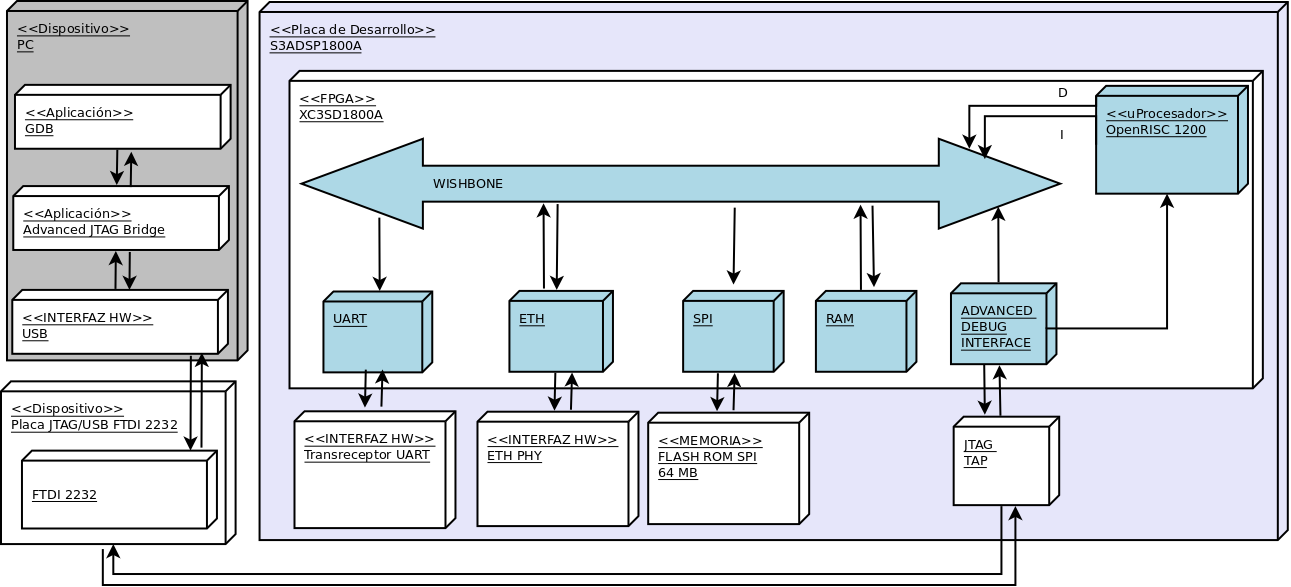
\includegraphics[width=1\textwidth,keepaspectratio=true]{./images/proto1}
  		\caption{Diagrama de despliegue Prototipo Uno}
  		\label{fig:minsoc}
 		\end{center}
		\end{figure}
		
		El módulo Advanced Debug Interface proporciona soporte para la depuración via JTAG, está conectado directamente al microprocesador y a su vez al bus
		general Wishbone donde se conectan el resto de los periféricos. Se conectan al sistema mediante el bus antes mencionado: un modulo	de RAM
		sintetizado, un módulo de arranque (startup), un módulo SPI que interactúa con la memoria flash on board de la placa S3ADSP1800A , un módulo UART y
		un módulo ETHERNET. El sistema inyecta un pequeño código de arranque directamente al bus de instrucciones al iniciar o luego de un reset. 

\newpage
			
		\section{Implementación}

La implementación se realiza normalmente en cinco pasos básicos: 
\begin {itemize}
\item Descarga del script de instalación.
\item Ejecución del script de instalación.
\item Configuración de la placa especifica para la síntesis.
\item Generación del flujo de bits.
\item Programación de la FPGA Spartan 3a.
 \end {itemize}
 Consulte la Guía de MinSoc en el Anexo 1 para la realización pasos a seguir en la implementación sobre la placa de desarrollo  S3ADSP1800A.
		
		%%%%%%%\subsection{Diagrama de Secuencia}
		%\subsection{Selección y Desarrollo de aplicaciones de prueba}
\newpage
		\section{Testing}

% Escribir sobre el testing del proto uno

\begin{table}[h!]
		\centering
		\begin{tabular}{ p{5cm} p{10cm}  }
		\hline 
	    \rowcolor[gray]{0.8}  Caso de Prueba&  Interactuar correctamente con las interfaz hardware UART\\
		\hline 
		Código de Requerimiento & RQX-PA 3\\ 
		\hline 
		Requerimiento  &  El prototipo debe interactuar correctamente con las interfaces hardware soportadas de la placa de desarrollo S3ADSP1800A\\ 
		\hline 
		Código de Testing & T001\\ 
		\hline
		Propósito & Comprobación del correcto funcionamiento de el componente UART \\
		\hline
		Realizado Por & Lovaisa Michelini, Valeria \\
		\hline	
		Entorno de Ejecución & Bare Metal \\
		\hline
		Precondiciones &  \begin {itemize}
							\item Instanciación en la FPGA del SoC.
							\item Ejecución de una terminal serie en la PC
							\item Comunicación establecida entre la placa de desarrollo y la PC
							\end {itemize}\\
		\hline
		Secuencia de Ejecución & Ejecutación de la aplicación de prueba uart.or32  \\
		\hline
		Postcondiciones & MinSoc corriendo sobre FPGA, lo que se manifiesta en la impresión de pantalla de la terminar remota en la PC\\
		\hline
 \multicolumn{2}{>{\columncolor[gray]{.8}}c}{Resultados}\\
		\hline
		Resultados Esperados & Poder observar por la terminal serial una cadena de string.\\
		\hline	
		Resultados Obtenidos & Al ejecutarse la aplicación de prueba del uart se pudo observar la cadena de string esperada "HELLO WORLD" \\
		\hline
		\end{tabular}
		\end{table}

\newpage
\begin{table}[h!]
		\centering
		\begin{tabular}{ p{5cm} p{10cm}  }
		\hline 
	\rowcolor[gray]{0.8}  Caso de Prueba&  Interactuar correctamente con las interfaces hardware de Ethernet\\
		\hline 
		Código de Requerimiento & RQX-PA 3\\ 
		\hline 
		Requerimiento  &  El prototipo debe Interactuar correctamente con las interfaces hardware soportadas de la placa de desarrollo S3ADSP1800A\\ 
		\hline 
		Código de Testing & T002\\ 
		\hline
		Propósito &  El envío de paquetes de Ethernet mediante broadcast desde el SoC  \\
		\hline
		Realizado Por & Gomez, Pablo \\
		\hline	
		Entorno de Ejecución & Bare Metal \\
		\hline
		Precondiciones & \begin {itemize}
							\item Instanciación en la FPGA del SoC.
							\item Ejecución de una terminal serie en la PC
							\item Ejecución de una aplicación snifer en la PC
							\item Comunicación establecida entre la placa de desarrollo y la PC
							\end {itemize} \\
		\hline
		Secuencia de Ejecución &  Ejecutación de la aplicación de prueba eth.or32\\
		\hline
		Postcondiciones &  MinSoc corriendo sobre FPGA, lo que se manifiesta en la impresión de pantalla de la terminar serie en la PC y en los paquetes captados por la aplicación wireshark \\
		\hline
 		\multicolumn{2}{>{\columncolor[gray]{.8}}c}{Resultados}\\
		\hline
		Resultados Esperados & Poder observar por la terminal serial una cadena de string indicando el inicio del envío de paquetes Ethernet y verificar la llegada de los mismos por medio de una aplicación sniffer \\
		\hline	
		Resultados Obtenidos & Al ejecutarse un programa de prueba pudo observarse la cadena de string "HELLO WORLD " y observar 0xFF02B4050 en los paquetes catados por la aplicación wireshark" \\
		\hline
		\end{tabular}
		\end{table}

%%%%%%%%%%%%%%%%%%%%%%%%%%%%%%%%%%%%%%%%%
\newpage
\begin{table}[h!]
		\centering
		\begin{tabular}{ p{5cm} p{10cm}  }
		\hline 
		\rowcolor[gray]{0.8}  Caso de Prueba& Ejecución de la aplicación multiplicadora de matrices binarias generadas mediante una Secuencia binaria pseudo aleatoria (PRBS) \\
		\hline 
		Código de Requerimiento & RQX-PA 4\\ 
		\hline 
		Requerimiento  &  El prototipo debe ser capaz de ejecutar programas con capacidad de depuración, generados mediante compilación cruzada en una arquitectura x86 y/o x86\_64 para arquitectura la OpenRISC\\ 
		\hline 
		Código de Testing & T003\\ 
		\hline
		Propósito &  Compilación y Ejecución de un  programa sencillo en c.Verificación de la capacidad de procesamiento del sistema mediante la realización de los productos con matrices cuadradas incrementando su tamaño iteración a iteración.  
\\
		\hline
		Realizado Por & Gomez, Pablo \\
		\hline	
		Entorno de Ejecución & Bare Metal \\
		\hline
		Precondiciones &\begin {itemize}
							\item Instanciación en la FPGA del SoC.
							\item Ejecución de una terminal serie en la PC
							\item Descarga e instalación del complicador cruzado 
							\item Comunicación establecida entre la placa de desarrollo y la PC
							\end {itemize}
 \\
		\hline
		Secuencia de Ejecución & Ejecución de la aplicación multiplicadora de matrices mult mat.or32 \\
		\hline
		Postcondiciones & Aplicación corriendo sobre el MinSoc instanciado en la FPGA, lo que se manifiesta en la impresión de pantalla de los tiempos de resolución del conjunto de matrices cuadradas multiplicadas en la terminar serie en la PC \\
		\hline
 		\multicolumn{2}{>{\columncolor[gray]{.8}}c}{Resultados}\\
		\hline
		Resultados Esperados & Poder ver la ejecución correcta de un programa de prueba desarrollado \\
		\hline	
		Resultados Obtenidos & Al ser ejecutado se observaron los resultados mostrados en el Bloque ~\ref{lst:salidamult}   \\
		\hline
		\end{tabular}
		\end{table}

\newpage
\begin{lstlisting}[caption={Salida de la terminal serie durante la ejecución del programa multmat.or32},label={lst:salidamult}]
Tick de ejecucion setup tick :0x00000029 En us = 0x00000802
0x00000001
Tick de ejecucion seteo de variables :0x000177a6
Tick de ejecucion de la multiplicacion :0x00000316
0x00000002
Tick de ejecucion seteo de variables :0x0001be62
Tick de ejecucion de la multiplicacion :0x00000fc8
0x00000003
Tick de ejecucion seteo de variables :0x0002344b
Tick de ejecucion de la multiplicacion :0x00002e98
0x00000004
Tick de ejecucion seteo de variables :0x0002d952
Tick de ejecucion de la multiplicacion :0x000067a8
0x00000005
Tick de ejecucion seteo de variables :0x0003ad86
Tick de ejecucion de la multiplicacion :0x0000c31a
0x00000006
Tick de ejecucion seteo de variables :0x0004b0e7
Tick de ejecucion de la multiplicacion :0x00014910
0x00000007
Tick de ejecucion seteo de variables :0x0005e366
Tick de ejecucion de la multiplicacion :0x000201ac
0x00000008
Tick de ejecucion seteo de variables :0x00074512
Tick de ejecucion de la multiplicacion :0x0002f510
0x00000009
Tick de ejecucion seteo de variables :0x0008d5eb
Tick de ejecucion de la multiplicacion :0x00042b5e
0x0000000a
Tick de ejecucion seteo de variables :0x000a95e7
Tick de ejecucion de la multiplicacion :0x0005acb8
0x0000000b
Tick de ejecucion seteo de variables :0x000c850b
Tick de ejecucion de la multiplicacion :0x00078140
0x0000000c
Tick de ejecucion seteo de variables :0x000ea357
Tick de ejecucion de la multiplicacion :0x0009b118
0x0000000d
Tick de ejecucion seteo de variables :0x0010f0d0
Tick de ejecucion de la multiplicacion :0x000c4462
0x0000000e
Tick de ejecucion seteo de variables :0x00136d62
Tick de ejecucion de la multiplicacion :0x000f4340
0x0000000f
Tick de ejecucion seteo de variables :0x00161921
Tick de ejecucion de la multiplicacion :0x0012b5d4
Fin del programa

\end{lstlisting}

%%%%%%

\newpage
\begin{table}[h!]
		\centering
		\begin{tabular}{ p{5cm} p{10cm}  }
		\hline 
		\rowcolor[gray]{0.8}  Caso de Prueba&  Se debe lograr depurar paso a paso y mediante break points las aplicaciones desarrolladas\\
		\hline 
		Código de Requerimiento & RQX-PA 5\\ 
		\hline 
		Requerimiento  &  Se debe lograr depurar paso a paso y mediante break points las aplicaciones desarrolladas\\ 
		\hline 
		Código de Testing & T005\\ 
		\hline
		Propósito &   Compilación en modio debug y Ejecución de un programa  en c mediante GDB.Verificar si la cadena de debug está funcionando.  \\
		\hline
		Realizado Por & Gomez, Pablo \\
		\hline	
		Entorno de Ejecución & Bare Metal \\
		\hline
		Precondiciones & \begin {itemize}
							\item Instanciación en la FPGA del SoC.
							\item Ejecución de una terminal serie en la PC
							\item Aplicación compilada con flag de depuración. 
							\item Comunicación establecida entre la placa de desarrollo y la PC
							\end {itemize}
\\
		\hline
		Secuencia de Ejecución &  Ejecución de la aplicación multiplicadora de matrices multmat.or32\\
		
		\hline
		Postcondiciones & Aplicación corriendo en modo debug sobre el MinSoc instanciado en la FPGA, lo que se manifiesta en la detención de la ejecución en cada punto de parada.\\
		\hline
 		\multicolumn{2}{>{\columncolor[gray]{.8}}c}{Resultados}\\
		\hline
		Resultados Esperados & Poder observar paso a paso le ejecución del programa. \\
		\hline	
		Resultados Obtenidos & El programa puede verse a través de la terminal serie detenido en cada punto de parada. \\
		\hline
		\end{tabular}
		\end{table}


		\section{Conclusión}
Este prototipo fue de vital importancia permitiendo mostrar que es posible instanciar sobre el kit de desarrollo disponible un system on de chip básico open source en una FPGA Spartan 3A.
La mayor cantidad de tiempo fue para la  determinación de las herramientas de desarrollo necesarias para el hardware disponible, ya que la documentación sobre el tema era insuficiente o nula. Sin embargo una vez que se pudo logrado encontrar las herramientas adecuadas y  la corrección de error en el código RTL fue mucho más sencillo la implementación del prototipo.
		
\newpage		
\chapter{Prototipo Dos : Implementación del SoC ORPSoC en FPGA}
		\section{Introducción}
		Para el prototipo dos se planteó la implementación de un sistema ORPSoC que dispone de mayor cantidad de periféricos que el MinSoC entre ellos un
		módulo que permite manejar las memorias RAM DDR2 incluídas en la placa de desarrollo S3ADSP1800A. Se verificó inicialmente si la herramientas
		utilizadas en el prototipo uno proporcionaban los mismos resultados en este prototipo y luego se ejecutaron las pruebas de funcionamiento del
		procesador, los periféricos y las herramientas de desarrollo y depuración. 
		
		\section{Requerimientos del prototipo}
		\begin{table}[h!]
		\centering
		\begin{tabular}{ p{2.5cm} p{8cm} p{3cm} }
		\hline 
		\rowcolor[gray]{0.8} N\textordmasculine Req & Descripción\\
		\hline 
		RQX-PB 1 & El prototipo debe implementar un SoC ORPSoC en la placa desarrollo S3ADSP1800A\\ 
		\hline 
		RQX-PB 2 & El prototipo debe garantizar el correcto funcionamiento de todos los periféricos conectados al SoC mediante el bus Wishbone\\ 
		\hline 
		RQX-PB 3 & El prototipo debe interactuar correctamente con las interfaces hardware soportadas de la placa de desarrollo S3ADSP1800A\\ 
		\hline
		RQX-PB 4 & Se debe garantizar el acceso a las memorias RAM DDR2 de la plataforma S3ADSP1800A\\
		\hline
		RQX-PB 5 & El prototipo debe ser capaz de ejecutar programas con capacidad de depuración generados mediante compilación
		cruzada en una arquitectura x86 y/o x86\_64 para arquitectura la OpenRISC\\
		\hline
		RQX-PB 6 & Se debe lograr depurar paso a paso y mediante break points las aplicaciones desarrolladas\\
		\hline
		RQX-PB 7 & El prototipo debe ser evaluado mediante el benchmark CoreMark para el posterior análisis de las capacidades del SoC\\
		\hline		
		\end{tabular}
		\end{table}

\newpage
		\section{Matriz de Riesgo para el Prototipo Dos} 

		\begin{table}[h!]
		\centering
		\begin{tabular}{ p{2.5cm} p{9cm} p{2cm} p{2cm} }
		\hline 
		\rowcolor[gray]{0.8} N\textordmasculine Req Asociados& Riegos Asociados & Severidad  & Ocurrencia \\
		\hline
		RQX-PB 1& EL código RTL disponible en la web tenga fallas reconocidas durante el proceso de síntesis & Crítica       & Probable \\
		\hline				
				& Falta de documentación de apoyo para la implentación
del Soc & Crítico & Ocasional\\	 
		\hline
		RQX-PB 2,RQX-PB 3,RQX-PA 4 & Imposibilidad de acceso a SDRAM DDR2 de lo kit& Catastrófico & Probable\\
		\hline
		RQX-PB 5&Problemas en la compilación e instalación de las herramientas de desarrollo de software  & Severo  &  Ocasional\\ 
		\hline
		RQX-PB 6& Problemas de compactibilidad con el modulo de debug del proyecto ORPSoC  & Crítico&  Ocasional\\
		\hline
		RQX-PB 7 & Problemas con el compilador para la generación del binario del benchmark CoreMark  & Crítico&  Ocasional\\
		\hline
		\end{tabular}
		\caption{Tabla de Riegos vs. Requerimientos}
		%\label{tab:riegos}
		\end{table}

\newpage

 		\begin{table}[h!]
		\centering
		\begin{tabular}{ p{4cm} p{4cm} p{4cm} p{3cm} }
		\hline 
		\rowcolor[gray]{0.8} Riesgo & Consecuencia & Estrategia preventiva & Estrategia de contingencia\\
		\hline
		EL código RTL disponible en la web tiene fallas reconocidas durante el proceso de síntesis.&Retraso en los tiempos de implementación.& Análisis previo de guías de resolución de problemas y preguntas frecuentes & Revisión de código y consulta a los desarrolladores \\		 
		\hline
		Falta de documentación de apoyo para la implentación
del Soc& Perdida de tiempo en realizar la implementación
del SoC & Revisión previa de la documentación existente para la elección del
SoC & Dedicación de mayor tiempo para la implementación\\ 
		\hline
		 Imposibilidad de acceso a SDRAM DDR2 de lo kit & Falta de capacidad para la ejecución de aplicaciones & Analisis previa de guia de resolución de problemas y documentación del core RAM & Depuración del codigo RTL del proyecto\\
		\hline
		Problemas en la compilación e instalación de las herramientas de desarrollo de software & Imposibilidad de desarrollo de aplicaciones que se ejecuten en el proyecto ORPSoC & Verificar la posibilidad de ejecución de las herramientas en diferentes SO & Utilización de las herramientas en alguno de los SO compatibles\\			
		\hline
		Problemas de compatibilidad con el modulo de debug del proyecto OrpSoC con el programador JTAG-USB & Imposibilidad depuración de aplicaciones &Análisis de la documentación del proyecto& Utilización de otros  dispositivos compatibles.\\		
		\hline
		Problemas con el compilador para la generación del binario del benchmark CoreMark & Imposibilidad de medir el rendimiento de la unidade centrales de procesamiento (CPU) & Verificar la posibilidad de ejecución de las herramientas en diferentes SO & Utilización de métodos alternativos para medir el redimiento en sistemas embebidos.\\
		\hline
		\end{tabular}
		\caption{Planificación de riesgos}
		%\label{tab:planificación}
		\end{table}


\newpage
		\section{Descripción de la Estructura del Prototipo Dos}
		La Figura ~\ref{fig:orpsoc} muestra un esquema de la arquitectura planteada en el prototipo. Al igual que en el prototipo uno se utiliza un estación
		de trabajo corriendo las herramientas de compilación (GCC) y depuración (GDB) en sus versiones de compilación cruzada. Se requiere de un servidor
		que proporcione un puerto para la depuración con GDB y a diferencia del prototipo uno este servicio lo proporciona la aplicación OpenRISC Debug
		Proxy.
		
		\begin{figure}[!h]
 		\begin{center}
  		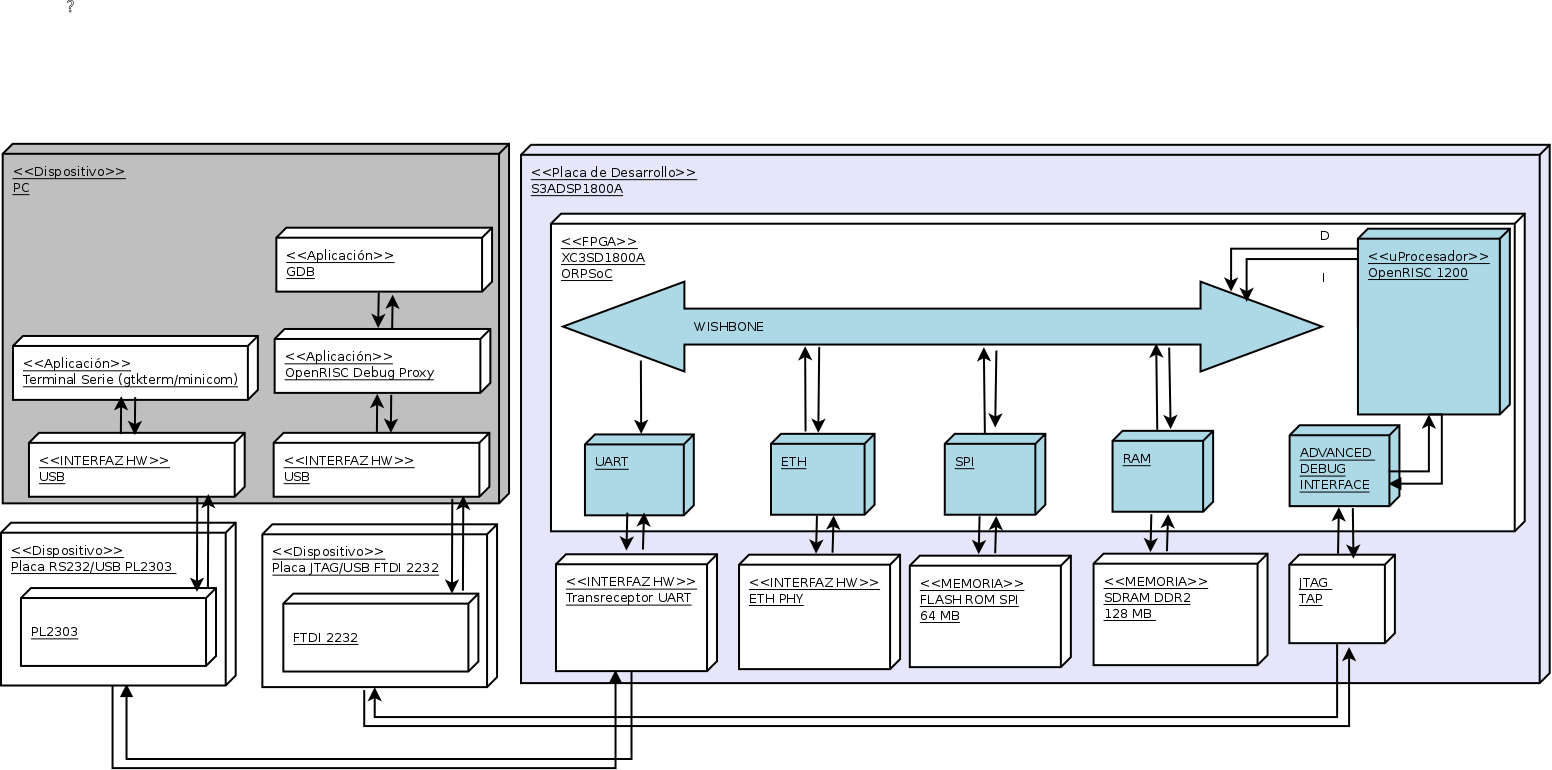
\includegraphics[width=1\textwidth,keepaspectratio=true]{./images/ORPSoCdia}
  		\caption{Arquitectura Prototipo Dos}
  		\label{fig:orpsoc} 
 		\end{center}
		\end{figure}
	
		\section{Implementación}

		La implementación se realiza normalmente en cinco pasos básicos: 
		\begin {itemize}
		\item Descarga del script de instalación.
		\item Ejecución del script de instalación.
		\item Configuración de la placa especifica para la síntesis.
		\item Generación del flujo de bits.
		\item Programación de la FPGA Spartan 3a.
 		\end {itemize}
 
 Puede consultarse la Guía de ORPSoC en el Anexo ~\ref{app:apendice2} para una comprensión más profunda de los pasos a seguir en la implementación
 sobre la placa de desarrollo S3ADSP1800A.

El módulo de Debug proporciona soporte para la depuración via JTAG. Se conectan al sistema mediante un Bus Wishbone: un modulo de RAM que provee acceso a las memorias SDRAM on board de la placa S3ADSP1800A, un módulo SPI que interactúa con la memoria flash on board de la placa antes mencionada, un módulo UART y un módulo ETHERNET. 
		


%%%%%%%%%%%%%%%%%%%%%%%%%%%%TESTING DOS
\newpage
		\section{Testing}

		\begin{table}[h!]
		\centering
		\begin{tabular}{ p{5cm} p{10cm}  }
		\hline 
		\rowcolor[gray]{0.8}  Caso de Prueba&  Interactuar correctamente con las interfaces hardware de Ethernet\\
		\hline 
		Código de Requerimiento & RQX-PB 2 , RQX-PB 3\\ 
		\hline 
		Requerimiento  &El prototipo debe garantizar el correcto funcionamiento de todos los periféricos conectados al SoC mediante el bus Wishbone\\ 
						&  El prototipo debe Interactuar correctamente con las interfaces hardware soportadas de la placa de desarrollo S3ADSP1800A\\
		\hline 
		Código de Testing & T008\\ 
		\hline
		Propósito &  El envío de paquetes echo del protocolo ICMP desde el SoC  \\
		\hline
		Realizado Por & Gomez, Pablo \\
		\hline	
		Entorno de Ejecución & Bare Metal \\
		\hline
		Precondiciones & \begin {itemize}
							\item Instanciación en la FPGA del SoC.
							\item Ejecución de una terminal serie en la PC
							\item Ejecución de una aplicación snifer en la PC
							\item Comunicación establecida entre la placa de desarrollo y la PC
							\item Herramientas de compilación cruzada funcionando correctamente
							\item Programas de prueba compilados correctamente
							\end {itemize} \\
		\hline
		Secuencia de Ejecución &  Ejecutación de la aplicación de prueba ethmac-ping.or32\\
		\hline
		Postcondiciones &  El programa de prueba ejecutándose sobre la RAM de la plataforma, lo que se manifiesta en la impresión de pantalla de la terminar serie en la PC y en los paquetes captados por la aplicación wireshark \\
		\hline
 		\multicolumn{2}{>{\columncolor[gray]{.8}}c}{Resultados}\\
		\hline
		Resultados Esperados & Poder observar por la terminal serial una cadena de string indicando el inicio del envío de paquetes ICMP y verificar la llegada de los mismos por medio de una aplicación ICMP \\
		\hline	
		Resultados Obtenidos & Al ejecutarse el programa de prueba pudo observarse la cadena mostrada en la Referencia ~\ref{lst:reseth}\\
		\hline
		\end{tabular}
		\end{table}


\begin{lstlisting}[frame=single,caption={Salida de la terminal serie durante la ejecución del programa ethmac-ping.or32},label={lst:reseth}]
eth ping program
board IP : 192.168.1.2
\end{lstlisting}


\newpage


		\begin{table}[h!]
		\centering
		\begin{tabular}{ p{5cm} p{10cm}  }
		\hline 
	    \rowcolor[gray]{0.8}  Caso de Prueba&Interactuar correctamente con la memoria RAM. \\
		\hline 
		Código de Requerimiento & RQX-PB 4 \\ 
		\hline 
		Requerimiento  &  Se debe garantizar el acceso a las memorias RAM DDR2 de la plataforma S3ADSP1800A\\ 	

		\hline 
		Código de Testing & T007\\ 
		\hline
		Propósito & Comprobación del correcto funcionamiento del módulo de RAM implementado en el SoC\\
		\hline
		Realizado Por & Lovaisa Michelini, Valeria \\
		\hline	
		Entorno de Ejecución & Bare Metal \\
		\hline
		Precondiciones &  \begin {itemize}
							\item Instanciación del SoC en la FPGA.
							\item Ejecución de una terminal serie en la PC
							\item Comunicación establecida entre la placa de desarrollo y la PC
							\item Herramientas de compilación cruzada funcionando correctamente
							\item Programas de prueba compilados correctamente
							\end {itemize}\\
		\hline
		Secuencia de Ejecución & Ejecutación de la aplicación de prueba sdra-row.or32 \\
		\hline
		Postcondiciones & ORPSoC corriendo sobre FPGA, y la aplicación ejecutándose sobre la memoria RAM lo que se manifiesta en la impresión de pantalla de la terminar remota en la PC\\
		\hline
 		\multicolumn{2}{>{\columncolor[gray]{.8}}c}{Resultados}\\
		\hline
		Resultados Esperados & Poder observar por la terminal serial una cadena de string.\\
		\hline	
		Resultados Obtenidos & Al ejecutarse la aplicación de prueba de RAM sdra-row.o32 se pudo observar la cadena de string esperada "TEST OK!" \\
		\hline
		\end{tabular}
		\end{table}


\newpage
		\begin{table}[h!]
		\centering
		\begin{tabular}{ p{5cm} p{10cm}  }
		\hline 
		\rowcolor[gray]{0.8}  Caso de Prueba& Ejecución de la aplicación compilada en modo debug para números primos\\
		\hline 
		Código de Requerimiento & RQX-PA 5\\ 
		\hline 
		Requerimiento  & El prototipo debe ser capaz de ejecutar programas con capacidad de depuración generados mediante compilación cruzada en una arquitectura x86 y/o x86-64 para arquitectura la Open-RISC\\ 
		\hline 
		Código de Testing & T0011\\ 
		\hline
		Propósito &  Compilación en modo debug y Ejecución de un programa de calculo de números primos en c.
\\
		\hline
		Realizado Por & Gomez, Pablo \\
		\hline	
		Entorno de Ejecución & Bare Metal \\
		\hline
		Precondiciones &\begin {itemize}
							\item Instanciación en la FPGA del SoC.
							\item Ejecución de una terminal serie en la PC
							\item Descarga e instalación del complicador cruzado 
							\item Comunicación establecida entre la placa de desarrollo y la PC
							\item Herramientas de compilación cruzada funcionando correctamente
							\item Programas de prueba compilados correctamente
							\end {itemize}
 \\
		\hline
		Secuencia de Ejecución & Ejecución de la aplicación  numprim.elf\\
		\hline
		Postcondiciones & Aplicación corriendo sobre el ORPSoC instanciado en la FPGA, lo que se manifiesta en la impresión de pantalla de los números primos \\
		\hline
 		\multicolumn{2}{>{\columncolor[gray]{.8}}c}{Resultados}\\
		\hline
		Resultados Esperados & Poder observar por la terminal serial el resultado de la ejecución de la aplicación \\
		\hline	
		Resultados Obtenidos & Al ejecutarse el programa contador de nuemros primos pudo observarse la salida mostrada en la Referencia ~\ref{lst:rescom}\\
		\hline
		\end{tabular}
		\end{table}

\begin{lstlisting}[frame=single,caption={Salida de la terminal serie durante la ejecución del programanumprim.elf},label={lst:rescom}]
Cantidad de numero primos entre 1 y 2000 : 303
\end{lstlisting}


\newpage
		\begin{table}[h!]
		\centering
		\begin{tabular}{ p{5cm} p{10cm}  }
		\hline 
	    \rowcolor[gray]{0.8}  Caso de Prueba&  Ejecución del Benchmark CoreMark\\
		\hline 
		Código de Requerimiento & RQX-PB 7\\ 
		\hline 
		Requerimiento  &  El prototipo debe ser evaluado mediante el benchmark CoreMark para el posterior análisis de las capacidades del SoC\\ 
		\hline 
		Código de Testing & T009\\ 
		\hline
		Propósito & Medir el rendimiento de la unidad central de procesamiento embebida en el SoC\\ 
		\hline
		Realizado Por & Lovaisa Michelini, Valeria \\
		\hline	
		Entorno de Ejecución & Bare Metal \\
		\hline
		Precondiciones &  \begin {itemize}
							\item Instanciación del SoC en la FPGA.
							\item Ejecución de una terminal serie en la PC
							\item Comunicación establecida entre la placa de desarrollo y la PC
							\item Herramientas de compilación cruzada funcionando correctamente
							\item Programa coremark compilado correctamente
							\end {itemize}\\
		\hline
		Secuencia de Ejecución & Ejecución de la aplicación coremark.exe \\
		\hline
		Postcondiciones & ORPSoC corriendo sobre FPGA, lo que se manifiesta en la impresión de pantalla de la terminar serial en la PC de los resultados del programa de prueba \\
		\hline
 		\multicolumn{2}{>{\columncolor[gray]{.8}}c}{Resultados}\\
		\hline
		Resultados Esperados & Poder observar por la terminal serial los resultados de medición de performance.\\
		\hline	
		Resultados Obtenidos & Al ejecutarse la aplicación coremark.exe se pudo observar ~\ref{lst:rescrm} \\
		\hline
		\end{tabular}
		\end{table}

\newpage
\begin{lstlisting}[frame=single,caption={Salida de la terminal serie de los resultados de la ejecución del benchmark},label={lst:rescrm},breaklines]
2K performance run parameters for coremark.
CoreMark Size    : 666
Total ticks      : 1500
Total time (secs): 15.000000
Iterations/Sec   : 40.000000
Iterations       : 600
Compiler version : GCC4.5.1-or32-1.0rc4
Compiler flags   : -O2  -mboard=s3adsp1800a -DPERFORMANCE_RUN=1  
Memory location  : STACK
seedcrc          : 0xe9f5
[0]crclist       : 0xe714
[0]crcmatrix     : 0x1fd7
[0]crcstate      : 0x8e3a
[0]crcfinal      : 0xbd59
Correct operation validated. See readme.txt for run and reporting rules.
CoreMark 1.0 : 40.000000 / GCC4.5.1-or32-1.0rc4 -O2  -mboard=s3adsp1800a -DPERFORMANCE_RUN=1   / STACK
\end{lstlisting}

		\section{Conclusión}

\newpage
\chapter{Prototipo Tres : Implementación del SoC ORPSoC en FPGA con Sistema Operativo eCos}
		\section{Introducción}

		Para el tercer prototipo se añadió al prototipo dos la funcionalidad aportada por el Sistema Operativo de tiempo real eCos(embedded configurable operating system) que adiciona la capacidad de la ejecución de múltiples hilos. 


		\section{Requerimientos del prototipo}

		\begin{table}[h!]
		\centering		
		\begin{tabular}{ p{2.5cm} p{8cm} p{3cm} }
		\hline 
		\rowcolor[gray]{0.8} N\textordmasculine Req & Descripción\\
		\hline 
		RQX-PC 1 & El prototipo debe implementar un sistema operativos de tiempo real\\ 
		\hline 
		RQX-PC 2 & Se debe garantizar el correcto funcionamiento de todos los periféricos utilizando los driver y librerías provistas por el SO \\ 
		\hline 
		RQX-PC 3 & Se debe poder ejecutar programas que requiere la ejecución de múltiples hilos  \\ 
		\hline
		RQX-PC 4 & Se requiere la ejecución de programas de prueba para determinar las limitaciones en la ejecución de hilos \\ 
		\hline		
		\end{tabular}
		\end{table}
		

		\section{Matriz de Riesgo para el Prototipo Tres} 

		\begin{table}[h!]
		\centering
		\begin{tabular}{ p{2.5cm} p{9cm} p{2cm} p{2cm} }
		\hline 
		\rowcolor[gray]{0.8} N\textordmasculine Req Asociados& Riegos Asociados & Severidad  & Ocurrencia \\
		\hline
		RQX-PC 1& Fallas en la generación de la imagen del SO para ser montada en el SoC & Crítica       & Probable \\
		\hline				
				& Falta de documentación de apoyo para la implentación del SO bajo licencias de Software Libre & Crítico & Ocasional\\	
		\hline				
				 & Limitaciones para la ejecución de SO de tiempo real & Crítico & Ocasional\\	
 		
 		\hline	
		RQX-PC 2 	& Librerías necesarias inexistentes o con fallos& Crítico & Ocasional\\	
		
		\hline				
 					 & Drivers necesarios inexistentes o con fallos  & Severo  &  Ocasional\\ 
		\hline	
 		RQX-PC 3	&Problemas en la compilación e instalación de las herramientas de desarrollo de software& Severo  &  Ocasional\\ 
		\hline
		RQX-PB 4 & Problemas con el compilador para la generación del binario del programa de prueba  & Crítico&  Ocasional\\
		\hline
		\end{tabular}
		\caption{Tabla de Riegos vs. Requerimientos}
		%\label{tab:riegos}
		\end{table}

\newpage

 		\begin{table}[h!]
		\centering
		\begin{tabular}{ p{4cm} p{4cm} p{4cm} p{3cm} }
		\hline 
		\rowcolor[gray]{0.8} Riesgo & Consecuencia & Estrategia preventiva & Estrategia de contingencia\\
		\hline
		Fallas en la generación de la imagen del SO para ser montada en el SoC &Retraso en los tiempos de implementación.& Análisis previo de guías de resolución de problemas y preguntas frecuentes & Revisión de código y consulta a los desarrolladores\\		 
		\hline
		Falta de documentación de apoyo para la implentación del SO bajo licencias de Software Libre& Perdida de tiempo en realizar la implementación del SO & Revisión previa de la documentación existente para la elección del
SO & Dedicación de mayor tiempo para la implementación\\ 
		\hline
		 Limitaciones para la ejecución de SO de tiempo real & Inviabilidad para la ejecución
de aplicaciones en tiempo real & Análisis de los RTOS &Modificación del SO para el cumplimiento de las capacidades de ejecución en tiempo real\\
		\hline
		Librerías necesarias inexistentes o con fallos& Imposibilidad de desarrollo de aplicaciones para ejecutar sobre el SO de tiempo real& Análisis previo de las librerías disponibles y revisión de posibles bugs informados SO & Desarrollo de las librerías necesarias o corrección de errores\\			
		\hline
		Drivers necesarios inexistentes o con fallos & Imposibilidad de utilización
de los dispositivos necesarios&Análisis previo de los driver de los dispositivos a utilizar& Desarrollo de los drivers necesarios\\		
		\hline
		 Problemas en la compilación e instalación de las herramientas de desarrollo de software & Imposibilidad de desarrollo de aplicaciones que se ejecuten sobre el SO& Verificar la posibilidad de ejecución de las herramientas
en diferentes SO & Utilización de las herramientas en alguno de los SO compatibles\\
		\hline
		 Problemas con el compilador para la generación del binario del programa de prueba& Imposibilidad de medir las limitaciones en la ejecución de hilos & Consulta previa a la documentación del SO y guías de preguntas frecuentes & Depuración de código de prueba\\
		\hline
		\end{tabular}
		\caption{Planificación de riesgos}
		%\label{tab:planificación}
		\end{table}

\newpage
		
		\section{Descripción de la Estructura del Prototipo Tres}
		La Figura ~\ref{fig:ecos} muestra el diagrama de despliegue del prototipo tres. Este prototipo utiliza como base al prototipo dos pero se ejecutan 
		aplicaciones compiladas bajo ecOS.
		
		\begin{figure}[h!]
 		\begin{center}
  		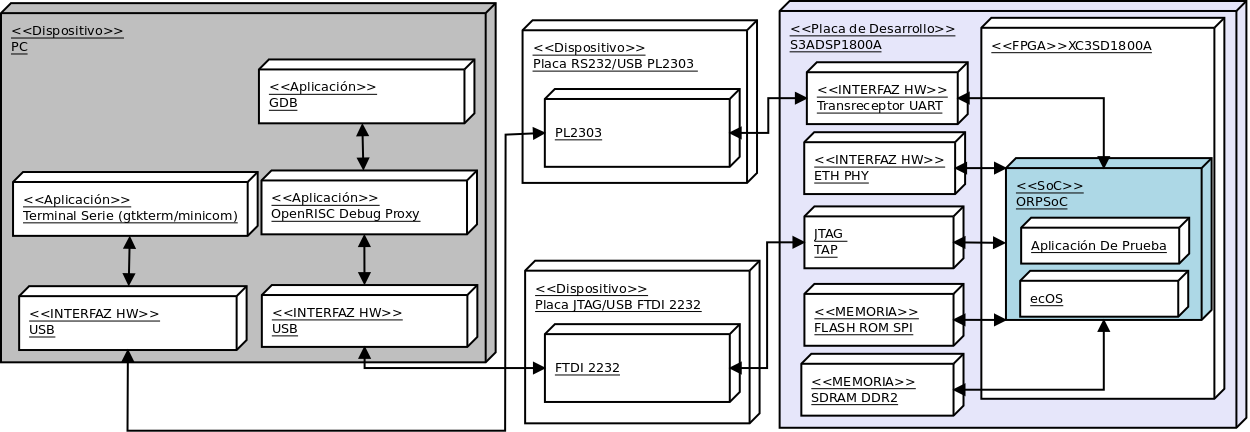
\includegraphics[width=1\textwidth,keepaspectratio=true]{./images/ecos}
  		\caption{Diagrama de Despliegue del Prototipo Tres}
  		\label{fig:ecos} 
 		\end{center}
		\end{figure}
	
		\section{Implementación}	
		
		La implementación de sistema operativo de tiempo real ecOS ser realiza en una serie de etapas detalladas a continuación. 
		\begin {itemize}
		\item Descarga del código fuente del proyecto
		\item Descarga de la aplicación de configuración de ecOS
		\item Instalación de dependencias de compilación
		\item Compilación de la herramienta de configuración
		\item Configuración del sistema
		\item Contrucción del sistema 
		\item Compilación de programas de prueba
		\item Ejecución de aplicaciones bajo ecOS
 		\end {itemize}
 
		Consulte la Guía de ecOS en el Anexo ~\ref{app:apendice4} para una comprensión más profunda de los pasos a seguir en la implementación sobre la
 		placa de desarrollo S3ADSP1800A.
		
\newpage
		%%%%%%%%%%%%%%%%%%%%%%%%%%%%TESTING TRES
		\section{Testing}

		\begin{table}[h!]
		\centering
		\begin{tabular}{ p{5cm} p{10cm}  }
		\hline 
		\rowcolor[gray]{0.8}  Caso de Prueba &  Interactuar correctamente con la interfaz UART\\
		\hline 
		Código de Requerimiento & RQX-PC 2\\ 
		\hline 
		Requerimiento & Se debe garantizar el correcto funcionamiento de todos los periféricos utilizando los driver y librerías provistas por el SO \\ 
		\hline 
		Código de Testing & T012\\ 
		\hline
		Propósito &  Comprobación del correcto funcionamiento del componente UART\\
		\hline
		Realizado Por & Gomez, Pablo \\
		\hline	
		Entorno de Ejecución & SO - ecOS\\
		\hline
		Precondiciones & \begin {itemize}
							\item Instanciación en la FPGA del SoC
							\item Ejecución de una terminal serie en la PC 
 							\item Comunicación establecida entre la placa de desarrollo y la PC
							\item Herramientas de compilación cruzada funcionando correctamente
							\item Sistema operativo correctamenta instalado
							\item Programas de prueba compilados correctamente
							\end {itemize} \\
		\hline
		Secuencia de Ejecución &  Ejecutación de la aplicación de prueba hello.elf\\
		\hline
		Postcondiciones &  El programa de prueba ejecutándose sobre el sistema operativo ecOS, lo que se manifiesta en la impresión de pantalla en la
		terminal serie de la PC\\
		\hline
 		\multicolumn{2}{>{\columncolor[gray]{.8}}c}{Resultados}\\
		\hline
		Resultados Esperados & Poder observar por la terminal serial una cadena de string \\
		\hline	
		Resultados Obtenidos & Al ejecutarse el programa de prueba pudo observarse la cadena string esperada "Hello, ecOS World"\\
		\hline
		\end{tabular}
		\end{table}

\newpage			


		\begin{table}[h!]
		\centering
		\begin{tabular}{ p{5cm} p{10cm}  }
		\hline 
		\rowcolor[gray]{0.8}  Caso de Prueba& Ejecución de hilos\\
		\hline 
		Código de Requerimiento & RQX-PC 3 , RQX-PC 4\\ 
		\hline 
		Requerimiento  	&  Se debe poder ejecutar programas que requiere la ejecución de múltiples hilos\\
		\hline 
						&  Problemas con el compilador para la generación del binario del programa de prueba\\
		\hline 
		Código de Testing & T014\\ 
		\hline
		Propósito &  Compilación y ejecución de un programa de prueba que ejecute hilos\\
		\hline
		Realizado Por & Lovaisa, Valeria \\
		\hline	
		Entorno de Ejecución & SO - ecOS \\
		\hline
		Precondiciones &    \begin {itemize}
							\item Instanciación en la FPGA del SoC.
							\item Ejecución de una terminal serie en la PC
							\item Comunicación establecida entre la placa de desarrollo y la PC
							\item Herramientas de compilación cruzada funcionando correctamente
							\item Sistema operativo correctamenta instalado
							\item Programas de prueba compilados correctamente
							\end {itemize}
		\\
		\hline
		Secuencia de Ejecución & Ejecución de la aplicación de prueba twothreads.elf \\
		\hline
		Postcondiciones & Aplicación ejecutándose sobre el sistema operativo \\
		\hline
 		\multicolumn{2}{>{\columncolor[gray]{.8}}c}{Resultados}\\
		\hline
		Resultados Esperados & Poder observar por la terminal serie el resultado de la ejecución de la aplicación\\
		\hline	
		Resultados Obtenidos & Al ejecutarse el programa de prueba de hilos pudo observarse la salida mostrada en la Referencia ~\ref{lst:salhilos} \\
		\hline
		\end{tabular}
		\end{table}

\newpage

\begin{lstlisting}[frame=single,caption={Salida de la ejecución del programa de prueba twothreads},label={lst:salhilos}]
PASS:<Thread 0 OK>
EXIT:<done>
\end{lstlisting}



\begin{lstlisting}[frame=single,caption={Salida de la ejecución del programa de prueba threads0},label={lst:salhilos}]
PASS:<Thread 0 OK>
EXIT:<done>
\end{lstlisting}



		\section{Conclusión}


\newpage
\chapter{Prototipo Cuatro : Implementación del SoC ORPSoC en FPGA con Sistema Operativos Linux}
		\section{Introducción}
		El núcleo Linux, combinado con un conjunto utilidades de software libre, puede ajustarse al espacio limitado de hardware 
	    de los sistemas embedidos. Una instalación típica de un Linux embebido ocupa en promedio 2 MB. En el prototipo cuatro se utilizó una versión
	    reducida del núcleo de Linux y herramientas provistas por el paquete BusyBox. 
		
		\section{Requerimientos del prototipo}
		
		\begin{table}[h!]
		\centering	
		\begin{tabular}{ p{2.5cm} p{8cm} p{3cm} }
		\hline 
		\rowcolor[gray]{0.8} N\textordmasculine Req  & Descripción\\
		\hline                             	RQX-PD 1 & El prototipo debe implementar el sistema operativos Linux\\ 
		\hline  						RQX-PD 2 & Se requiere la instalación de un gestor de arraque que posibilite el inicio del sistema operativo\\ 
		\hline 						RQX-PD 3 & Se debe poder grabar como aplicación firmware el gestor de arranque en la memoria flash SPI de la placa de desarrollo\\
		\hline 						RQX-PD 4 & El prototipo debe tener capacidad de ejecución de aplicaciones sobre el sistema operativo Linux\\
		\hline 
		\end{tabular}
		\end{table}
		
		
		\section{Matriz de Riesgo para el Prototipo Cuatro} 

		\begin{table}[h!]
		\centering
		\begin{tabular}{ p{2.5cm} p{9cm} p{2cm} p{2cm} }
		\hline 
		\rowcolor[gray]{0.8} N\textordmasculine Req Asociados  & Riegos Asociados & Severidad  & Ocurrencia \\
		\hline RQX-PC 1 & Fallas en la generación de la imagen del SO para ser montada en el SoC & Crítica       & Probable \\
		\hline			& Falta de documentación de apoyo para la implentación del SO bajo licencias de Software Libre & Crítico & Ocasional\\	
		\hline			& Limitaciones para la ejecución de SO de tiempo real & Crítico & Ocasional\\	
 		\hline RQX-PC 2 & Librerías necesarias inexistentes o con fallos& Crítico & Ocasional\\	
		\hline			& Drivers necesarios inexistentes o con fallos  & Severo  &  Ocasional\\ 
		\hline RQX-PC 3	& Problemas en la compilación e instalación de las herramientas de desarrollo de software& Severo  &  Ocasional\\ 
		\hline RQX-PB 4 & Problemas con el compilador para la generación del binario del programa de prueba  & Crítico&  Ocasional\\
		\hline
		\end{tabular}
		\caption{Tabla de Riegos vs. Requerimientos}
		%\label{tab:riegos}
		\end{table}

		\newpage

 		\begin{table}[h!]
		\centering
		\begin{tabular}{ p{4cm} p{4cm} p{4cm} p{3cm} }
		\hline 
		\rowcolor[gray]{0.8} Riesgo & Consecuencia & Estrategia preventiva & Estrategia de contingencia\\
		\hline Errores en la configuración de compilación del kernel para el SoC utilizado & 
		       Retraso en los tiempos de implementación & 
		       Análisis previo de archivos de configuración del SoC seleccionado o similares & 
		       Revisión y correción de archivos de configuración\\
		\hline Fallas en la generación de la imagen del SO y/o el gestor arranque para ser montada en el SoC & 
		       Retraso en los tiempos de implementación & 
		       Análisis previo de guías de resolución de problemas y preguntas frecuentes & 
		       Revisión de código y consulta a los desarrolladores\\
		\hline Falta de documentación de apoyo para la implentación del SO y/o gestor de arranque para la arquitectura OpenRISC & 
		       Demoras en la implementación del SO & 
		       Revisión previa de la documentación existente y guías de resolución de problemas & 
		       Mayor inversión de tiempo para la implementación\\
		\hline Falta de soporte del SO Linux y/o el gestor de arranque para su implementación en el hardware disponible & 
			   Fallos en la ejecución del sistema operativo & 
		       Análisis previo de limitaciones en la documentación de los desarrolladores y guías de resolución de problemas & 
		       Revisión y desarrollo de código del SO necesario para proveer soporte al hardware\\
		\hline Librerías necesarias inexistentes o con fallos & 
			   Imposibilidad de desarrollo de aplicaciones para ejecutar sobre el SO &
			   Análisis previo de las librerías disponibles y revisión de posibles bugs informados SO & 
			   Desarrollo de las librerías necesarias o corrección de errores\\
		\hline Drivers necesarios inexistentes o con fallos & 
			   Imposibilidad de utilización de los dispositivos necesarios & 
			   Análisis previo de los driver de los dispositivos a utilizar & 
			   Desarrollo de los drivers necesarios\\		
		\hline Problemas en la compilación e instalación de las herramientas de desarrollo de software & 
			   Imposibilidad de desarrollo de aplicaciones que se ejecuten sobre Linux Embebido & 
			   Verificación previa de la documentación de los desarrolladores y guías de resolución de problemas & 
			   Revisión de codigo y corrección de errores\\
		\hline
		\end{tabular}
		\caption{Planificación de riesgos}
		%\label{tab:planificación}
		\end{table}

		\newpage
		
		\section{Descripción de la Estructura del Prototipo Cuatro}
		Se muestra a continuación (Figura ~\ref{fig:proto4}) el diagrama de despliegue del prototipo cuatro. Se utiliza como base nuevamente el prototipo
		dos con un sistema operativo linux ejecutándose en él.

		\begin{figure}[h!]
 		\begin{center}
  		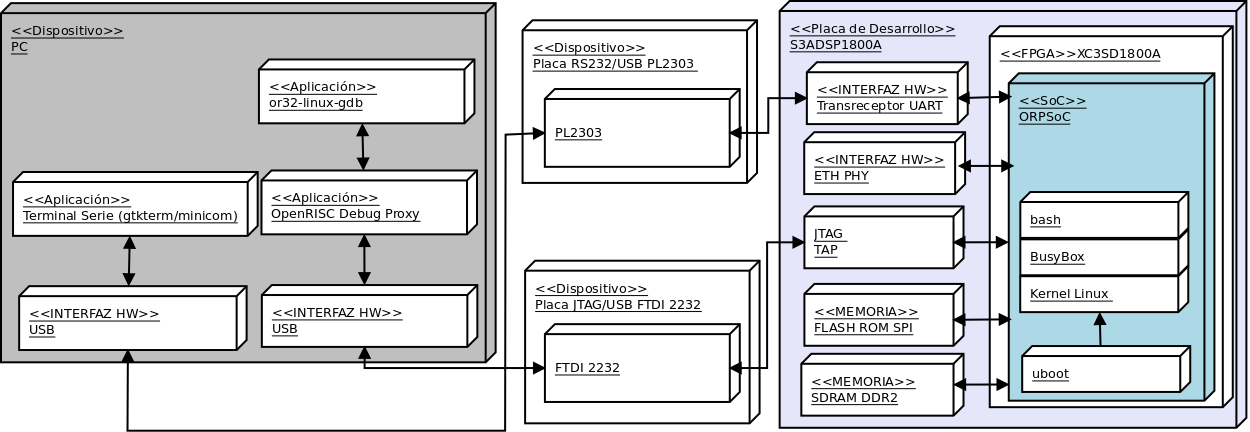
\includegraphics[width=1\textwidth,keepaspectratio=true]{./images/proto4}
  		\caption{Diagrama de Despliegue del Prototipo Cuatro}
  		\label{fig:proto4} 
 		\end{center}
		\end{figure}
	
		\newpage

		\section{Implementación}	
		
		\section{Testing}
		
		\begin{table}[h!]
		\centering
		\begin{tabular}{ p{5cm} p{10cm}  }
		\hline 
		\rowcolor[gray]{0.8} 	 Caso de Prueba & Carga de programa mediante el gestor de arranque UBoot\\
		\hline  		Código de Requerimiento 	& RQX-PD 2\\ 
		\hline  				  Requerimiento 	& Se requiere la instalación de un gestor de arraque que posibilite el inicio del sistema operativo\\
		\hline 				  Código de Testing & T015\\ 
		\hline 						  Propósito & Comprobación del correcto funcionamiento del gestor de arranque\\
		\hline					  Realizado Por & Lovaisa, Valeria \\
		\hline	 		   Entorno de Ejecución & Bare Metal\\
		\hline		   		   	 Precondiciones & \begin {itemize}
												  \item Instanciación en la FPGA del SoC ORPSoC
												  \item Ejecución de una terminal serie en la PC 
 												  \item Comunicación establecida entre la placa de desarrollo y la PC mediante Serial y eth
 												  \item Servidor TFTP funcionando correctamente sobre el SO host
												  \item Herramientas de compilación cruzada funcionando correctamente
												  \item Gestor de arranque y aplicación de prueba compilados correctamente
												  \item Imagen de arranque sin errores
												  \end {itemize} \\
		\hline			 Secuencia de Ejecución &  Ejecutación de la aplicación de prueba numprim.elf a través de Uboot\\
		\hline					Postcondiciones &  El gestor de arranque inicia correctamente el programa de prueba, lo que se manifiesta en la impresión de la salida
		del gestor de arranque y el programa prueba en la terminal serie de la PC\\
		\hline	\multicolumn{2}{>{\columncolor[gray]{.8}}c}{Resultados}\\
		\hline			   Resultados Esperados & Poder observar por la terminal serial las salida de los programas \\
		\hline	 		   Resultados Obtenidos & Al ejecutarse el programa de prueba pudo observarse la salida mostrada en la Referencia ~\ref{lst:salidauboot}\\
		\hline	
		\end{tabular}
		\end{table}

\newpage		
\begin{lstlisting}[frame=single,caption={Salida de la ejecución del programa de prueba cargado por uboot},label={lst:salidauboot}]
ACA va programa de prueba cargado por uboot

\end{lstlisting}
		
		\begin{table}[h!]
		\centering
		\begin{tabular}{ p{5cm} p{10cm}  }
		\hline 
		\rowcolor[gray]{0.8} 	 Caso de Prueba & Inicio del gestor de arranque desde la memoria Flash SPI\\
		\hline  		Código de Requerimiento & RQX-PD 3\\ 
		\hline  				  Requerimiento & Se debe poder grabar como aplicación firmware el gestor de arranque en la memoria flash SPI de la placa de desarrollo\\
		\hline 				  Código de Testing & T016\\ 
		\hline 						  Propósito & Verificación del inicio del gestor de arranque almacenado en la Flash SPI \\
		\hline					  Realizado Por & Lovaisa, Valeria \\
		\hline	 		   Entorno de Ejecución & Bare Metal\\
		\hline		   		   	 Precondiciones & \begin {itemize}
												  \item Instanciación en la FPGA del SoC ORPSoC
												  \item Ejecución de una terminal serie en la PC 
 												  \item Comunicación establecida entre la placa de desarrollo y la PC mediante Serial
 												  \item Herramientas de compilación cruzada funcionando correctamente
												  \item Gestor de arranque compilado correctamente
												  \item Imagen del gestor de arranque almacenada en la memoria Flash SPI de la placa de desarrollo
												  \end {itemize} \\
		\hline			 Secuencia de Ejecución &  Arranque inicial o reset del hardware\\
		\hline					Postcondiciones &  El gestor de arranque inicia correctamente , lo que se manifiesta en la impresión de la salida
		del gestor de arranque en la terminal serie de la PC\\
		\hline	\multicolumn{2}{>{\columncolor[gray]{.8}}c}{Resultados}\\
		\hline			   Resultados Esperados & Poder observar por la terminal serial las salida del Uboot \\
		\hline	 		   Resultados Obtenidos & Al ejecutarse el programa de prueba pudo observarse la salida mostrada en la Referencia ~\ref{lst:salidaspi}\\
		\hline	
		\end{tabular}
		\end{table}

\begin{lstlisting}[frame=single,caption={Salida de la ejecución del programa de prueba cargado por uboot},label={lst:salidauboot}]
aca va  
\end{lstlisting}		

		\begin{table}[h!]
		\centering
		\begin{tabular}{ p{5cm} p{10cm}  }
		\hline 
		\rowcolor[gray]{0.8} 	 Caso de Prueba & Implementación del SO Linux Embebido\\
		\hline  		Código de Requerimiento & RQX-PD 1\\ 
		\hline  				  Requerimiento & El prototipo debe implementar el sistema operativos Linux\\
		\hline 				  Código de Testing & T017\\ 
		\hline 						  Propósito & Implementar correctamente un Sistema Operativo Linux Embebido sobre un SoC ORPSoC\\
		\hline					  Realizado Por & Lovaisa, Valeria \\
		\hline	 		   Entorno de Ejecución & Bare Metal\\
		\hline		   		   	 Precondiciones & \begin {itemize}
												  \item Instanciación en la FPGA del SoC ORPSoC
												  \item Ejecución de una terminal serie en la PC 
 												  \item Comunicación establecida entre la placa de desarrollo y la PC
 												  \item Herramientas de compilación cruzada funcionando correctamente
 												  \item Configuración del kernel adaptada al SoC
												  \item Imágen del Sistema Operativo Linux compilada correctamente 
												  \end {itemize}\\
		\hline			 Secuencia de Ejecución & Inicio del Sistema Operativo \\
		\hline					Postcondiciones & Se inicia correctamente el Sistema Operativo, lo que se manifiesta en la impresión de la salida
		de la secuencia de arranque de linux en la terminal serie de la PC\\
		\hline	\multicolumn{2}{>{\columncolor[gray]{.8}}c}{Resultados}\\
		\hline			   Resultados Esperados & Lograr observar por la terminal serial la secuencia de arranque del Sistema Operativo\\
		\hline	 		   Resultados Obtenidos & Al ejecutarse el programa de prueba pudo observarse la salida mostrada en la Referencia ~\ref{lst:sallinux}\\
		\hline	
		\end{tabular}
		\end{table}
		
\begin{lstlisting}[frame=single,caption={Salida de la secuencia de incio de Linux Embebido},label={lst:sallinux}]
 ACA VA EL RESULTADO DE CORRER UBOOT DESDE LA SPI
\end{lstlisting}		
		
		\begin{table}[h!]
		\centering
		\begin{tabular}{ p{5cm} p{10cm}  }
		\hline 
		\rowcolor[gray]{0.8} 	 Caso de Prueba & Ejecución de aplicaciones de prueba sobre Linux\\
		\hline  		Código de Requerimiento & RQX-PD 4\\ 
		\hline  				  Requerimiento & El prototipo debe tener capacidad de ejecución y depuración de aplicaciones sobre el sistema operativo Linux\\
		\hline 				  Código de Testing & T018\\ 
		\hline 						  Propósito & Ejecución de aplicaciones de prueba sobre entorno Linux\\
		\hline					  Realizado Por & Lovaisa, Valeria \\
		\hline	 		   Entorno de Ejecución & Linux\\
		\hline		   		   	 Precondiciones & \begin {itemize}
												  \item Instanciación en la FPGA del SoC ORPSoC
												  \item Ejecución de una terminal serie en la PC 
 												  \item Comunicación establecida entre la placa de desarrollo y la PC
 												  \item Herramientas de compilación cruzada para su ejecución sobre Linux funcionando correctamente
												  \item SO Linux ejecutándose correctamente sobre el SoC ORPSoC 
												  \end {itemize} \\
		\hline			 Secuencia de Ejecución & \begin {itemize}
						 					 	  \item Inicio del gestor de arranque
												  \item Inicio del Sistema Operativo
												  \item Ejecución de la aplicación de prueba
						 						  \end {itemize} \\
		\hline					Postcondiciones &  Se ejecuta correctamente el programa de prueba, lo que se manifiesta en la impresión de la salida
		del bash de linux en la terminal serie de la PC\\
		\hline	\multicolumn{2}{>{\columncolor[gray]{.8}}c}{Resultados}\\
		\hline			   Resultados Esperados & Poder observar por la terminal serial las salida de ejecución del programa de prueba \\
		\hline	 		   Resultados Obtenidos & Al ejecutarse el programa de prueba pudo observarse la salida mostrada en la Referencia ~\ref{lst:salidalinux}\\
		\hline	
		\end{tabular}
		\end{table}

\begin{lstlisting}[frame=single,caption={Salida de la ejecución del programa de prueba ejecutado en Linux Embebido},label={lst:salidalinux}]
 ACA VA EL RESULTADO DE CORRER UBOOT DESDE LA SPI
\end{lstlisting}		
		
		\section{Conclusión}
 % Implementacion y Diseño
\newpage
\end{part}
\begin{part}{Presentación de Resultados y Conclusiones Finales}
\newpage
\chapter{Resultados} \label {chap:resultados}
	\section{Introducción} 
	
	Este capítulo presenta los resultados obtenidos durante la implementación de cada uno de los prototipos planteados en el Capítulo
	~\ref{chap:disenoeimpl} y durante la ejección de los casos de prueba correspondientes. 
\begin{itemize}
\item Se instanciaron los proyectos MinSoC y ORPSoC, ambos con núcleo OpenRISC. 
\item Se evaluó el funcionamiento del microprocesador OpenRISC con programa de prueba de multiplicación de matrices binarias cuadradas.
\item Se evaluaron las capacidades del compilador cruzado or32-elf-gcc en lo referido a su capacidad de optimización de código. 
\item Se ejecutaron los benchmarks de sistemas embebidos \verb|coremark| y \verb|dhrystone| para posicionar el microprocesador OpenRISC entre CPUs de similares
características.
\item Se realizó la implementación de dos sistemas operativos, uno de tiempo real (ecOS) y uno de mayores capacidades (Linux). 
\end{itemize}				
				
	Para la ejecución de todas las pruebas se utilizó la placa desarrollo S3ADSP1800A del fabricante Xilinx que cumple con los requerimientos detallados
	en la tabla~\ref{tab:requsr1} y se encontraba dentro de las alternativas disponibles al momento del desarrollo de este trabajo. Durante el desarrollo de las pruebas se pretendió establecer los límites de aplicación del proyecto
	que establezcan referencias sólidas para una futura elección del proyecto en aplicaciones reales.


	\newpage
	\section{Resultados de Utilización de FPGA en la Implementación del Proyecto MinSoC}

El proyecto MinSoC se encuentra enfocado a su utilización en sistemas embebidos de capacidades ajustadas sintetizables en una gran cantidad de FPGA de diversos desarrolladores. En la tabla ~\ref{tab:conbench} se presentan con éxito la implemantación del proyecto en uno de los kit de desarrollo soportado por el proyecto y disponible para su uso en el laboratorio CUDAR.

\begin{table}[h!]
		\begin{tabular}{ |p{6cm} |p{3cm} |p{3cm}| p{3cm}| }    
		\hline
		\multicolumn{4}{|>{\columncolor[gray]{.8}}c}{Resumen de utilización MinSoC}\\
		\hline
		\multicolumn{1}{|>{\columncolor[gray]{.8}}c}{Logica utilizada} & \multicolumn{1}{|>{\columncolor[gray]{.8}}c}{Usado} & \multicolumn{1}{|>{\columncolor[gray]{.8}}c}{Disponible} & \multicolumn{1}{|>{\columncolor[gray]{.8}}c}{Utilizado} \\
		\hline 
		Slice Flip Flop & 5040 & 33280 & 15\%  \\ 
		\hline 
		LUTs de 4 entradas & 13901 & 33280 & 41\%  \\ 
		\hline 
\multicolumn{1}{|>{\columncolor[gray]{.8}}c}{Logica de distribución} & \multicolumn{1}{|>{\columncolor[gray]{.8}}c}{Usado} & \multicolumn{1}{|>{\columncolor[gray]{.8}}c}{Disponible} & \multicolumn{1}{|>{\columncolor[gray]{.8}}c}{Utilizado} \\
		\hline 
		Slice & 8475 & 16640 & 50\%  \\ 
		\hline 
		Luts de 4 entradas para lógica combinacional& 13866 & 33280 & 40\%  \\ 
		\hline 
		Luts de 4 entradas route-thru & 330 & 33280 & 1\%  \\ 		
		\hline 
		Luts de 4 entradas para puertos Dual RAM & 32 & 33280 & 0,9\%  \\ 		
		\hline 
		Luts de 4 entradas para shift registers & 3 & 33280 & 0,1\%  \\ 
		\hline
		IOBs& 29 & 519 & 5\%  \\ 
		\hline 
		BUFGMUXs & 5 & 24 & 20\%  \\ 
		\hline 
		DCMs & 1 & 8 & 12\%  \\ 
		\hline
		DSP48As & 4 & 84 & 4\%  \\ 
		\hline 
		RAMB16BWERs & 70 & 84 & 83\%  \\ 
		\hline 
		BSCAN\_SPARTAN3As& 1 & 1 & 100\%  \\ 
		\hline 
\end{tabular}
%\end{center}
\caption{Resultados de la implementación del proyecto MinSoC}
\label{tab:conbench}
\end{table}

Como se puede observar los resultados obtenidos luego del proceso completo de implementación del proyecto MinSoC, desde el punto de vista de utilización lógica se utilizó el 15\% de Slice Flip Flops y el 41\% de LUTs disponibles en la FPGA.  Respecto de la distribución lógica se tiene un 50\% de ocupación de Slices y un 42\% de LUTs de 4 entradas de las cuales el 1\% se utiliza
	como LUTs de paso o en inglés route-thru. El 41\% restante están utilizadas como lógica combinacional , puertos Dual RAM y registros de
	desplazamiento. Se utilizó el 5\% de los bloques de entrada/salida, el 20\% de los BUFGMUXs ó buffers de clock global, el 12\% de los DCMs, el 4\% de
	los bloques DSP y el 83\% de los bloques de RAM. El proceso Technology Mapping utilizó un pico 415 MB de memoria.

Teniendo en cuenta los datos obtenidos y la facilidad de adaptación del proyecto para portarse a otras arquitecturas reconfigurables, se pueden aproximar los límites de la aplicación del proyecto para el uso mas eficiente de los recursos provistos de una futura elección en placas de desarrollo, derivando esto, por ejemplo en reducción de costos.


\newpage
	\section{Resultados de Utilización de FPGA en la Implementación del Proyecto ORPSoC}

El proyecto ORPSoC también se encuentra enfocado a su utilización en sistemas embebidos de capacidades ajustadas sintetizables en una gran cantidad de FPGA de diversos desarrolladores. A continuación en la tabla~\ref{tab:conbench1} se presentan con éxito la  implementación del proyecto sobre el kit de desarrollo de Xilinx.
		
\begin{table}[h!]
		\begin{tabular}{ |p{6cm} |p{3cm} |p{3cm}| p{3cm}| }    
		\hline
		\multicolumn{4}{|>{\columncolor[gray]{.8}}c}{Resumen de utilización ORPSoC}\\
		\hline
		\multicolumn{1}{|>{\columncolor[gray]{.8}}c}{Logica utilizada} & \multicolumn{1}{|>{\columncolor[gray]{.8}}c}{Usado} & \multicolumn{1}{|>{\columncolor[gray]{.8}}c}{Disponible} & \multicolumn{1}{|>{\columncolor[gray]{.8}}c}{Utilizado} \\
		\hline 
		Slice Flip Flop & 4872 & 33280 & 14\%  \\ 
		\hline 
		LUTs de 4 entradas & 12093 & 33280 & 36\%  \\ 
		\hline 
\multicolumn{1}{|>{\columncolor[gray]{.8}}c}{Logica de distribución} & \multicolumn{1}{|>{\columncolor[gray]{.8}}c}{Usado} & \multicolumn{1}{|>{\columncolor[gray]{.8}}c}{Disponible} & \multicolumn{1}{|>{\columncolor[gray]{.8}}c}{Utilizado} \\
		\hline 
		Slice &7772 & 16640 & 46\%  \\ 
		\hline 
		Luts de 4 entradas para lógica combinacional& 11009 & 33280 & 33\%  \\ 
		\hline 
		Luts de 4 entradas route-thru & 250 & 33280 & 0,7\%  \\ 		
		\hline 
		Luts de 4 entradas para puertos Dual RAM & 960 & 33280 & 3\%  \\ 		
		\hline 
		Luts de 4 entradas para Shift registers & 124 & 33280 & 0,3\%  \\ 
		\hline 		
		IOBs& 128 & 519 & 24\%  \\ 
		\hline  
		BUFGMUXs & 7 & 24 & 29\%  \\ 
		\hline 
		DCMs & 2 & 8 & 25\%  \\ 
		\hline
		DSP48As & 4 & 84 & 4\%  \\ 
		\hline 
		RAMB16BWERs & 16 & 84 & 19\%  \\ 
		\hline 
		BSCAN\_SPARTAN3As& 1 & 1 & 100\%  \\ 
		\hline 
\end{tabular}
%\end{center}
\caption{Resultados de la implementación del proyecto ORPSoC}
\label{tab:conbench1}
\end{table}	
		
	Como se puede observar que desde el punto de vista de utilización lógica se utilizó el 14\% de Slice Flip Flops y el 36\% de LUTs disponibles en
	la FPGA. Respecto de la distribución lógica se tiene un 46\% de ocupación de Slices y un 37\% de LUTs de 4 entradas de las cuales el 0,7\% se utiliza
	como LUTs de paso o en inglés route-thru. El 36\% restante están utilizadas como lógica combinacional , puertos Dual RAM y registros de
	desplazamiento. Se utilizó el 24\% de los bloques de entrada/salida, el 29\% de los BUFGMUXs ó buffers de clock global, el 25\% de los DCMs, el 4\%
	de los bloques DSP y el 19\% de los bloques de RAM. El proceso Technology Mapping utilizó un pico 410 MB de memoria.  
 
Al igual que en la implemetación del proyecto anterior en la placa de desarrollo de Xilinx,  teniendo en cuenta la capacidad de adaptación a otras arquitecturas reconfigurable que tiene el proyecto ORPSoC, con los datos obtenidos se llego a la conclusión de que seria viable implemtarlo en placas mas pequeñas y de menor costo.

%		\subsection{Reporte de timing}	
%
%El reporte de timing presenta los resultados del análisis de distribución de los clocks del proyecto. Entre los resultados se obtiene el mínimo
%periodo (Máx Frecuencia) necesarios para el correcto funcionamiento del sistema. Es importante destacar que los tiempos expuestos en el reporte son
%teóricos y se presentan cambios importante durante las pruebas sobre el hardware. 
%
%\begin{lstlisting}[frame=single,caption={Reporte timing - ORPSoC},label={lst:salidas},breaklines]
%Timing summary:
%
%Timing errors: 498  Score: 729028  (Setup/Max: 311057, Hold: 417971)
%Constraints cover 395663179 paths, 94 nets, and 53193 connections
%
%Design statistics:
%  Minimum period:  45.166ns   (Maximum frequency:  22.141MHz)
%  Maximum path delay from/to any node:  11.696ns
%  Maximum net delay:   2.594ns
%  Minimum input required time before clock:  26.237ns
%  Maximum output delay after clock:  13.126ns
%\end{lstlisting}



\newpage
\section {Estudio de Capacidades del Proyecto MinSoC}
		
		\subsection{Estudio de la complejidad del algoritmo de prueba}
		
		El tiempo de ejecución de un algoritmo va a depender de diversos factores como son: los datos de entrada que le suministremos, la calidad del
		código generado por el compilador para crear el programa objeto, la naturaleza y rapidez  de las instrucciones máquina del procesador concreto que
		ejecute el programa y la complejidad intrínseca del algoritmo. Hay dos estudios posibles sobre el tiempo: 
 
		\begin{itemize}
		  \item Uno que proporciona una medida teórica (a priori), que consiste en obtener una  función que acote (por arriba o por abajo) el tiempo de
		  ejecución del algoritmo para unos valores de entrada dados.
		\item Y otro que ofrece una medida real (a posteriori), consistente en medir el tiempo  de ejecución del algoritmo para unos valores de entrada
		dados y en un ordenador concreto. 
		\end{itemize} 
		
		Entendemos por tamaño de la entrada el número de componentes sobre los que  se va a ejecutar el algoritmo. Por ejemplo, la dimensión del vector a
		ordenar o el tamaño de las matrices a multiplicar. La unidad de tiempo a la que debe hacer referencia estas medidas de eficiencia  no puede 
		expresarse en segundos o en otra unidad de tiempo concreta, pues no existe un ordenador estándar al que puedan hacer referencia todas las medidas. 
        Denotaremos por T(n) el tiempo de ejecución de un algoritmo para una entrada de tamaño n. 
        
        También es importante hacer notar que el comportamiento de un algoritmo puede cambiar notablemente para diferentes entradas (por ejemplo, los
        ordenados que se encuentren ya los datos a ordenar). De hecho, para muchos programas el tiempo de ejecución es en realidad una función de la
        entrada específica, y no sólo del tamaño de ésta. Así suelen estudiarse tres casos para un mismo algoritmo: caso peor, caso mejor y caso
        medio. El caso mejor corresponde a la traza (secuencia de sentencias) del algoritmo que realiza menos instrucciones. Análogamente, el caso
        peor corresponde a la traza del algoritmo que realiza más instrucciones.
 		
 		A la hora de medir el tiempo, siempre lo haremos en función del número de operaciones elementales que realiza dicho algoritmo, entendiendo por
 		operaciones elementales (en adelante OE) aquellas que el ordenador realiza en tiempo acotado por una constante. Así, consideraremos OE las
 		operaciones aritméticas básicas,  asignaciones a variables de tipo predefinido por el compilador, los saltos (llamadas a funciones y
 		procedimientos, retorno desde ellos, etc.), las comparaciones lógicas y el acceso a estructuras indexadas básicas, como son los vectores y
 		matrices. Cada una de ellas contabilizará como 1 OE. Resumiendo, el tiempo de ejecución de un algoritmo va a ser una función que mide el número de
 		operaciones elementales que realiza el algoritmo para un tamaño de entrada dado.
		
		Se define a continuación la complejidad de cálculo para el multiplicador de matrices binarias implementado en la sección ~\ref {testing:proto1} que
		cuenta con tres bucles anidados y operaciones de multiplicación y acumulación.
	
\newpage			
	\begin{lstlisting}[language=C,frame=single , caption={Código del programa de prueba multiplicador de matrices binarias}]
for (i=0;i<indice;i++){						(*1*)
  for (j=0;j<indice;j++){					(*2*)
    for (k=0;k<indice;k++){					(*3*)
	  producto = matrizA[i*con+k] * matrizB[k*con+j];	(*4*)
	  acumulador = acumulador + producto;			(*5*) 
    }								(*6*)
  matriz [i*con+j] = acumulador;				(*7*)
  acumulador = 0;						(*8*)
  }								(*9*)
}								(*10*)
	\end{lstlisting}
		
	    Para determinar el tiempo de ejecución, calcularemos primero el número de operaciones elementales (OE) que se realizan: 
 		\begin{itemize}
 		  \item Línea (1) En la primera iteración del bucle si tiene una asignación. Luego se efectúa la condición del bucle que depende de ``i'' con
 		  una comparación y un post incremento de i. (2 OE)
 		  \item Línea (2) En la primera iteración del bucle si tiene una asignación. Se efectúa la condición del bucle que depende de ``j'' con una
 		  comparación y un post incremento de j. (2 OE)
 		  \item Línea (3) En la primera iteración del bucle si tiene una asignación. Se efectúa la condición del bucle que depende de ``k'' con una
 		  comparación y un post incremento de k. (2 OE)
 		  \item Línea (4) está compuesta por una asignación, dos accesos a vectores, dos incrementos y tres productos. (8 OE) 
 		  \item Línea (5) está compuesta por una asignación y una suma (2 OE)
 		  \item Línea (6) se tiene fin del bucle que depende de ``k'' (1 OE)
 		  \item Línea (7) se tiene una asignación , un incremento, un producto y un acceso a vector (4 OE)
 		  \item Línea (8) se tiene una asignación (1 OE)
 		  \item Línea (9) se tiene fin del bucle que depende de ``j'' (1 OE)
 		  \item Línea (10) se tiene fin del bucle que depende de ``i'' (1 OE)
 		\end{itemize}
		
		Se establece que indice = n (todas matrices cuadradas nxn). Se tiene entonces: 
		
		\begin{equation*}
		T(n) = 1 + \sum_{i=0}^{n-1} \left (2 + \sum_{j=0}^{n-1} \left (2 + \sum_{k=0}^{n-1} 1 + (8+2)\right ) + (4 + 1) \right )      
		\end{equation*}
		
		Obteniendo de esta manera:
		
		\begin{equation*}
		T(n) = 11 n^3 + 9 n^2 + 1       
		\end{equation*}
		 
		
		\subsection{Resultados de la ejecución del multiplicador de matrices binarias}
			
		Se presentan a continuación los resultados de ejecución del programa multiplicador de matrices binarias. Se utilizó un gráfico que muestra el orden
		de las matrices multiplicadas vs. la cantidad de ticks de ejecución. El figura~\ref{fig:mulmat} muestra con claridad que el tiempo de ejecución
		aumenta exponencialmente a medida que aumenta el orden de las matrices multiplicadas.
		
\begin{figure}[h!]
 	\begin{center}
  	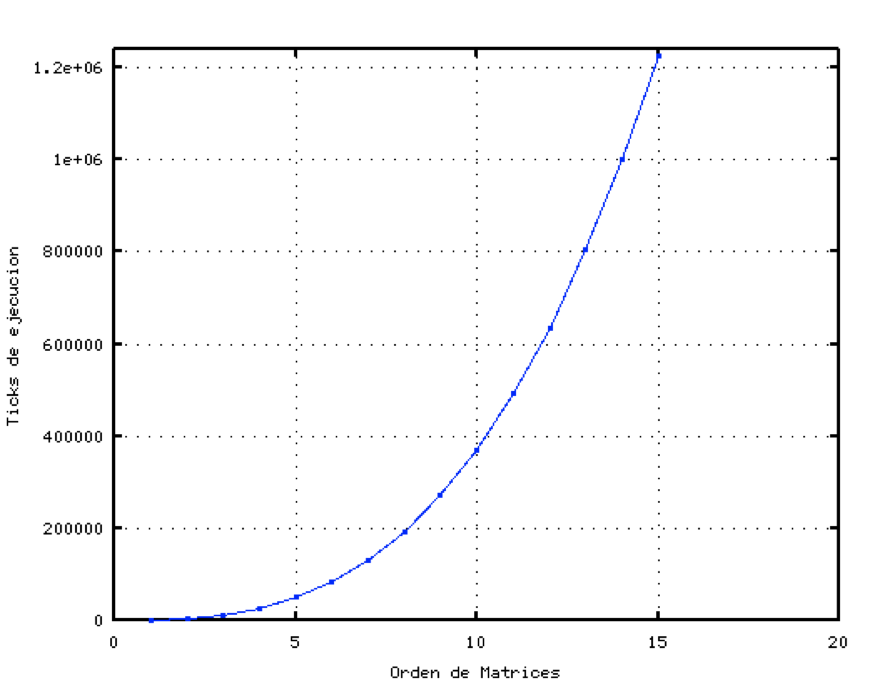
\includegraphics[width=0.9\textwidth,keepaspectratio=true]{./images/calculomatriz}
  	\caption{Multiplicación de matrices binarias}
  	\label{fig:mulmat}
 	\end{center}
	\end{figure}

		Teniendo en cuenta que la aplicación ejecutó en una versión sintentizada básica del proyecto minSoC, este no posee unidades de multiplicación
		por hardware que efectuen cálculos con mayor eficiencia, reduciendo el tiempo de ejecución. Pueden considerarse también, las optimizaciones del
		compilador, pero este aspecto fue analizado en el Prototipo Tres con mayor detalle. 	

        \subsection{Estudio de los niveles y banderas de optimización del compilador cruzado}
		\subsubsection{Optimización de código}
		
El objetivo de la optimización de código por parte del compilador es obtener código que se ejecuta más eficientemente según los criterios:
\begin{itemize}
  \item Tiempo de ejecución (optimización temporal)
  \item Espacio de memoria utilizado (optimización espacial) 
\end{itemize}
 
El funcionamiento básico de este mecanismo consiste en que el compilador revisa el código generado a varios niveles de abstracción y realiza las
optimizaciones aplicables al nivel de abstracción.
\begin{itemize}
  	\item Árbol sintáctico abstracto: optimizar subexpresiones redundantes, reducción de frecuencia, etc.
	\item Tuplas o cuadruplas: optimizar el uso de los registros o de las variables temporales.
	\item Ensamblador/Código máquina: convertir saltos a saltos cortos, reordenar instrucciones
\end{itemize}

Se define un bloque básico como un fragmento de código que tiene una única entrada y salida, y cuyas instrucciones se ejecutan secuencialmente. Si se
ejecuta una instrucción del bloque se ejecutan todas en un orden conocido en tiempo de compilación. La idea del bloque básico es encontrar partes del programa
cuyo análisis necesario para la optimización sea lo más simple posible.

Una técnica bien conocida para la optimización de bucles es la llamada desenrrolado de bucles (Loop Unrolling). La expansión de bucles solo se puede
aplicar a los bucles cuyo número de iteraciones se conoce en tiempo de compilación. La expansión de un bucle puede ser muy costosa en espacio. Hay
que poner un criterio heurístico para decidir si se aplica la expansión. Se puede aplicar una expansión parcial en la que sigue existiendo el bucle,
pero cada iteración del nuevo bucle corresponde a varias iteraciones del bucle original. En un bucle expandido se ha de sustituir el índice del bucle 
por el valor constante correspondiente.

El compilador cruzado utilizado en este trabajo or32-elf-gcc Versión 4.5.1 permite realizar optimizaciones de código mediante una serie de flags que
identifican cada uno de los mecanismos de optimización que el compilador implementa. Los flags fueron utilizados durante la ejecución de pruebas en
este trabajo son:

\begin{itemize}
  	\item -O2 : Este nivel de optimización activa una serie de flags que pueden consultarse en \cite{etiqueta_OptGcc}, una características de este nivel es que baja las restricciones en las operaciones con punto flotante.
	\item -O3 : Este nivel de procura una mayor optimización de código y activa una serie de flags conjunto con los del nivel -O2 que pueden consultarse
	en \cite{etiqueta_OptGcc}
	\item -funroll-loops : Desenrrolla los bucles cuyo número de iteraciones puede ser determinado en tiempo de compilación. 
	\item -funroll-all-loops : Desentrolla todos los bucles aún cuando el número de iteraciones no pueda determinarse en tiempo de compilación. 
	\item -fgcse-sm : Cuando este flag se encuentra activado, el compilador procura mover fuera de los bucles las operaciones store.
\end{itemize}

		\subsubsection{Resultados de la compilación de un bucle simple}

A modo de prueba se planteó un programa que incluye un arreglo de elementos enteros y dos bucles ``for'' , uno para la inicialización del arreglo y
otro para su actualización.

	\begin{lstlisting}[language=C,frame=single , caption={Código del programa de prueba de opciones de optimización del compilador (bucle simple) }]
#define ITERACIONES 1000
#define CTE 3

int x [ITERACIONES];
int i ;

void set (){
	for (i=0;i<ITERACIONES;i++)
		x[i] = 4;
}

void calc () {
	for (i=0;i<ITERACIONES;i++)
		x[i] = x[i] + CTE;
}

void main () {
	set ();
	calc ();
}
	\end{lstlisting}
		
En una primera instancia se realizó el desensamblado del binario generado para las funciones set (inicialización) y calc (actualización) con un
numero de 1000 iteraciones y para cada uno de los flags de optimización. Los códigos generados pueden observarse en detalle en el apéndice~\ref{chap:CodPrueba}. 
\newpage		
A continuación se presenta en la tabla~\ref{tab:conbench2} el resume de los resultados obtenidos para 1000 iteraciones y diversos flags de optimización:

\begin{table}[!h]
		\centering
		\begin{tabular}{ | p{4cm} | p{5cm} | p{2.5cm} | p{2cm} | }
		\hline 
		\rowcolor[gray]{0.8} Función & Flags & Cantidad de Instrucciones  & Registros Utilizados \\    
		\hline 
		set (inicialización) 	& -O2 						& 19 &  4 \\ 
		\hline 
							 	& -O2 -funroll-loops 		& 25 &  7 \\ 
		\hline 
							 	& -O2 -funroll-all-loops 	& 25 &  7 \\ 
		\hline 
							 	& -O3 						& 19 &  4 \\ 
		\hline 
							 	& -O3 -funroll-loops 		& 25 &  7 \\ 
		\hline 
							 	& -O3 -funroll-all-loops 	& 25 &  7 \\ 
		\hline 
		calc (actualización) 	& -O2						& 19 &  4 \\ 
		\hline 
							 	& -O2 -funroll-loops 		& 47 &  20 \\ 
		\hline 
							 	& -O2 -funroll-all-loops 	& 47 &  20 \\ 		
		\hline					 	
							 	& -O3 						& 19 &  4 \\ 
		\hline 
							 	& -O3 -funroll-loops 		& 47 &  20 \\ 
		\hline 
							 	& -O3 -funroll-all-loops 	& 47 &  20 \\ 		
		\hline 
		\end{tabular}
\caption{Resultados de la compilación del programa de prueba con diversos flags de optimización}
\label{tab:conbench2}
\end{table}	

%\newpage		

\section {Estudio de Capacidades del Proyecto ORPSoC}	
		\subsection{Condiciones de entorno de ejecución para benchmark}
		
		En la siguente tabla~\ref{tab:conbench} se muestran las condiciones del entorno de prueba durante los benchmarks.  

		\begin{table}[h!]
		\begin{tabular}{ |p{5cm} |p{10cm}| }    
		\hline
		\multicolumn{2}{|>{\columncolor[gray]{.8}}c}{Condiciónes de entorno de prueba|}\\
		\hline
		Placa de desarrollo & S3ADSP1800A  \\
		\hline 
		FPGA & Xilinx Spartan-3 XC3SD1800A \\ 
		\hline 
		Reloj del procesador & 25 MHz\\ 
		\hline
		Caché de instrucciones  & 8 KB \\ 
		\hline
		Caché de datos	  & 8 KB\\ 
		\hline	
		MMU & Sí \\	
		\hline
		Multiplicador hardware & Sí \\		
		\hline	
		División hardware & Sí \\		
		\hline	
		Punto Flotante & Precisión simple \\		
		\hline
\end{tabular}
%\end{center}
\caption{Condiciones del entorno de prueba}
\label{tab:conbench}
\end{table}


		\subsection{Resultados de la ejecución del benchmark CoreMark}
		

Inicialmente el benchmark CoreMark arroja como resultado un valor de 0,49/MHz, sin ningún tipo de optimización. Luego se presentan en la tabla~\ref{tab:conbench2} los resultados obtenidos durante la ejecución del benchmark CoreMark compilado con los optimizadores de nivel 2 (-O2) y nivel 3 (-O3) del compilador cruzado. 

%	\subsection {Presentación de los resultados de optimización} 
% 41.288895(iteracions/segundos)/25MHz =1.65coremark/Mhz

\begin{table}[!h]
\begin{center}
\begin{tabular}{ |l |c |c |c |c|}
\hline
\rowcolor[gray]{0.8} Opciones del compilador&-O2& Optimización &-O3& Optimización \\
\hline
Sin extras 					& 1.41 	& 			& 1.45 &  \\
\hline
-mhard-div -mhard-mu 		& 1.41	& 0\%		& 1.45 & 0\% \\
\hline
-funroll-loops			 	& 1.53	& 8\%		& 1.50 & 4\%\\
\hline
-fgcse-sm					& 1.42	& 0,7\%		& 1.46 & 0,6\%\\
\hline
-msoft-float 				& 1.41	& 0\%		& 1.45 & 0\%\\
\hline
-funroll-all-loops	 		& 1.55	& 10\%		& 1.52 & 5\%\\
\hline
Todos	 					& 1.55	& 10\%		& 1.52 & 5\%\\
\hline
\end{tabular}
\end{center}
\caption{Compilación con distintos niveles y flags de optimización}
\label{tab:conbench2}
\end{table}

Se puede observar que se mejoró el valor del CoreMark para un nivel de optimizacion -O2 en un 65\% y para un nivel de optimización -O3 en un 66\% con respecto al valor sin ningún tipo de optimización. Esta diferencia de mas del 65\% para un nivel de optimizador -02 era esperada, teniendo en cuenta que CoreMarks tiene operaciones con punto flotante, por lo tanto vale la pena realizar la optimización. Luego agregando flags en cada nivel de compilación se pudo obtener para un nivel de optimización -O2 una mejora del 10\% y para un nivel de optimización -O3 una mejora del 5\%  con respecto el valor obtenido sin ningún flag habilitado en cada nivel de optimización. 


%  A continuación se muestran en el bloque ~\ref{lst:salidasO2} algunas de las salidas que resultan de ejecutar el CoreMark compilado con el nivel de optimización -O2, -O3 y diferentes flags de optimización se observaron los resultados mostrados en el bloque ~\ref{lst:salidasO2}
% 
% \begin{lstlisting}[frame=single,caption={Optimización nivel -O2 - Flags activos : -FUNROLL-LOOPS },label={lst:salidasO2},breaklines]
% 2K validation run parameters for coremark.
% CoreMark Size    : 666
% Total ticks      : 1527
% Total time (secs): 15.270000
% Iterations/Sec   : 39.292731
% Iterations       : 600
% Compiler version : GCC4.5.1-or32-1.0rc4
% Compiler flags   : -O2  -mboard=s3adsp1800a -FUNROLL-LOOPS -DVALIDATION_RUN=1  
% \end{lstlisting}
% 
% \begin{lstlisting}[frame=single,caption={Optimización nivel -O2 - Flags activos : -MSOFT-FLOAT},label={lst:salidas},breaklines]
% 2K validation run parameters for coremark.
% CoreMark Size    : 666
% Total ticks      : 1528
% Total time (secs): 15.280000
% Iterations/Sec   : 39.267016
% Iterations       : 600
% Compiler version : GCC4.5.1-or32-1.0rc4
% Compiler flags   : -O2  -mboard=s3adsp1800a -MSOFT-FLOAT -DVALIDATION_RUN=1  
% \end{lstlisting}
% 
% \begin{lstlisting}[frame=single,caption={Optimización nivel -O2 - Flags activos : -FUNROLL-ALL-LOOPS},label={lst:salidas},breaklines]
% 2K validation run parameters for coremark.
% CoreMark Size    : 666
% Total ticks      : 1528
% Total time (secs): 15.280000
% Iterations/Sec   : 39.267016
% Iterations       : 600
% Compiler version : GCC4.5.1-or32-1.0rc4
% Compiler flags   : -O2  -mboard=s3adsp1800a -FUNROLL-ALL-LOOPS -DVALIDATION_RUN=1  
% \end{lstlisting}
% 
% \begin{lstlisting}[frame=single,caption={Optimización nivel -O2 - Flags activos : -FGCSE-SM},label={lst:salidas},breaklines]
% 2K validation run parameters for coremark.
% CoreMark Size    : 666
% Total ticks      : 1527
% Total time (secs): 15.270000
% Iterations/Sec   : 39.292731
% Iterations       : 600
% Compiler version : GCC4.5.1-or32-1.0rc4
% Compiler flags   : -O2  -mboard=s3adsp1800a -FGCSE-SM -DVALIDATION_RUN=1  
% \end{lstlisting}
% 
% 
% \begin{lstlisting}[frame=single,caption={Optimización nivel -O3 - Sin Flags activos},label={lst:salidasO2},breaklines]
% 2K validation run parameters for coremark.
% CoreMark Size    : 666
% Total ticks      : 1654
% Total time (secs): 16.540000
% Iterations/Sec   : 36.275695
% Iterations       : 600
% Compiler version : GCC4.5.1-or32-1.0rc4
% Compiler flags   : -O3  -mboard=s3adsp1800a -DVALIDATION_RUN=1  
% \end{lstlisting}
% 
% \begin{lstlisting}[frame=single,caption={Optimización nivel -O3 - Flags activos -MHARD-DIV -MHARD-MULT},label={lst:salidasO2},breaklines]
% 2K validation run parameters for coremark.
% CoreMark Size    : 666
% Total ticks      : 1654
% Total time (secs): 16.540000
% Iterations/Sec   : 36.275695
% Iterations       : 600
% Compiler version : GCC4.5.1-or32-1.0rc4
% Compiler flags   : -O3  -mboard=s3adsp1800a -MHARD-DIV -MHARD-MULT -DVALIDATION_RUN=1  
% \end{lstlisting}
% 
% \begin{lstlisting}[frame=single,caption={Optimización nivel -O3 - Flags activos -FUNROLL-LOOPS},label={lst:salidasO2},breaklines]
% 2K validation run parameters for coremark.
% CoreMark Size    : 666
% Total ticks      : 1655
% Total time (secs): 16.550000
% Iterations/Sec   : 36.253776
% Iterations       : 600
% Compiler version : GCC4.5.1-or32-1.0rc4
% Compiler flags   : -O3  -mboard=s3adsp1800a -FUNROLL-LOOPS -DVALIDATION_RUN=1  
% \end{lstlisting}
% 
% \begin{lstlisting}[frame=single,caption={Optimización nivel -O3 - Flags activos -FGCSE-SM},label={lst:salidasO2},breaklines]
% 2K validation run parameters for coremark.
% CoreMark Size    : 666
% Total ticks      : 1654
% Total time (secs): 16.540000
% Iterations/Sec   : 36.275695
% Iterations       : 600
% Compiler version : GCC4.5.1-or32-1.0rc4
% Compiler flags   : -O3  -mboard=s3adsp1800a -FGCSE-SM -DVALIDATION_RUN=1  
% \end{lstlisting}
% 
% \begin{lstlisting}[frame=single,caption={Optimización nivel -O3 - Flags activos -MSOFT-FLOAT},label={lst:salidasO2},breaklines]
% 2K validation run parameters for coremark.
% CoreMark Size    : 666
% Total ticks      : 1655
% Total time (secs): 16.550000
% Iterations/Sec   : 36.253776
% Iterations       : 600
% Compiler version : GCC4.5.1-or32-1.0rc4
% Compiler flags   : -O3  -mboard=s3adsp1800a -MSOFT-FLOAT -DVALIDATION_RUN=1  
% \end{lstlisting}
% 
% \begin{lstlisting}[frame=single,caption={Optimización nivel -O3 - Flags activos -FUNROLL-ALL-LOOPS},label={lst:salidasO2},breaklines]
% 2K validation run parameters for coremark.
% CoreMark Size    : 666
% Total ticks      : 1654
% Total time (secs): 16.540000
% Iterations/Sec   : 36.275695
% Iterations       : 600
% Compiler version : GCC4.5.1-or32-1.0rc4
% Compiler flags   : -O3  -mboard=s3adsp1800a -FUNROLL-ALL-LOOPS -DVALIDATION_RUN=1  
% \end{lstlisting}
% 
% \begin{lstlisting}[frame=single,caption={Optimización nivel -O3 - Flags activos -FUNROLL-LOOPS -MSOFT-FLOAT
% -FUNROLL-ALL-LOOPS -FGCSE-SM},label={lst:salidasO2},breaklines]
% 2K validation run parameters for coremark.
% CoreMark Size    : 666
% Total ticks      : 1654
% Total time (secs): 16.540000
% Iterations/Sec   : 36.275695
% Iterations       : 600
% Compiler version : GCC4.5.1-or32-1.0rc4
% Compiler flags   : -O3  -mboard=s3adsp1800a -FUNROLL-LOOPS -MSOFT-FLOAT -FUNROLL-ALL-LOOPS -FGCSE-SM -DVALIDATION_RUN=1  
% \end{lstlisting}

En la siguiente tabla~\ref{tab:compcoremark}~\cite{compcoremark} se presenta una comparativa con resultados Coremark de varios microprocesadores entre los que se
encuentran los microprocesadores softcore privativos de los principales Fabricantes.


\begin{table}[h!]
\begin{center}
\begin{tabular}{ |p{4cm} |p{4cm}|p{0.8cm}|p{1.5cm}|p{2.1cm}|p{2.2cm}|}
\hline
\rowcolor[gray]{0.8} Procesador &	Compilador &	 Mhz &	CoreMark / MHz &	Core Mark &	 Core Mark / Core \\
\hline
	Openrisc 1200 & or32-elf-gcc 4.5.1-or32.1.0rc4							&25		&1.45   &36.27		&36.27 \\
\hline
	Altera Nios II & nios2-elf-gcc.exe (Altera 12.1 Build 177) gcc 4.1.2	&200	&0.93 	&186.27 	&186.27\\
\hline
	Altera Nios II & nios2-elf-gcc.exe (Altera 12.1 Build 177) gcc 4.1.2	&200	&1.60 	&320.59 	&320.59\\
\hline
	ARM Cortex-A9  (Exynos4 Quad) &	armcc 5.03-24							&1400	&15.89 	&22243.00 	&5560.75\\
\hline
	ARM Cortex-A15 &	armcc 5.03-24											&1700	&9.36 	&15908.00 	&7954.00\\
\hline
	Xilinx XC7Z020 ARM Cortex-A9 MPcore &	GCC4.7.2							&800	&5.92 	&4737.47 	&2368.73\\
\hline
	Xilinx XC7Z7045 ARM Cortex-A9 MPcore&	GCC4.7.2						&1000	&5.93 	&5927.24 	&2963.62\\
\hline
	Xilinx XC7Z020 Dual Core ARM Cortex-A9 MPcore&	GCC4.6.1				&667	&3.38 	&2256.15 	&1128.07\\
\hline
	Xilinx MicroBlaze v8.20.b in Virtex5 FPGA, 5-stage pipeline, 16K/16K cache &	GCC4.1.2 20070214 (Xilinx 13.4 Build EDK\_O.87 25 Nov 2011)	
																			&125	&1.90   &238.00 	&238.00 \\
\hline
	Altera Nios II &	nios2-elf-gcc.exe (Altera 10.1 Build 153) 4.1.2			&80		&1.49 	&119.00		&119.00\\
\hline
	Xilinx MicroBlaze 7.10d in Virtex4-FX20 FPGA, 5-stage pipeline, 16K/16K cache&	GCC4.1.2 20070214 (Xilinx 12.3 Build EDK\_MS3.66 14 Jul 2010)	
																			&100	&1.75	&174.59 	&174.59\\
\hline
	ARMv7 Processor rev 3 (v7l) &	Android NDK-r5 (GCC 4.4.3)					&600	&2.04 	&1221.15	&1221.15\\ 
\hline
	ARM Cortex-A9 MPCore on FPGA &	GCC 4.3.3 (Sourcery G++ Lite 2009q1-203)		&1		&11.52 	&11.52 		&2.88 	 	\\
\hline
	ARM ARM1176JZ-S	on FPGA & GCC 4.3.3 (Sourcery G++ Lite 2009q1-203)				&1		&2.08 	&2.08 		&2.08		\\
\hline
\end{tabular}
\end{center}
\caption{Compartiva de resultados Coremark}
\label{tab:compcoremark}
\end{table}

\clearpage
\newpage

		\subsection{Resultados de la ejecución del benchmark Dhrystone}
El Dhrystone compara el rendimiento del procesador usando una máquina de referencia: la VAX 11/780 es la máquina que corre a 1 DMIP (logra 1757 Dhrystones por segundo).

En esta sección se muestran los resultados de la ejección del Benchmark Dhrystone. Inicialmente, se compiló la aplicación sin optimizaciones del compilador con 1.000.000 y 500.000 iteraciones del benchmark. Luego, se realizaron compilaciones con diferentes niveles y flags de optimización. 

Los resultados obtenidos al ejecutar Dhrystone en sus diferentes construcciones se presenta en los códigos~\ref{lst:Dhrystone}

\begin{lstlisting}[frame=single,caption={Sin optimizaciones },label={lst:Dhrystone},breaklines]

Execution starts, 1000000 runs through Dhrystone
Timer ticks, 100/s., (7397 - 0) =	7397
Number of Runs 1000000
Elapsed time 73.97s
Processor at 25 MHz
Microseconds for one run through Dhrystone: ( 73970000 uS / 1000k ) = 73 uS
Dhrystones per Second:                      13698 
\end{lstlisting}

\begin{lstlisting}[frame=single,caption={Optimización nivel -O2},label={lst:salidas},breaklines]
Execution starts, 500000 runs through Dhrystone
Timer ticks, 100/s., (3699 - 0) =	3699
Number of Runs 500000
Elapsed time 36.99s
Processor at 25 MHz
Microseconds for one run through Dhrystone: ( 36990000 uS / 500k ) = 73 uS
Dhrystones per Second:                      13888 
\end{lstlisting}

\begin{lstlisting}[frame=single,caption={Optimización nivel -O3},label={lst:salidas},breaklines]
Execution starts, 500000 runs through Dhrystone
Timer ticks, 100/s., (2738 - 0) =	2738
Number of Runs 500000
Elapsed time 27.38s
Processor at 25 MHz
Microseconds for one run through Dhrystone: ( 27380000 uS / 500k ) = 54 uS
Dhrystones per Second:                      18518 
\end{lstlisting}

%\subsection {Presentación de los resultados de optimización} 

En base a los resultados de ejecución se calcularon los siguientes 
tabla~\ref{tab:optimiza} 
\begin{table}[h!]
\begin{center}
\begin{tabular}{ |l |l |l |l |}
\hline
\rowcolor[gray]{0.8} Opciones del compilador & Sin Optimizaciones & -O2 &-O3 \\
\hline
DMIPS 					& 7.79 			&   7.90  &  10.53  \\
\hline
\end{tabular}
\end{center}
\label{tab:optimiza}
\caption{Comparación de compilación con distintos niveles de optimización}
\end{table}

Los resultados obtenidas al ejecutar el benchmark Dhrystone compilado con diferentes niveles de optimización, ponen en evidencia la influencia de la optimización con nivel -O3 del compilador cruzado, en el resultado final del test con una mejora de más del \%33. Por lo que se ha concluido, que es adecuado usar un nivel -O3 de optimización.


En la siguiente tabla se presenta una comparativa con resultados Dhrystone de varios microprocesadores comerciales.

\begin{table}[h!]
\begin{center}
\begin{tabular}{ |l |l |l |l |}
\hline
\rowcolor[gray]{0.8} Microprocesador& MHz & DMIPS con Optimizaciones & DMIPS sin Optimizaciones \\
\hline
Openrisc		  &25	&10.53	&7.9\\
\hline
AMD 80386         &40   &17.5   &4.32\\
\hline
IBM 486D2         &50   &26.6   &7.89\\
\hline
80486 DX2         &66   &45.1   &12.0\\
\hline
IBM 486BL        &100   &53.9   &12.0\\
\hline
AMD 5X86         &133   &84.5   &9.37\\
\hline
Pentium           &75    &112   &19.3\\
\hline
Cyrix P150       &120    &175   &27.9\\
\hline
Pentium          &100    &169   &31.8\\
\hline
Cyrix PP166      &133    &219   &38.4\\
\hline
IBM 6x86         &150    &234   &44.1\\
\hline
Pentium          &133    &239   &38.3\\
\hline
\end{tabular}
\end{center}
\label{tab:conbench}
\caption{Comparativa de resultados Dhrystone}
\end{table}

Como se pueden ver en la tabla~\ref{tab:conbench} ~\cite{compdhr} los resultados del benchmark Drystone permitieron posicionar al OpenRISC respecto de otros procesadores comerciales clásicos de fabricantes conocidos.

\section{Conclusión}
 Aún cumpliendo con los requerimientos especificados, la placa de desarrollo no cuenta con un completo soporte de periféricos on board ni con amplia
 documentación de apoyo respecto de la materia. Se presentaron grandes dificultades en el acceso a la memoria SPI FLASH S33 de Intel la cual se
 encuentra soportada por herramientas \textit{oficiales} que únicamente corren bajo Windows. Alternativamente existe una versión de la placa de
 desarrollo S3ADSP1800A, disponible también en el laboratorio del CUDAR, que se encuentra equipada con una memoria FLASH SPI Numonyx M25P64 que puede
 ser accedida mediante herramientas de programación como XC3SPROG y UrJTAG alojando finalmente los programas necesarios para el arranque del sistema.

Las pruebas realizadas con el multiplicador de matrices binarias cuadradas mostraron buen rendimiento en cuanto a la capacidad de cálculo del
microprocesador instanciado en el proyecto MinSoC y permitieron, en cierta manera, aproximar los límites de ejecución a los que se enfrenta el
programador al trabajar sobre este \textit{SoC}. Igualmente, pudo comprobarse el correcto funcionamiento del microprocesador ya que cumplió con lo
esperado en cuanto a la complejidad del algoritmo ejecutado.

Respecto al análisis de las capacidades de optimización del compilador cruzado or32-elf-gcc, se evaluaron las diferentes alternativas de
optimización de bucles verificando el correcto funcionamiento del compilador medianto la técnica de desenrrollado de bucles utilizando mayor cantidad
de registros y reduciendo la cantidad de saltos.
	
En cuanto a los resultados obtenidos durante la ejecución de los benchmarks CoreMark y Dhrystone sobre la plataforma ORPSoC se puede
señalar que el microprocesador OpenRISC presenta capacidades comparables con otros desarrollados por los fabricantes mas importantes de
FPGAs (Xilinx , Altera) y microprocesadores (ARM). Las métricas obtenidas al ejecutar el benchmark CoreMark compilado con diferentes flags de
optimización ponen en evidencia la baja influencia de estas optimizaciones del compilador cruzado en el resultado final del test. Los resultados del
benchmark Drystone permitieron posicionar al OpenRISC respecto de otros procesadores comerciales clásicos de fabricantes conocidos.
	
Las pruebas realizadas con el sistema operativo de tiempo real ecOS proveyeron información útil para el desarrollo de sistemas embebidos de tiempo
real. Se analizaron inicialmente las capacidades y limitaciones en la ejecución de hilos. Aunque estas pruebas tan solo verifican la utilización de
una parte de las capacidades, el sistema operativo ecOS posee mayor funcionalidad que no se probó en este trabajo y presenta capacidades comparables
a implementaciones como lo son su implentación comercial eCosPro y FreeRTOS .
	
La capacidad, por defecto, del Kernel de Linux de ser compilado para arquitecturas OpenRISC posibilitó tener un entorno de ejecución de amplia
funcionalidad y gran utilización en el ámbito de desarrollo de Sistemas Embebidos.
	

\newpage
 \chapter{Conclusiones}

<<<<<<< HEAD
	\section{En cuanto a al hardware opensource}
	 
% Al día de hoy los diseños hardware de código abierto son una realidad palpable. Cualquiera puede descargarlos de la red y utilizarlos en sus
% diseños. Los componentes típicos de un sistema tales como un controlador USB, un microprocesador, un controlador de red, etc., tienen su alternativa
% en código abierto y son ya utilizados por empresas en productos comerciales, lo cual da una idea de su calidad. A medida que la cantidad de código
% abierto disponible aumenta, cada vez mas demostrará que es un enfoque valioso para el desarrollo de la tecnología . En el caso del hardware
% reconfigurable, se ha conseguido cerrar el ciclo completo de diseño en una máquina GNU/Linux, realizándose la compilación, simulación, síntesis y
% descarga en una FPGA. Para la compilación y simulación hemos empleado el Icarus Verilog junto con el GTKWAVE, ambos programas libres y para la
% síntesis el entorno ISE de Xilinx, ejecutado en una plataforma Linux. Se podrían realizar sintetizadores libres que generen un netlist en formato
% EDIF, pero actualmente no sería posible disponer de un entorno completamente libre puesto que los fabricantes no publican la información,
% considerada como secreto industrial. El primer paso para lograrlo sería la existencia de una OpenFPGA

=======
	\section{En cuanto a al hardware opensource} 
A día de hoy los diseños hardware de código abierto son una realidad palpable. Cualquiera puede descargarlos de la red y utilizarlos en sus diseños. Los componentes típicos de un sistema tales como un controlador USB, un microprocesador, un controlador de red, etc., tienen su alternativa en código abierto y son ya utilizados por empresas en productos comerciales, lo cual da una idea de su calidad
A medida que la cantidad de código abierto disponible aumenta, cada vez mas demostrara que es un enfoque valioso para el desarrollo de la tecnología .

En el caso del hardware recongurable, se ha conseguido cerrar el ciclo completo de diseño en una máquina GNU/Linux, realizándose la compilación, simulación, síntesis y descarga en una FPGA. Para la compilación y simulación hemos empleado el GHDL junto con el GTKWAVE, ambos programas libres y para la síntesis el entorno ISE de Xilinx, ejecutado a través de Wine

Se podrían realizar sintetizadores libres que generen un netlist en formato EDIF, pero actualmente no sería posible disponer de un entorno completamente libre puesto que los fabricantes no publican la información, considerada como secreto industrial. El primer paso para lograrlo sería la existencia de una Open FPGA
>>>>>>> 2d3242f71dd5293ef4a638dd20a36f891528f6b6
	\section{En cuanto a los procesadores Soft Core} 
	
	
	
	\section{En cuanto a la implementación de SoC sobre FPGA} 
		
		
	\section{En cuanto a la implementación de sistemas operativos RT en arquitecturas sintetizables} 
		
	
	\section{En cuanto a la implementación Linux en arquitecturas sintetizables} 
		

%%%%%%%%%%%%%%%%%%%%%%%%%%%%%%%%%%%%%%555

	\section{Trabajos futuros}

La principal carencia de los sistemas que se han desarrollado es la imposibilidad de utilizar la caché de datos de los procesadores debido a la
ausencia de un mecanismo que garantice la coherencia de las cachés de los distintos procesadores. Actualmente se está trabajando en una solución a
este problema, que permitiría utilizar cachés de datos en el sistema aumentando considerablemente el rendimiento de éste. Una vez se puedan usar
cachés de datos se hará necesario también desarrollar nuevos controladores de memoria que soporten más canales XCL, ya que con los controladores
actuales sólo se podrían desarrollar sistemas con dos procesadores. Otra de las limitaciones de los sistemas que se han presentado es la gestión de
las interrupciones, que actualmente no están completamente soportadas. Se está trabajando en el desarrollo de un controlador de interrupciones que
permita manejarlas de forma más eficiente, interrumpiendo solamente a un procesador cada vez en lugar de a todos simultáneamente.

		\subsection{Desarrollo de nuevos módulos de hardware para su utilización en SoC}
		
		\subsection{Desarrollo de drivers para nuevos módulos}
		
		\subsection{Desarrollo de aplicaciones reales sobre sistemas embebidos basados en SoC sintetizables}
		
		
	
	 
\newpage
\end{part}

\begin{thebibliography}{99}

\bibitem{Etiqueta00} Somemerville Ian,2011 .
  \textit{Software engineering, 9th edition}.

\bibitem{Etiqueta02} D. A. Patterson y J. L. Hennessy ,2012.
  \textit{Computer Architecture A Quantitative Aprroach, 9th edition}.

\bibitem{Etiqueta03}Wikipedia, the free encyclopedia, Free and open source software.
\url{http://en.wikipedia.org}

\bibitem{Etiqueta04}A.Martina y A.Maschio, Cordoba 2012.
  \textit{Diseño,Implementación y Testing de un Driver Para El Procesador De Redes De Petri En Un Ambiente Multicore}.

\bibitem{Etiqueta05} Edwards, M.D. and Forrest, J, IEE Colloquiumon, 1995.
  \textit{ Hardware/software partitioning for performance enhancement. Partitioning in Hardware-Software Codesigns}.

%%%%%%%%%%%%%%capitulo 4 opensource%%%%%%
\bibitem{Etiqueta06} Open Source Initiative, The Open Source Definition.
 \url{http://www.opensource.org}

\bibitem{Etiqueta07} Free Software Foundation, Inc., The Free Software Definition - GNU Project - Free Software Foundation(FSF), 2010.
 \url{http://www.gnu.org/philosophy/free-sw.html}

\bibitem{Etiqueta08}Jesus M. Gonzalez-Barahona, A brief history of open source software.
\url{http://eu.conecta.it/paper/brief_history_open_source.html}Accessed Nov,2010.

\bibitem{Etiqueta09}Free Software Foundation, Inc GNU General Public License, version 1.
\url{http://www.gnu.org/licenses/old-licenses/gpl-1.0.html} Accessed Nov, 2010.

 \bibitem{Etiqueta10}Damjan Lampret, et al. OpenRISC 1000 Architecture Manual.
\url{http://opencores.org/ocsvn/openrisc/openrisc/trunk/docs/openrisc_arch.pdf}Accessed Nov, 2010.

\bibitem{Etiqueta11}Freedom Defined, OSHW.
\url{ http://freedomdefined.org/OSHW}, Accessed Feb, 2011.

\bibitem{Etiqueta12}TAPR, The TAPR Open Hardware License. \url{http://www.tapr.org/ohl.html}, Accessed Feb, 2011.

\bibitem{Etiqueta13}Ars Technica, TAPR introduces open-source hardware license, OSI skeptical.
\url{http://arstechnica.com/old/content/2007/02/8911.ars}, Accessed Feb, 2011.

\bibitem{Etiqueta14}Free Software Foundation, Inc. Free software is a matter of liberty, not price - Free Software Foundation - working together for free software.
\url{http://www.fsf.org/about/}, Accessed Nov, 2010

%\bibitem{Etiqueta15}Auer, D. and Buer, M, A \textit{design flow for embedding the ARM processor in an ASIC}. ASIC Conference and Exhibit, Proceedings of the Eighth Annual IEEE International, 1995.



%\bibitem{Etiqueta17}Edwards, M.D. and Forrest, J, \textit{Hardware/software partitioning for performance enhancement}. Partitioning in Hardware-Software Codesigns, IEE Colloquium on, 1995.
 %%%%%%%%%%%%%%%%%%%%%%%%%%Capitulo5

\bibitem{Etiqueta15}Xilinx Inc. PicoBlaze 8-bit Embedded Microcontroller User Guide. [Online] \url{http://www.xilinx.com/support/documentation/user_guides/ug129.pdf}.

\bibitem{Etiqueta16} Xilinx Inc. MicroBlaze Processor Reference Guide. [Online] \url{http://www.xilinx.com/support/documentation/sw_manuals/edk92i_mb_ref_guide.pdf}.

\bibitem{Etiqueta17} Altera Inc. Nios II Processor Reference Handbook. [Online] \url{http://www.altera.com/literature/hb/nios2/n2cpu_nii5v1.pdf}.

\bibitem{Etiqueta18}Lattice Semiconductor Corporation. LatticeMico32 Processor Reference Manual. 
\url{http://www.latticesemi.com/documents/doc20890x45.pdf}.

\bibitem{Etiqueta19}Lampret, D. OpenRISC 1200 IP Core Specification. \url{http://www.opencores.org/tmp/cvsget_cache/or1k/or1200/doc/or1200_spec.pdf}.

\bibitem{Etiqueta20}OpenCores. \url{http://www.opencores.org/}.

\bibitem{Etiqueta21}Gaisler Research. LEON2 Processor User's Manual. 
\url{http://www.freehardwarefoundation.org/documents/leon/leon2-1.0.23-xst.pdf}.

\bibitem{Etiqueta22}Gaisler Research.. GRLIB IP Library User¡s Manual. \url{http://www.gaisler.com/products/grlib/grlib.pdf}.

\bibitem{Etiqueta22} Gaisler Research. \url{http://www.gaisler.com/}.

\bibitem{Etiqueta23} Xilinx Inc. Local Memory Bus (LMB). \url{http://www.xilinx.com/support/documentation/ip_documentation/lmb.pdf}.

\bibitem{Etiqueta24}IBM. On-Chip Peripheral Bus.  \url{http://www-01.ibm.com/chips/techlib/techlib.nsf/techdocs/9A7AFA74DAD200D087256AB30005F0C8}.

\bibitem{Etiqueta25} Xilinx Inc. Fast Simplex Link (FSL) Bus.  \url{http://www.xilinx.com/support/documentation/ip_documentation/fsl_v20.pdf}.

\bibitem{Etiqueta26}Xilinx Inc. Embedded System Tools Reference Manual.  \url{http://www.xilinx.com/support/documentation/sw_manuals/edk10_est_rm.pdf}.

\bibitem{Etiqueta27}Eclipse. 
\url{http://www.eclipse.org/}.

\bibitem{Etiqueta28}Altera. Quartus II Version 8.0 Handbook. Volume 4: SOPC Builder. 
\url{http://www.altera.com/literature/hb/qts/qts_qii5v4.pdf}.

\bibitem{Etiqueta29}OpenRISC 1200 Graphic Configuration Tool. \url{http://www.opencores.org/projects.cgi/web/or1200gct/overview}

\bibitem{Etiqueta30} eCosCentric. eCos Reference Manual. \url{http://ecos.sourceware.org/docs-2.0/pdf/ecos-2.0-ref-a4.pdf}.

\bibitem{Etiqueta31} uClinux. Embedded Linux/Microcontroller Project. \url{http://www.uclinux.org/}.

\bibitem{Etiqueta32} D. Mattsson, M. Christensson. Evaluation of synthesizable CPU cores. Chalmers University of Technology. Master's Thesis in Computer Science.

\bibitem{Etiqueta33} SPARC International Inc. The SPARC Architecture Manual, Version 8. 
\url{http://www.sparc.org/standards/V8.pdf}.

\bibitem{Etiqueta34} Opencores. WISHBONE, Revision B.3 Specification.  \url{http://www.opencores.org/projects.cgi/web/wishbone/wbspec_b3.pdf}.

\bibitem{Etiqueta35} eCos. 
 \url{http:// www.ecoscentric.com}.

\bibitem{Etiqueta36} busybox.
 \url{http://www.busybox.net}.

\bibitem{etiqueta_OR_01} Damjan Lampret, Nov 2007.
  \textit{OpenRISC 1000 Architecture Manual, Rev 1.3}

\bibitem{etiqueta_riegos1} Roppponen, J., Lyytinen, K , 2000. 
\textit{Components of Software Development Risk: Hot to address Them? IEEE transactions on software
engineering}

\bibitem{etiqueta_riegos2} Boehm, B , 1988  
\textit{A Spiral Model of Software Development and Enhancement. IEEE Computer. Vol. 21, 5} 

\bibitem{etiqueta_riegos3} Pressman, Roger S , Madrid. 2002
\textit{Ingeniería de Software. Un enfoque práctico. Quinta edición. McGraw-Hill} 


\end{thebibliography}

\appendix
\begin{part}{Anexos}
\newpage
 \newpage
 \appendix
 \renewcommand\appendixname{Anexo}
 \setcounter{chapter}{0}
 \renewcommand\thechapter{\Alph{chapter}}

 % \usepackage[spanish]{babel}
 % \usepackage[T1]{fontenc}
 % \usepackage{times}
 % \usepackage[utf8]{inputenc}
 
 % \usepackage{verbatim}
 % \usepackage{amsmath}
 % \usepackage[usenames]{color}
 
 % \usepackage{graphicx}
 % \usepackage{subfigure}
 % \usepackage[utf8]{inputenc} 
 
 % \usepackage[Conny]{fncychap} \ChTitleVar{\vspace{1.5cm}\centering\Huge\rm\bfseries} \ChNameVar{\vspace{1.5cm}\centering\Huge\rm\bfseries}

 \newpage
 
\chapter{Guía de Implementación para MINSOC}

 %\section{GUÍA DE IMPLEMENTACION DE MINSOC}

	\section{\textcolor{orange}{Introducción}}

Para utilizar el procesador OR1200 OpenRISC se usan una serie de periféricos básicos los cuales se comunican a través de un bus wishbone, creando un system-on-chip (SoC). 

El proyecto MinSoc es un un SoC básico que  contiene el procesador OR1200, un modulo de depuración basado en una interfaz JTAG, un modulo de RAM  interna, un modulo UART y Ethernet.

El SoC permite cargar un pequeños programas en la memoria interna usando el Cable USB  Xilinx Platform que utiliza uno de los puertos de acceso TAP (Test Access Port) JTAG. El procesador ejecuta el programa desde la memoria interna, usando como salida los modulos UART y Ethernet. 

\begin{figure}[h!]
 \begin{center}
  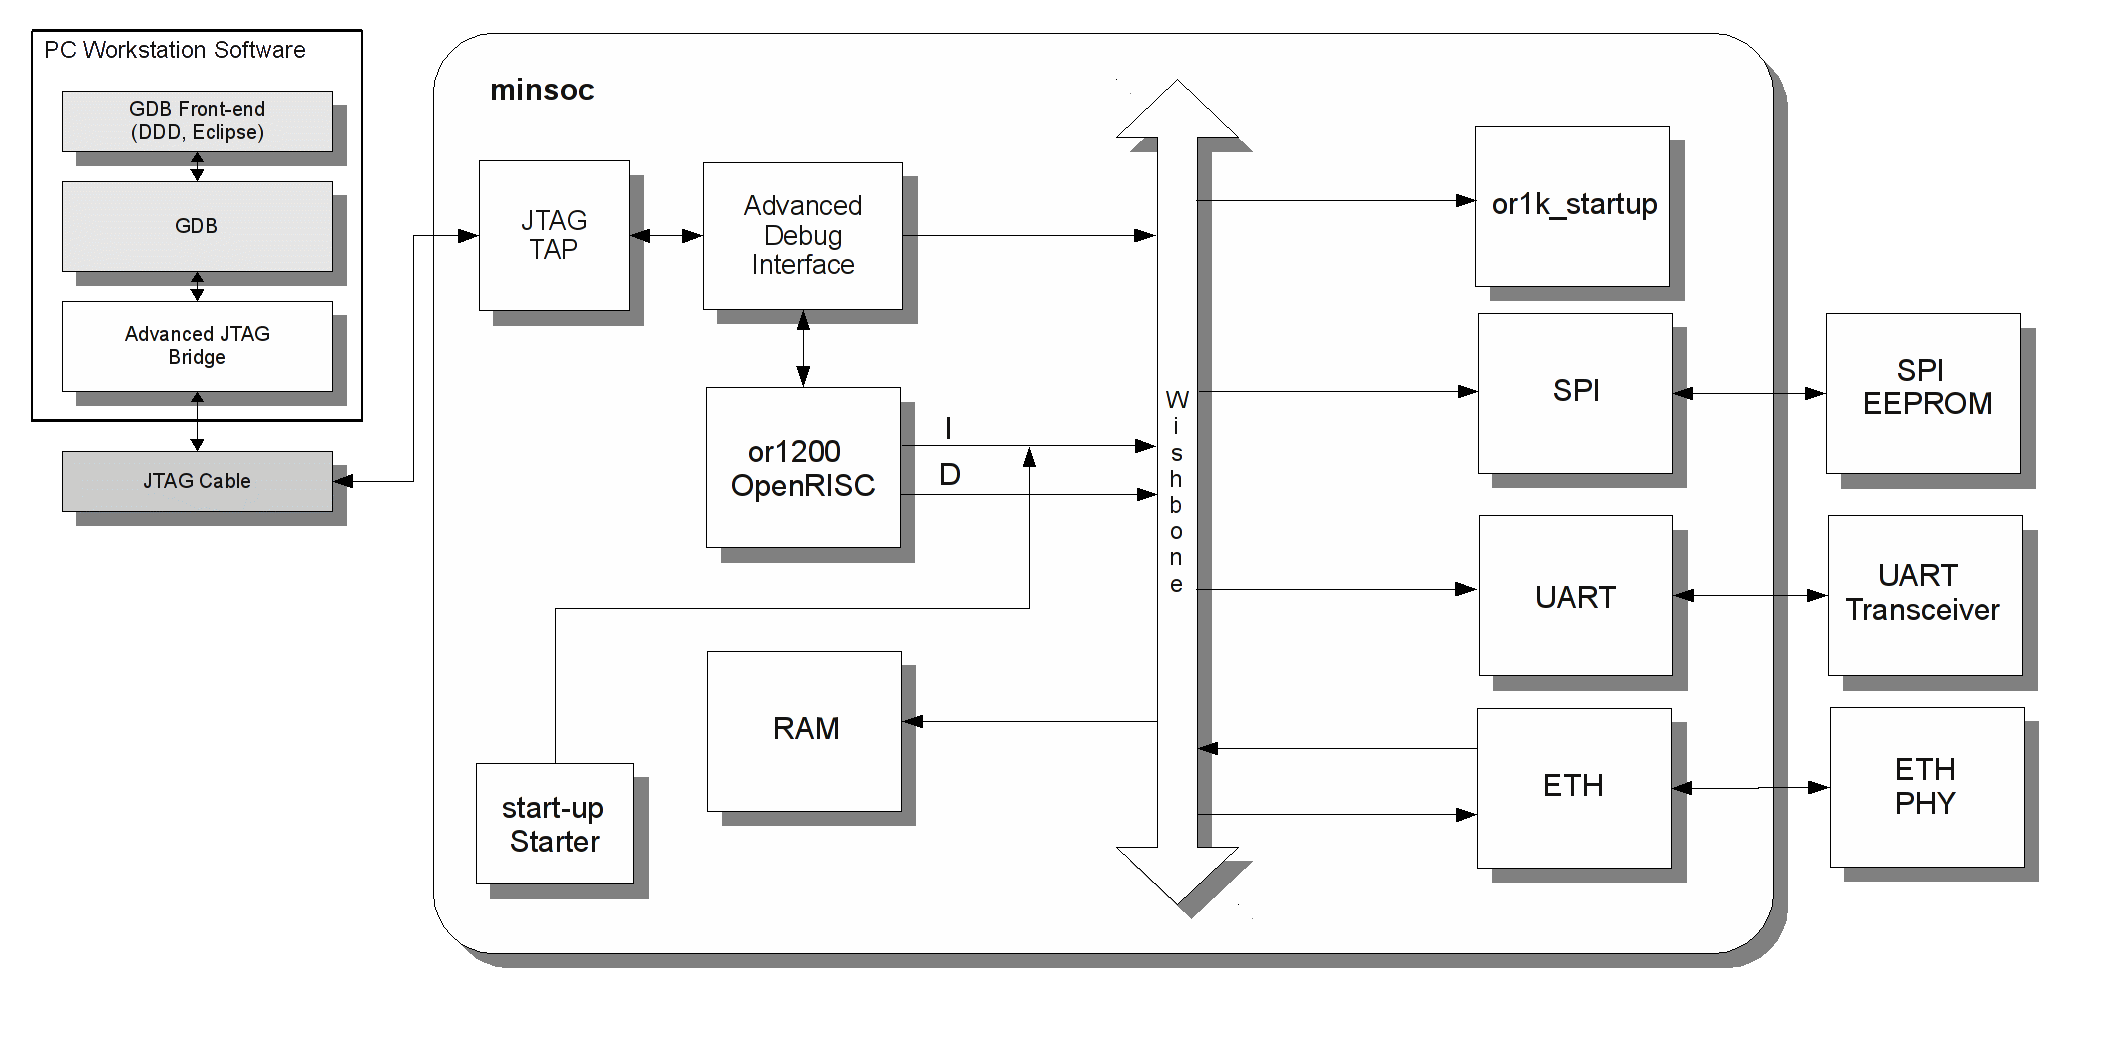
\includegraphics[width=1\textwidth,keepaspectratio=true]{./images/minsoc}
  \caption{Arquitectura MinSoc}
  \label{fig:esquema}
 \end{center}
\end{figure}

La guía práctica, está divida en dos partes principales: 

En la primera parte se detalla, principalmente, los pasos a seguir para poder configurar e implementar un SoC en la placa de desarrollo XILINX XtremeDSP Starter Platform Spartan 3A DSP 1800.


En la segunda parte se presenta la compilación cruzada con las herramientas de GNU para OpenRisc de un software de prueba, cargado a través del sistema de Debug Advanced con salida por modulo UART al puerto serie de la PC .

	%En la tercera parte se explica, además, lo problemas y soluciones para la implementación en el kit XILINX XtremeDSP Starter Platform Spartan 3A DSP 1800.

\newpage
\section{\textcolor{orange}{Objetivos del Proyecto MinSoc}}

La idea del proyecto es ofrecer un SoC sintetizable que sea  compatible con cualquier placa con una FPGA sin necesidad de modificaciones en su código RTL. El proyecto posee un depurador del sistema Debug Advanced,  el que permiten depurar el sistema con los mismos cables utilizados para la configuración de la FPGA. 

\section{\textcolor{orange}{Convenciones tipográficas}}

A largo de esta guía se utiliza la siguiente convención tipográfica: 

\begin{itemize}
\item Texto plano: se usa para indicar el contenido de un archivo, porciones de código y la salida que se muestra por consola al ingresar un comando.
\item Texto plano en negrita : se usa para indicar aquello que se ingresa por consola, usualmente, un comando. 
\item Texto plano entre corchetes angulares>: se usa para hacer referencia a un directorio. 
\item user@dist: se usa para indicar el prompt de la consola, tanto del host como del target. 
\end{itemize} 
 
Por ejemplo, la siguiente línea muestra que se ejecuta el comando ls en el directorio rootfs (que a  su vez se encuentra dentro del directorio\_ejemplo), en un host cuyo usuario es user y utiliza una distribuciòn dist de Linnux:


\begin{lstlisting}[breaklines]
user@dist:<directorio_ejemplo>/rootfs$ ls
\end{lstlisting}

\section{\textcolor{orange}{Requerimientos previos}}

 Para poder llevar a cabo la instalación de las herramientas de diseño de Hardware,sintetizar, implementar y efectuar debuging  del proyecto MinSoc en el kit de desarrollo, se necesita:

\begin{itemize}
\item Host de desarrollo con Ubuntu (12.4, preferentemente).
\item XILINX XtremeDSP Starter Platform Spartan 3A DSP 1800.
\item Xilinx ISE 14.2 con el directorio bin agregado al PATH.
\item Instalación del derive para el cable Platform Cable USB II.
\item Adaptador RS-232 a USB.
\item Emulador de consola.
\item Conexión a internet para descarga de paquetes.

\end{itemize} 

\newpage

\section{\textcolor{orange}{Dependencias}}

La instalación de las herramientas involucran la configuración previa de ciertas aplicaciones (como el tar) y la instalación de algunos paquetes.
Las siguientes son las dependencias necesarias para poder ejecutar el script de instalación del proyecto MinSoc

wget

svn

bzip2

tar

sed

patch

gcc

make

makeinfo

libncurses\-dev

flex

bison

libz\-dev 


 
\section{\textcolor{orange}{Instalación }}

El script de instalación funciona bajo cualquier Linux. Otros sistemas no son compatibles.

El script de instalación instala la cadena de herramientas GNU para OpenRISC, el adv\_ jtag\_ bridge para el software de carga y depuración y Icarus Verilog para la simulación del sistema. También descarga MinSoC y lo configura.
 

\subsection{\textcolor{orange}{Descarga de el script de instalación:}}

\begin{lstlisting}[breaklines]
 user@dist:~/$svn export http://opencores.org/ocsvn/minsoc/minsoc/tags/release-1.0/utils/
setup setup
\end{lstlisting}

\subsection{\textcolor{orange}{Ejecute el script de instalación}}

\begin{lstlisting}[breaklines]
user@dist:<directorio_de descarga_release-1.0>/minsoc/utils/setup$ minsoc-install.sh
\end{lstlisting}

La ejecución de este script requiere del usuario la ruta en la que se va a instalar el sistema.Por ejemplo:

\begin{lstlisting}[breaklines]
/home/user/Escritorio/minsoc
\end{lstlisting}

El sistema tiene la siguiente estructura de directorio después de ser ejecutado: 
\begin{lstlisting}[breaklines]
install_path/
	download/
	 tools/
 	 minsoc/
\end{lstlisting}

Todas las herramientas necesarias están instaladas en le directorio tools. Los paquetes descargados se encuentran en download y son compilados allí. El Advanced JTAG Bridge se agrega automáticamente a la ruta minsoc/rtl/verilog/adv\_debug\_sys/Software/adv\_jtag\_bridge  y también es compilado allí. 

Al final del script están incluidas las rutas de los binarios de las herramientas y los  binarios de el Toolchain de GNU en el directorio /home/user/.bashrc
 
Después de la correcta ejecución de el script, se pueden eliminar el directorio download y todo quedara instalado.

Antes de utilizar el sistema, se tiene que reiniciar el shell o cargar las nuevas variables de entorno ejecutando la linea de comando:

\begin{lstlisting}[breaklines]
user@dist:<directorio_de descarga_release-1.0>/minsoc/utils/setup$ sourece /home/user/.bashrc
\end{lstlisting}

\section{\textcolor{orange}{Síntesis}}

\subsection{\textcolor{orange}{Configuración de la placa especifica para la síntesis}}
Dentro del subdirectorio minsoc/backend/ se busca la placa en la que queremos implementar el proyecto MinSoc. Nos dirigimos al directorio correspondiente y ejecutamos el script de configuración.

\begin{lstlisting}[breaklines]
user@dist:<directorio_de_instalación>$cd minsoc/backend/spartan3a_dsp_kit 
user@dist:<directorio_de_instalación>/minsoc/backend/spartan3a_dsp_kit $./configure 
\end{lstlisting}

El sistema está configurado ahora, se puede proceder a la síntesis.

\subsection{\textcolor{orange}{Generación del .Bit}}

MinSoC utiliza un archivo Makefile para sintetizar su diseño. El sistema para sintetizar se encuentra en el subdirectorio minsoc/syn/xilinx. Una vez realizada la síntesis se creara el archivo .bit necesario para configurar la FPGA.

\begin{lstlisting}[breaklines]
user@dist:~<directorio_de_instalación>/minsoc/syn/xilinxt$make all
\end{lstlisting}

Después de que se ha generado el archivo de .bit, se cargar el archivo a la FPGA utilizando la herramienta del proveedor para este propósito como es en este caso iMPACT o mediante un herramienta Open Source llamada xc3sprog. 

\section{\textcolor{orange}{Complilacion de un Software para OpenRisc}}

Para compilar cualquier aplicación que vaya a ser ejecutada en el SoC con un micro OpenRisc, se necesita utilizar un compilador cruzado en este caso es el or32-elf-gcc que se encuentra incluido en el PATH por medio de el script de instalación minsoc-install.sh.

\begin{lstlisting}[breaklines]
user@dist:~<directorio_de_instalación>/minsoc/sw/uart$ make all
\end{lstlisting}
 
El comando make construye todas las librerías y archivos binarios, en este caso se creará el binario uart.or32 que sera cargado y debuging en el SoC.
 

Si tiene dudas sobre alguno de los comando/herramientas utilizados en esta sección se aconseja consultar al manual correspondiente a su terminal.


\section{\textcolor{orange}{Carga y Debugging de Software}}


Para conectar con éxito el TAP del SoC que contiene el micro OpenRISC , se debe copiar los archivos BSDL de todos los dispositivos conectados a la cadena de JTAG a un directorio conocido (por ejemplo /home/user/bsdl).Luego debe colocarse, el directorio como argumento al llamar adv\_jtag\_bridge, adv\_jtag\_bridge-b /home/user/bsdl.

\begin{enumerate}

\item Conecte el cable JTAG al TAP.
\item Inicio adv\_jtag\_bridge

\begin{lstlisting}[breaklines]
user@dist:~/$sudo adv_jtag_bridge -b<directorio_bsdl> xpc_usb 
\end{lstlisting}

Por ejemplo:

\begin{lstlisting}[breaklines]
user@dist:~/$sudo adv_jtag_bridge -b /home/user/bsdl xpc_usb 
\end{lstlisting}

El parametro -b <directorio\_bsdl> de adv\_jtag\_bridge para indicar el directorio donde obtener los archivos BSDL.

Al ser ejecutado en linux y utilizar cables xpc\_usb tiene que ejecutarse como superusuario.


\item Una vez que el programa se encuentre en funcionamiento se debe abrir otro terminal (por ejemplo gtkterm).
\item Configuramos el puerto a un puerto serie conectado a la placa.
\item Configuramos el bitrete a 115200.

\item Se inicia gdb y se carga el firmware de ejemplo compilado previamente para OpenRisc.

\item 
\begin{lstlisting}[breaklines]
user@dist:~/<directorio_de_instalación>minsoc/sw/uart$ or32-elf-gdb uart.or32
target remote :9999
load
set $pc=0x100
c
\end{lstlisting}

\item Dentro de gtkterm debería haber aparecido "Hello World". 

\end{enumerate}

%\newpage
%\section{\textcolor{orange}{Problemas y soluciones}}

\newpage

\section{\textcolor{orange}{Acrónimos y abreviaturas}}

\begin{table}[!h]
\begin{center}
\begin{tabular}{|c|c|}
\hline
\rowcolor[RGB]{255,127,0} Abreviatura & Significado en ingles \\
\hline
FPGA & Field Programmable Gate Array  \\
\hline
TAP & Test Access Port  \\
\hline
\hline
BSDL & Boundary Scan Description Language  \\
\hline
\hline
JTAG & Joint Test Action Group  \\
\hline
\hline
SoC & System on Chip\\
\hline
\hline
RAM & Andom Access Memory \\
\hline
\hline
USB & Universal Serial Bus  \\
\hline
\hline
DSP& Digital Signal Processing \\
\hline
\hline
RTL & Register transfer level \\
\hline
\hline
GNU & GNU is not Unix\\
\hline
\end{tabular}
\end{center}
\end{table}

\newpage

\section{\textcolor{orange}{Bibliografía}}
\subsection{\textcolor{orange}{Documentos}}
\begin{itemize}
\item Spartan\-3A DSP Starter Platform User Guide\url{http://www.xilinx.com/support/documentation/boards_and_kits/ug454_sp3a_dsp_start_ug.pdf}.
\item Matthew Hicks. University of Illinois at Urbana\-Champaign. "guideTop".  
\end{itemize} 
\subsection{\textcolor{orange}{sitios web}}
\begin{itemize}
\item \url{http://www.minsoc.com/}
\item \url{http://opencores.org/or1k/OR1200_OpenRISC_Processor}
\item\url{http://www.xilinx.com/products/boards-and-kits/HW-SD1800A-DSP-SB-UNI-G.htm}

\end{itemize} 



 \newpage
 \chapter{Guía Básica de Implementación para ORPSoC}

 \section{Introdución}
Este proyecto implementa una plataforma para el desarrollo OpenRISC. Proporciona un SoC de referencia, para la prueba y el desarrollo de procesadores OpenRISC.

 \section{Descarga del ORPSoC}
La el código fuente RTL, el software de prueba y scripts de instalación pueden ser descargados del repositorio svn del proyecto OpenRISC. Los archivos pueden descargados con el siguiente comandos.

\begin{lstlisting}[breaklines]
 usuario@usuario-desktop:~/$  svn co http://opencores.org/ocsvn/openrisc/openrisc/trunk/orpsocv2
\end{lstlisting}

Después de descomprimir el archivo descargado para la instalación ORPSoC se parece a esto ~\ref{fig:esquema} 

\begin{figure}[h!]
 \begin{center}
  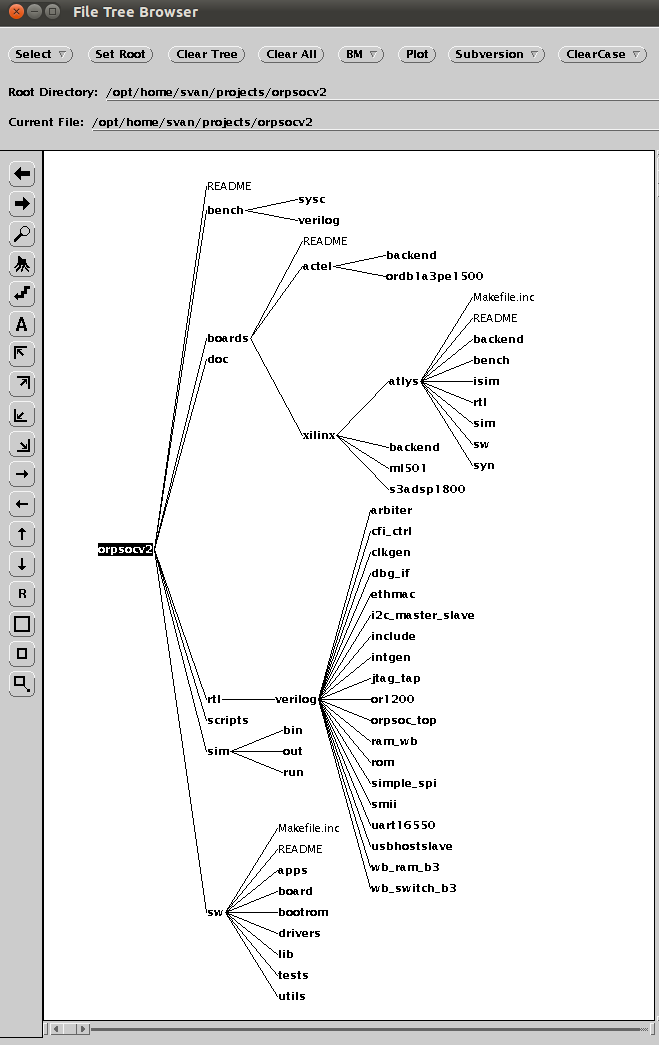
\includegraphics[width=0.8\textwidth,keepaspectratio=true]{./images/proyectoorpsoc}
  \caption{Esquema del Proyecto ORPSoC }
  \label{fig:esquema}
 \end{center}
\end{figure}

 \section{Instalación de herramientas}
 \subsection{Instalación de herramientas GNU}

Los programas deben ser instalados en el directorio / opt. Utilice los siguientes comandos para descomprimir y descomprimir el archivo descargado: 


 \section{Instalación de herramientas Xilinx}

Antes de realizar esto necesitamos tener instaladas correctamente las herramientas de Xilinix. Luego de la instalación debemos agregar al PATH de Linux las rutas a los binarios necesarios para realizar el proceso. 

\begin{lstlisting}[breaklines]
 usuario@usuario-desktop:~/$ source (ruta a Xilinx ISE)/settings32.sh  
\end{lstlisting}

 \section{Syntesis}
La construcción del proyecto está configurada para el uso de Makefiles. Los pasos a realizar son los siguientes:

\begin{itemize}
\item Los archivos necesarios para realizar la síntesis se encuentran en 

\begin{lstlisting}[breaklines]
(orpsoc_dir)/boards/xilinx/(board)/syn/
\end{lstlisting}

\item Limpiamos cualquier síntesis anteriormente realizada 
\begin{lstlisting}[breaklines]
usuario@usuario-desktop:(orpsoc_dir)/boards/xilinx/s3adsp1800/syn/xst/run$ make clean
\end{lstlisting}

\item Verificamos que solo existe el makefile
\begin{lstlisting}[breaklines]
usuario@usuario-desktop:(orpsoc_dir)/boards/xilinx/s3adsp1800/syn/xst/run$ ls

Makefile
\end{lstlisting}

\item Realizamos una nueva síntesis
\begin{lstlisting}[breaklines]
usuario@usuario-desktop:(orpsoc_dir)/boards/xilinx/s3adsp1800/syn/xst/run$ make all
\end{lstlisting}

\end{itemize} 

% #### Generating Xilinx PRJ file ####
% #### Generating XST file ####
% #### Generating Xilinx XCF file ####
% #### Running XST ####

\section{Place and Route}
%///////////// Place and Route ////////////////////////
Luego de la síntesis para realizar el procedimiento Place and Route (PAR) debemos ir a la carpeta
\begin{lstlisting}[breaklines]
(orpsoc_dir)/boards/xilinx/(board)/backend/par/
\end{lstlisting}
Limpiamos cualquier PAR anteriormente realizado

\begin{lstlisting}[breaklines]
usuario@usuario-desktop:(orpsoc_dir)/boards/xilinx/s3adsp1800/backend/par/run$ make clean
\end{lstlisting}

Verificamos que solo existe el makefile
\begin{lstlisting}[breaklines]
usuario@usuario-desktop:(orpsoc_dir)/boards/xilinx/s3adsp1800/backend/par/run$ ls
Makefile
\end{lstlisting}

Realizamos el proceso PAR 

\begin{lstlisting}[breaklines]
usuario@usuario-desktop:(orpsoc_dir)/boards/xilinx/s3adsp1800/backend/par/run$ make orpsoc.ncd
\end{lstlisting}
El reporte del PAR se encuentra en 
\begin{lstlisting}[breaklines]
usuario@usuario-desktop:(orpsoc_dir)/boards/xilinx/s3adsp1800/backend/par/run$ cat orpsoc.par
\end{lstlisting}

Para listar los valores de configuración con las que se esta realizando el proceso
\begin{lstlisting}[breaklines]
usuario@usuario-desktop:(orpsoc_dir)/boards/xilinx/s3adsp1800/backend/par/run$ make print-config
\end{lstlisting}

Para realizar un informe de "timing post place" 

\begin{lstlisting}[breaklines]
usuario@usuario-desktop:(orpsoc_dir)/boards/xilinx/s3adsp1800/backend/par/run$ make timingreport
\end{lstlisting}

El informe se encuentra en:

\begin{lstlisting}[breaklines]
usuario@usuario-desktop:(orpsoc_dir)/boards/xilinx/s3adsp1800/backend/par/run$ cat orpsoc.twr | less
\end{lstlisting}


 \section{Generación del .Bit}

Finalmente generamos el bitfile que contiene la configuración que debemos cargar en la FPGA.

\begin{lstlisting}[breaklines]
usuario@usuario-desktop:(orpsoc_dir)/boards/xilinx/s3adsp1800/backend/par/run$ make orpsoc.bit
\end{lstlisting}

 \section{Configuración de la FPGA}

%//////////// XC3SPROG INSTALLATION   //////////////
Para descargar el bitfile de configuración utilizamos xc3sprog y un programador basado en FTDI2232. Este hardware requiere de la herramienta 

Descargamos el código del programa
\begin{lstlisting}[breaklines]
usuario@usuario-desktop:~/$ svn checkout svn://svn.code.sf.net/p/xc3sprog/code/trunk xc3sprog-code
usuario@usuario-desktop:~/$ cd xc3sprog-code
usuario@usuario-desktop:~/$   
\end{lstlisting}
%........   TERMINAR PROCESO DE COMPILACIÓN ..... 


%//////////// DOWNLOAD THE BITSTREAM ON FPGA   //////////////

Luego de conectar el programador en el conector J4. Chequeamos el funcionamiento escaneando la cadena JTAG
\begin{lstlisting}[breaklines]
usuario@usuario-desktop:~$ sudo (ruta a xc3sprog)/xc3sprog  -c ftdi -j
usuario@usuario-desktop:(orpsoc_dir)/boards/xilinx/s3adsp1800/backend/par/run$ sudo (ruta a xc3sprog)/xc3sprog  -c ftdi  orpsoc.bit 
\end{lstlisting}

 \section{Descarga del BITSTREAM a la SPI }

%//////////// DOWNLOAD THE BITSTREAM ON SPI   //////////////
Inicialmente descargamos el bitfile provisto en la carperta
\begin{lstlisting}[breaklines]
xc3sprog/bscan_files
\end{lstlisting} 
 que configura la fpga para actuar como intermediario ante la FLASH SPI y así lograr grabar en la misma.
\begin{lstlisting}[breaklines]
usuario@usuario-desktop:(orpsoc_dir)/boards/xilinx/s3adsp1800/backend/par/run$ sudo (ruta a xc3sprog)/xc3sprog  -c ftdi (ruta a xc3sprog)/bscan_spi/xc3sd1800-fg676.bit 
\end{lstlisting} 

Ahora podemos descargar el bitstream a la FLASH SPI mediante 
\begin{lstlisting}[breaklines]
usuario@usuario-desktop:(orpsoc_dir)/boards/xilinx/s3adsp1800/backend/par/run$ sudo (ruta a xc3sprog)/xc3sprog  -c ftdi  -I orpsoc.bit 
\end{lstlisting}
 \newpage
 
\chapter{Códigos de Prueba}

 \section{Introducción}

En el presente anexo se  publicaran los corresppndientes códigos que se realizaron con el fin de probar el correcto funcionamiento de los requerimientos e los diferentes prototipos


 \section{Programa de Prueba para el UART}

\begin{lstlisting}[language=C,frame=single]
#include <board.h>
#include <support.h>
#include <or1200.h>
#include <int.h>

#include <uart.h>

int main()
{
	uart_init();
	int_init();
	int_add(UART_IRQ, &uart_interrupt, NULL);
	
	/* We can't use printf because in this simple example
	   we don't link C library. */
	uart_print_str("Hello World.\n");
	
	report(0xdeaddead);
	or32_exit(0);
}

\end{lstlisting}

 \section{Programa de Prueba para Ethernet}

\begin{lstlisting}[language=C,frame=single]
#include <board.h>
#include <support.h>
#include <or1200.h>
#include <int.h>

#include <uart.h>
#include <eth.h>


extern int eth_rx_len;
extern int eth_rx_done, eth_tx_done;
extern unsigned char * eth_rx_data;
extern unsigned char * eth_tx_data;

void eth_receive()
{
	int i;
	uart_print_str("Length: \n");
	uart_print_long(eth_rx_len);
	uart_print_str("\n");
	uart_print_str("Data: \n");
	for ( i = 0; i < eth_rx_len; i++ )
	{
		uart_print_short(eth_rx_data[i]);
		uart_print_str("\n");
	}
	eth_recv_ack();
}

int main()
{
	uart_init();

	int_init();
	eth_init();
	int_add(UART_IRQ, &uart_interrupt, NULL);
	int_add(ETH_IRQ, &eth_interrupt, NULL);

	/* We can't use printf because in this simple example
	   we don't link C library. */
	uart_print_str("Hello World.\n");

	eth_tx_data[0] = 0xFF;
	eth_tx_data[1] = 0x2B;
	eth_tx_data[2] = 0x40;
	eth_tx_data[3] = 0x50;

	eth_send(4);

	while(1)
	{
		if (eth_rx_done)
		{
			eth_receive();
		}
	}

	report(0xdeaddead);
	or32_exit(0);
}
\end{lstlisting}


 \section{Programa de Prueba para Capacidad de Procesamiento}

\begin{lstlisting}[language=C,frame=single]
#include <board.h>
#include <support.h>
#include <or1200.h>
#include <int.h>
#include <uart.h>

#define con 15
#define N 16

void genmatriz(unsigned seed1,unsigned *matriz,int indice){
/*
    uart_print_str("seed ="); 
    uart_print_long(seed1);
    uart_print_str("\n");
*/    
    unsigned sr1[N] ;
    unsigned i , j ,q  ;
    unsigned tmp;    
    
    for(i=0; i<N; i++){
  	sr1[i] =  (seed1&1);
  	seed1/=2;
    }

    for (q=0;q<(indice*indice);q++){
		tmp = sr1[15]^sr1[14]^sr1[13]^sr1[11];
		
		for(j=N;j>0;j--) sr1[j]=sr1[j-1];
		sr1[0] = tmp;

		matriz[q] = tmp;
		
                //uart_print_long(tmp);
		//if (((q+1)%con_i)==0) uart_print_str("\n");
    }   

}


int main()
{
 
    // Declaraciones
    int i , j , k ; 
    int indice;
    unsigned matriz  [con*con];
    unsigned matrizA [con*con];
    unsigned matrizB [con*con];
    
    int producto ; 
    int acumulador ;
    unsigned tiempo;
    int useg;

	

////// Setup Inicial
    //tick_init();
    asm("l.mtspr\t\t%0,%1,0": : "r" (SPR_TTMR), "r" (SPR_TTMR_CR));
    asm("l.mtspr\t\t%0,%1,0": : "r" (SPR_TTCR), "r" (0x0));
    //mtspr(SPR_TTCR, SPR_TTMR_CR);
    //mtspr(SPR_TTCR, 0x0);
        
    //tick_start();
    asm("l.mtspr\t\t%0,%1,0": : "r" (SPR_TTCR), "r" (0x0));
    //mtspr(SPR_TTCR, 0x0);
    
    tiempo = mfspr(SPR_TTCR);
    useg = (int) tiempo * 50 ;
    uart_print_str("Tick de ejecucion setup tick :");
    uart_print_long((long)tiempo);
    uart_print_str(" En us = ");
    uart_print_long(useg);
    uart_print_str("\n");   
   
    for (indice=1; indice<=con; indice++){
    //tick_start();
    //asm("l.mtspr\t\t%0,%1,0": : "r" (SPR_TTCR), "r" (0x0));
    //uart_print_str("Matrices de  :");
    uart_print_long(indice);
    uart_print_str(",");
    //uart_print_str("\n");

 
    mtspr(SPR_TTCR, 0x0);
    
    i= 0;
    j= 0;
    k= 0;
    producto = 0;
    acumulador = 0;
/*
    for (i=0;i<indice;i++){
		for (j=0;j<indice;j++){
			matriz  [i][j] = 0;
			matrizA [i][j] = 1;
			matrizB [i][j] = 1;
		}
	}
*/
      tiempo = mfspr(SPR_TTCR);
      genmatriz (tiempo,matriz,indice);
      tiempo = mfspr(SPR_TTCR);
      genmatriz (tiempo,matrizA,indice);
      tiempo = mfspr(SPR_TTCR);
      genmatriz (tiempo,matrizB,indice);
    

//    tiempo = mfspr(SPR_TTCR);
//    useg = (int) tiempo * 50 ; 
//    uart_print_str("Tick de ejecucion seteo de variables :");
//    uart_print_long((long)tiempo);
//    uart_print_str(" En us = ");
//    uart_print_long(useg);
// 	uart_print_str("\n");
 	 
 
	mtspr(SPR_TTCR, 0x0);
    
	for (i=0;i<indice;i++){
		for (j=0;j<indice;j++){
			for (k=0;k<indice;k++){
				producto = matrizA[i*con+k] * matrizB[k*con+j];
				acumulador = acumulador + producto;
			}
			matriz [i*con+j] = acumulador;
			acumulador = 0;
		}	
	}
    
    tiempo = mfspr(SPR_TTCR);
//    useg = (int) tiempo * 50 ;
//    uart_print_str("Tick de ejecucion de la multiplicacion :");
    uart_print_long((long)tiempo);
//    uart_print_str(" En us = ");
//    uart_print_long(useg);
    uart_print_str("\n");   
    

/*
    uart_print_str("Matriz Resultado");   
    uart_print_str("\n");   
    
    for (i=0;i<indice;i++){
		for (j=0;j<indice;j++){
			uart_print_long(matriz [i*con+j]);
			uart_print_str(" ");
		}
		uart_print_str("\n");
	}
  
 */  
    } 
  
    uart_print_str("Fin del programa\n");

    return 0;
}
\end{lstlisting}

 \subsection{Generador de secuencia binaria seuda aleatoria}
\begin{lstlisting}[language=C,frame=single]
#include "stdio.h"
#include "time.h"
#define con_i 10

#define N 16

void genmatriz(unsigned seed1,unsigned *matriz){
    printf ("seed1 ="); 
    printf("%x",seed1);
    printf("\n");   
    
    //unsigned  seed1 ; 
    unsigned sr1[N] ;
    unsigned i , j ,q  ;
    unsigned tmp;    
    
    for(i=0; i<N; i++){
  	sr1[i] =  (seed1&1);
  	seed1/=2;
    }

    for (q=0;q<(con_i*con_i);q++){
		tmp = sr1[15]^sr1[14]^sr1[13]^sr1[11];
		
		for(j=N;j>0;j--) sr1[j]=sr1[j-1];
		sr1[0] = tmp;

		matriz[q] = tmp;
		
                //printf ("%i ",tmp);
		//if (((q+1)%con_i)==0) printf ("\n");
    }   
	printf ("\n\n");
}

int main(void ) {

unsigned matriz[100] ;
unsigned i,j ;
genmatriz (time(NULL),matriz);
for (i=0;i<100;i++){
	printf ("%i ",matriz[i]);
	if (((i+1)%10)==0) printf ("\n");
}

 return 0;
}
\end{lstlisting}

 \section{Programa de Prueba de SDRAM}
 \begin{lstlisting}[language=C,frame=single]
 #include "cpu-utils.h"
#include "board.h"
#include "sdram.h"
#include "uart.h"
#include "printf.h"

#ifndef _SDRAM_H_
#define _SDRAM_H_

#ifdef  MT48LC32M16A2 // 64MB SDRAM part
#define SDRAM_SIZE 0x04000000
#define SDRAM_ROW_SIZE 2048 // in bytes (10 bits col addr, 2 bytes per)
#define SDRAM_NUM_ROWS_PER_BANK (8192) // 13-bit row address
#define SDRAM_NUM_BANKS 4
#endif

#ifdef  MT48LC16M16A2 // 32MB SDRAM part
#define SDRAM_SIZE 0x02000000
#define SDRAM_ROW_SIZE 1024 // in bytes (9 bits col addr, 2 bytes per)
#define SDRAM_NUM_ROWS_PER_BANK (8192) // 13-bit row address
#define SDRAM_NUM_BANKS 4
#endif

#ifdef MT48LC4M16A2 // 8MB SDRAM part
#define SDRAM_SIZE 0x800000
#define SDRAM_ROW_SIZE 512 // in bytes (8 bits col addr, 2 bytes per)
#define SDRAM_NUM_ROWS_PER_BANK (4096) // 12-bit row address
#define SDRAM_NUM_BANKS 4
#endif


#endif


#define SDRAM_NUM_ROWS (SDRAM_NUM_ROWS_PER_BANK * SDRAM_NUM_BANKS)

#define START_ROW 128

int main()
{

  uart_init(DEFAULT_UART);


  printf("\n\tSDRAM rows test\n");

  printf("\n\tWriting\n");
  
  int i; // Skip first 64KB, code/stack resides there - TODO determine this from
  // stack linker variable!
  for(i=START_ROW;i<(SDRAM_NUM_ROWS);i++)
    {
      REG32((i*(SDRAM_ROW_SIZE))) = i;
      printf("\r\t0x%x", i);
    }

  printf("\n\tReading\n");

  int read_result = 0;

  for(i=START_ROW;i<(SDRAM_NUM_ROWS);i++)
    {
      printf("\r\t0x%x", i);
      read_result = REG32((i*(SDRAM_ROW_SIZE)));
      if (read_result != i)
	{
	  printf("\n\Error at 0x%x, read 0x%x, expected 0x%x\n",
		 (i*SDRAM_ROW_SIZE), read_result, i);
	  report(0xbaaaaaad);
	  report(i);
	  report(read_result);
	  exit(0xbaaaaaad);
	}
    }
  printf("\n\tTest OK.\n");
  exit(0x8000000d);  
}
 
 \end{lstlisting}

 \section{Programa de Prueba Ethernet del Proyecto ORPSoC}
 \begin{lstlisting}[language=C,frame=single]
 
int main ()
{
  
	print_packet_contents = 0; // Default to not printing packet contents.
	packet_inspect_debug = 0;
	print_ethmac_debug_reg = 0;

	/* Initialise vector handler */
	int_init();

	/* Install ethernet interrupt handler, it is enabled here too */
	int_add(ETH0_IRQ, oeth_interrupt, 0);

	/* Enable interrupts */
	cpu_enable_user_interrupts();
    
	last_char=0; /* Variable init for spin_cursor() */
	next_tx_buf_num = 4; /* init for tx buffer counter */

	uart_init(DEFAULT_UART); // init the UART before we can printf
	printf("\n\teth ping program\n\n");
	printf("\n\tboard IP: %d.%d.%d.%d\n",our_ip[0]&0xff,our_ip[1]&0xff,
	       our_ip[2]&0xff,our_ip[3]&0xff);
  
	ethmac_setup(); /* Configure MAC, TX/RX BDs and enable RX and TX in 
			   MODER */
  
	//scan_ethphys(); /* Scan MIIM bus for PHYs */
	//ethphy_init(); /* Attempt reset and configuration of PHY via MIIM */
	//ethmac_scanstatus(); /* Enable scanning of status register via MIIM */

	/* Loop, monitoring user input from TTY */
	while(1)  
	{
		char c;
      
		while(!uart_check_for_char(DEFAULT_UART))
		{
			
			spin_cursor();
			
			if (print_ethmac_debug_reg)
				oeth_print_wbdebug();
		}
      
		c = uart_getc(DEFAULT_UART);

		if (c == 's')
			tx_packet((void*) ping_packet, 98);
		else if (c == 'S')
			tx_packet((void*)big_ping_packet, 1514);
		else if (c == 'h')
			scan_ethphys();
		else if (c == 'i')
			ethphy_init();
		else if (c == 'c')
			oeth_ctrlmode_switch();
		else if (c == 'P')
		{
			print_packet_contents = print_packet_contents ? 0 : 1;
			if (print_packet_contents)
				printf("Enabling packet dumping\n");
			else
				printf("Packet dumping disabled\n");
		}
		else if (c == 'p')
			oeth_printregs();
		else if (c == 'a')
			ethphy_print_status(ethphy_found);
		else if (c >= '0' && c <= '9')
			scan_ethphy(c - 0x30);
		else if (c == 'r')
		{
			ethphy_reset(ethphy_found);
			printf("PHY reset\n");
		}
		else if (c == 'R')
		{
			//oeth_reset_tx_bd_pointer();
			ethmac_setup();
			printf("MAC reset\n");
		}
		else if (c == 'n')
			ethphy_reneg(ethphy_found);
		else if (c == 'N')
			ethphy_toggle_autoneg(ethphy_found);
		else if (c == 'm')
			ethmac_togglehugen();
		else if (c == 't')
			ethphy_set_10mbit(ethphy_found);
		else if (c == 'H')
			ethphy_set_100mbit(ethphy_found);
		else if ( c == 'b' )
		{
			printf("\n\t---\n");
			oeth_dump_bds();
			printf("\t---\n");
		}
      
		else if ( c == 'B' )
		{
			tx_packet((void*) broadcast_ping_packet, 298);
		}
		else if (c == 'u' )
			oeth_transmit_pause();
		else if (c == 'd' )
		{
			oeth_print_wbdebug();
			print_ethmac_debug_reg = !print_ethmac_debug_reg;
		}
		else if (c == 'D')
		{
			marvell_phy_toggle_delay();
		}
		else if (c == 'v' )
		{
			if (packet_inspect_debug)
				printf("Disabling ");
			else 
				printf("Enabling ");
			
			printf("packet type announcments\n");
			
			packet_inspect_debug = !packet_inspect_debug;
		}
		else if ( c == 'o' )
			oeth_toggle_promiscuous();
		else if (c == 'L')
			ethphy_toggle_loopback();
		else if (c == 'g')
			ethphy_toggle_gigadvertise();

	}
	 \end{lstlisting}
	 
	  \section{Programa de Prueba de Compilador y Depurador para ORPSoC - Números Primos}
 \begin{lstlisting}[language=C,frame=single]
Código de prueba de numeros primos 
	 \end{lstlisting}
	
 \newpage

 %\chapter{MANUAL DE USUARIO: INTERFAZ GRAFICA}
 %\input{manual_gui}          
\newpage
\end{part}

\end{document}
